%\VignetteIndexEntry{Introduction to the EGRET package}
%\VignetteEngine{knitr::knitr}
%\VignetteDepends{}
%\VignetteSuggests{xtable, dataRetrieval}
%\VignetteImports{methods,survival, fields}
%\VignettePackage{EGRET}

\documentclass[a4paper,11pt]{article}\usepackage{graphicx, color}
%% maxwidth is the original width if it is less than linewidth
%% otherwise use linewidth (to make sure the graphics do not exceed the margin)
\makeatletter
\def\maxwidth{ %
  \ifdim\Gin@nat@width>\linewidth
    \linewidth
  \else
    \Gin@nat@width
  \fi
}
\makeatother

\definecolor{fgcolor}{rgb}{0.2, 0.2, 0.2}
\newcommand{\hlnumber}[1]{\textcolor[rgb]{0,0,0}{#1}}%
\newcommand{\hlfunctioncall}[1]{\textcolor[rgb]{0.501960784313725,0,0.329411764705882}{\textbf{#1}}}%
\newcommand{\hlstring}[1]{\textcolor[rgb]{0.6,0.6,1}{#1}}%
\newcommand{\hlkeyword}[1]{\textcolor[rgb]{0,0,0}{\textbf{#1}}}%
\newcommand{\hlargument}[1]{\textcolor[rgb]{0.690196078431373,0.250980392156863,0.0196078431372549}{#1}}%
\newcommand{\hlcomment}[1]{\textcolor[rgb]{0.180392156862745,0.6,0.341176470588235}{#1}}%
\newcommand{\hlroxygencomment}[1]{\textcolor[rgb]{0.43921568627451,0.47843137254902,0.701960784313725}{#1}}%
\newcommand{\hlformalargs}[1]{\textcolor[rgb]{0.690196078431373,0.250980392156863,0.0196078431372549}{#1}}%
\newcommand{\hleqformalargs}[1]{\textcolor[rgb]{0.690196078431373,0.250980392156863,0.0196078431372549}{#1}}%
\newcommand{\hlassignement}[1]{\textcolor[rgb]{0,0,0}{\textbf{#1}}}%
\newcommand{\hlpackage}[1]{\textcolor[rgb]{0.588235294117647,0.709803921568627,0.145098039215686}{#1}}%
\newcommand{\hlslot}[1]{\textit{#1}}%
\newcommand{\hlsymbol}[1]{\textcolor[rgb]{0,0,0}{#1}}%
\newcommand{\hlprompt}[1]{\textcolor[rgb]{0.2,0.2,0.2}{#1}}%

\usepackage{framed}
\makeatletter
\newenvironment{kframe}{%
 \def\at@end@of@kframe{}%
 \ifinner\ifhmode%
  \def\at@end@of@kframe{\end{minipage}}%
  \begin{minipage}{\columnwidth}%
 \fi\fi%
 \def\FrameCommand##1{\hskip\@totalleftmargin \hskip-\fboxsep
 \colorbox{shadecolor}{##1}\hskip-\fboxsep
     % There is no \\@totalrightmargin, so:
     \hskip-\linewidth \hskip-\@totalleftmargin \hskip\columnwidth}%
 \MakeFramed {\advance\hsize-\width
   \@totalleftmargin\z@ \linewidth\hsize
   \@setminipage}}%
 {\par\unskip\endMakeFramed%
 \at@end@of@kframe}
\makeatother

\definecolor{shadecolor}{rgb}{.97, .97, .97}
\definecolor{messagecolor}{rgb}{0, 0, 0}
\definecolor{warningcolor}{rgb}{1, 0, 1}
\definecolor{errorcolor}{rgb}{1, 0, 0}
\newenvironment{knitrout}{}{} % an empty environment to be redefined in TeX

\usepackage{alltt}

\usepackage{amsmath}
\usepackage{times}
\usepackage{hyperref}
\usepackage[numbers, round]{natbib}
\usepackage[american]{babel}
\usepackage{authblk}
\usepackage{subfig}
\usepackage{placeins}
\usepackage{footnote}
\usepackage{tabularx}
\renewcommand\Affilfont{\itshape\small}

\renewcommand{\topfraction}{0.85}
\renewcommand{\textfraction}{0.1}
\usepackage{graphicx}

\textwidth=6.2in
\textheight=8.5in
\parskip=.3cm
\oddsidemargin=.1in
\evensidemargin=.1in
\headheight=-.3in

%------------------------------------------------------------
% newcommand
%------------------------------------------------------------
\newcommand{\scscst}{\scriptscriptstyle}
\newcommand{\scst}{\scriptstyle}
\newcommand{\Robject}[1]{{\texttt{#1}}}
\newcommand{\Rfunction}[1]{{\texttt{#1}}}
\newcommand{\Rclass}[1]{\textit{#1}}
\newcommand{\Rpackage}[1]{\textit{#1}}
\newcommand{\Rexpression}[1]{\texttt{#1}}
\newcommand{\Rmethod}[1]{{\texttt{#1}}}
\newcommand{\Rfunarg}[1]{{\texttt{#1}}}
\IfFileExists{upquote.sty}{\usepackage{upquote}}{}

\begin{document}








%------------------------------------------------------------
\title{Introduction to the EGRET package}
%------------------------------------------------------------
\author[1]{Robert Hirsch}
\author[1]{Laura De Cicco}
\affil[1]{United States Geological Survey}

\maketitle

Exploration and Graphics for RivEr Trends (EGRET): An R-package for the analysis of long-term changes in water quality and streamflow, including the water-quality method Weighted Regressions on Time, Discharge, and Season (WRTDS)

\tableofcontents

%------------------------------------------------------------
\section{Introduction to Exploration and Graphics for RivEr Trends (EGRET)}
%------------------------------------------------------------ 

Exploration and Graphics for RivEr Trends (EGRET): An R-package for the analysis of long-term changes in water quality and streamflow. EGRET includes statistics and graphics for streamflow history, water quality trends, and the modeling algorithm Weighted Regressions on Time, Discharge, and Season (WRTDS). 


\textbf{Please see the official EGRET manual:}
(\href{https://github.com/USGS-R/EGRET/raw/Documentation/EGRET%2Bmanual_4.doc}{link to download}) 
\textbf{for more information on the EGRET package.}

For information on getting started in R, downloading and installing the package, see Appendix 1:

The best way to learn about the WRTDS approach and to see examples of its application to multiple large data sets is to read two journal articles.  They are available, for free, from the journals in which they were published.

The first relates to nitrate and total phosphorus data for 9 rivers draining to Chesapeake Bay.  The URL is \cite{HirschII}: 
\url{http://onlinelibrary.wiley.com/doi/10.1111/j.1752-1688.2010.00482.x/full}

The second is an application  to nitrate data for 8 monitoring sites on the Mississippi River or its major tributaries \cite{HirschIII}.  The URL is: \url{http://pubs.acs.org/doi/abs/10.1021/es201221s}

This vignette assumes that the user understands the concepts underlying WRTDS.  Thus, reading at least the first of these papers is necessary for understanding.  The method has been enhanced beyond what was published there.  The enhancement is that it now properly handles censored data by using survival regression rather than ordinary regression.  The details of that are in a report on Chesapeake Bay river input trends \cite{HirschIV}:\url{http://pubs.usgs.gov/sir/2012/5244/}.  The specific enhancements for handling censored data are on pages 9-11 of that report.

This vignette will walk through the major functions provided by the EGRET package. The package dataRetrieval is required for importing data in an EGRET-friendly format. The dataRetrieval package, along with installation instructions can be found at:
\url{https://github.com/USGS-R/dataRetrieval}

Installing dataRetrieval will provide a vignette similar to this document, with complete working examples of the main dataRetrieval functions.

This document assumes the reader is familiar with the dataRetrieval package. Further details can be found in the user guide that can be found on gitHub: \url{https://github.com/USGS-R/EGRET/raw/Documentation/EGRET%2Bmanual_4.doc}

%------------------------------------------------------------
\section{EGRET Workflow}
%------------------------------------------------------------ 
Subsequent sections of this vignette will discuss the EGRET workflow steps in greater detail. This section provides a handy cheat sheet for diving into an EGRET analysis.

\begin{knitrout}
\definecolor{shadecolor}{rgb}{0.969, 0.969, 0.969}\color{fgcolor}\begin{kframe}
\begin{alltt}
\hlfunctioncall{library}(dataRetrieval)
\hlfunctioncall{library}(EGRET)

\hlcomment{############################}
\hlcomment{# Gather discharge data:}
siteID <- \hlstring{"01491000"} #Choptank River at Greensboro, MD
startDate <- \hlstring{""} #Gets earliest date
endDate <- \hlstring{"2011-09-30"}
Daily <- \hlfunctioncall{getDVData}(siteID,\hlstring{"00060"},startDate,endDate)

\hlcomment{# Gather sample data:}
parameter_cd<-\hlstring{"00631"} #5 digit USGS code
Sample <- \hlfunctioncall{getSampleData}(siteID,parameter_cd,startDate,endDate)

\hlcomment{# Gather site and parameter information:}
INFO<- \hlfunctioncall{getMetaData}(siteID,parameter_cd,interactive=FALSE)
INFO$shortName <- \hlstring{"Choptank River"}
INFO <- \hlfunctioncall{setPA}()

\hlcomment{# Merge discharge with sample data:}
Sample <- \hlfunctioncall{mergeReport}()
\hlcomment{############################}

\hlcomment{############################}
\hlcomment{# Check flow history data:}
annualSeries <- \hlfunctioncall{makeAnnualSeries}()
\hlfunctioncall{plotFlowSingle}(istat=7,qUnit=\hlstring{"thousandCfs"})
\hlfunctioncall{plotSDLogQ}()
\hlfunctioncall{plotQTimeDaily}(1990,2010,qLower=1,qUnit=3)
\hlfunctioncall{plotFour}(qUnit=3)
\hlfunctioncall{plotFourStats}(qUnit=3)
\hlcomment{############################}

\hlcomment{############################}
\hlcomment{# Check sample data:}
\hlfunctioncall{boxConcMonth}()
\hlfunctioncall{boxQTwice}()
\hlfunctioncall{plotLogConcTime}()
\hlfunctioncall{plotConcTime}()
\hlfunctioncall{plotConcQ}()
\hlfunctioncall{plotLogConcQ}()
\hlfunctioncall{plotLogFluxQ}()
\hlfunctioncall{multiPlotDataOverview}()
\hlcomment{############################}

\hlcomment{############################}
\hlcomment{# Run WRTDS model:}
\hlfunctioncall{modelEstimation}()
\hlcomment{############################}

\hlcomment{############################}
\hlcomment{#Check model results:}
yearStart <- 2000
yearEnd <- 2010

\hlcomment{#Require Sample + INFO:}
\hlfunctioncall{plotConcTimeDaily}(yearStart, yearEnd)
\hlfunctioncall{plotFluxTimeDaily}(yearStart, yearEnd)
\hlfunctioncall{plotConcPred}()
\hlfunctioncall{plotFluxPred}()
\hlfunctioncall{plotLogConcPred}()
\hlfunctioncall{plotLogFluxPred}()
\hlfunctioncall{plotResidPred}()
\hlfunctioncall{plotResidQ}()
\hlfunctioncall{plotResidTime}()
\hlfunctioncall{boxResidMonth}()
\hlfunctioncall{boxConcThree}()

\hlcomment{#Require annualResults + INFO:}
\hlfunctioncall{plotConcHist}()
\hlfunctioncall{plotFluxHist}()

\hlcomment{# Multi-line plots:}
date1 <- \hlstring{"2000-09-01"}
date2 <- \hlstring{"2005-09-01"}
date3 <- \hlstring{"2009-09-01"}
qBottom<-100
qTop<-5000
\hlfunctioncall{plotLogConcQSmooth}(date1, date2, date3, qBottom, qTop, 
                   concMax=2, concMin=0.1,qUnit=1)
\hlfunctioncall{plotConcQSmooth}(date1, date2, date3, qBottom, qTop, 
                   concMax=2,qUnit=1)
q1 <- 10
q2 <- 25
q3 <- 75
centerDate <- \hlstring{"07-01"}
\hlfunctioncall{plotConcTimeSmooth}(q1, q2, q3, centerDate, 2000, yearEnd)

\hlcomment{# Multi-plot:}
\hlfunctioncall{fluxBiasMulti}()
\hlfunctioncall{fluxBiasMultiAlt}()
\hlfunctioncall{fluxBiasEight}()

\hlcomment{#Contour plots:}
clevel<-\hlfunctioncall{seq}(0,2,0.5)
maxDiff<-0.8
\hlfunctioncall{plotContours}(yearStart,yearEnd,qBottom,qTop, 
             contourLevels = clevel,qUnit=1)
\hlfunctioncall{plotDiffContours}(year0=2000,yearEnd,
                 qBottom,qTop,maxDiff,qUnit=1)

\end{alltt}
\end{kframe}
\end{knitrout}



%------------------------------------------------------------ 
\section{EGRET Dataframes and Units}
\label{sec:dataframes}
%------------------------------------------------------------ 
The EGRET package uses 3 default dataframes throughout the calculations, analysis, and graphing. These dataframes are Daily (\ref{sec:dataframesDaily}), Sample (\ref{sec:dataframesSample}), and INFO (\ref{sec:dataframesINFO}). EGRET uses entirely SI units to store the data, but for purposes of output, it can report results in a wide variety of units, which will be discussed in (\ref{sec:units}). To start our exploration, the packages must be installed (check the appendix for detailed instructions (\ref{sec:appendix1})), then opened with the following command:

\begin{knitrout}
\definecolor{shadecolor}{rgb}{0.969, 0.969, 0.969}\color{fgcolor}\begin{kframe}
\begin{alltt}
\hlfunctioncall{library}(dataRetrieval)
\hlfunctioncall{library}(EGRET)
\end{alltt}
\end{kframe}
\end{knitrout}


%------------------------------------------------------------ 
\subsection{Daily}
\label{sec:dataframesDaily}
%------------------------------------------------------------ 
The Daily dataframe initially is populated with columns generated by the dataRetrieval package (Table \ref{table:Daily1}).  After running the WRTDS calculations (as will be described in section \ref{sec:wrtds}), additional columns are inserted (Table \ref{table:Daily2}).

\begin{table}[!ht]
\centering
\caption{Daily dataframe} 
\label{table:Daily1}
\begin{tabular}{llll}
  \hline
ColumnName & Type & Description & Units \\ 
  \hline
  Date & Date & Date & date \\ 
  Q & number & Discharge in cms & cms \\ 
  Julian & number & Number of days since January 1, 1850 & days \\ 
  Month & integer & Month of the year [1-12] & months \\ 
  Day & integer & Day of the year [1-366] & days \\ 
  DecYear & number & Decimal year & years \\ 
  MonthSeq & integer & Number of months since January 1, 1850 & months \\ 
  Qualifier & string & Qualifing code & character \\ 
  i & integer & Index of days, starting with 1 & days \\ 
  LogQ & number & Natural logarithm of Q & numeric \\ 
  Q7 & number & 7 day running average of Q & cms \\ 
  Q30 & number & 30 running average of Q & cms \\ 
   \hline
\end{tabular}
\end{table}

\begin{table}[!ht]
\centering
\caption{Daily dataframe, post-WRTDS} 
\label{table:Daily2}
\begin{tabular}{llll}
  \hline
ColumnName & Type & Description & Units \\ 
  \hline
yHat & number & The WRTDS estimate of the log of concentration & numeric \\ 
  SE & number & The WRTDS estimate of the standard error of yHat & numeric \\ 
  ConcDay & number & The WRTDS estimate of concentration & mg/L \\ 
  FluxDay & number & The WRTDS estimate of flux & kg/day \\ 
  FNConc & number & Flow normalized estimate of concentration & mg/L \\ 
  FNFlux & number & Flow Normalized estimate of flux & kg/day \\ 
   \hline
\end{tabular}
\end{table}

\FloatBarrier
\pagebreak


%------------------------------------------------------------ 
\subsection{Sample}
\label{sec:dataframesSample}
%------------------------------------------------------------ 
The Sample dataframe initially is populated with columns generated by the dataRetrieval package (Table \ref{table:Sample1}). After running the WRTDS calculations (as will be described in section \ref{sec:wrtds}), additional columns are inserted (Table \ref{table:Sample2}):

\begin{table}[!ht]
\begin{minipage}{\linewidth}
\centering
\caption{Sample dataframe} 
\label{table:Sample1}
\begin{tabular}{llll}
  \hline
ColumnName & Type & Description & Units \\ 
  \hline
Date & Date & Date & date \\ 
  ConcLow & number & Lower limit of concentration & mg/L \\ 
  ConcHigh & number & Upper limit of concentration & mg/L \\ 
  Uncen & integer & Uncensored data (1=true, 0=false) & integer \\ 
  ConcAve & number & Average concentration & mg/L \\ 
  Julian & number & Number of days since January 1, 1850 & days \\ 
  Month & integer & Month of the year [1-12] & months \\ 
  Day & integer & Day of the year [1-366] & days \\ 
  DecYear & number & Decimal year & years \\ 
  MonthSeq & integer & Number of months since January 1, 1850 & months \\ 
  SinDY & number & Sine of DecYear & numeric \\ 
  CosDY & number & Cosine of DecYear & numeric \\ 
  Q \footnotemark[1] & number & Discharge & cms \\ 
  LogQ \footnotemark[1] & number & Natural logarithm of flow & numeric \\ 
   \hline
\end{tabular}
\end{minipage}
\end{table}
\footnotetext[1]{Populated after calling mergeReport.}

\begin{table}[!ht]
\centering
\caption{Sample dataframe, post-WRTDS} 
\label{table:Sample2}
\begin{tabular}{llll}
  \hline
ColumnName & Type & Description & Units \\ 
  \hline
yHat\footnotemark[2] & number & estimate of the log of concentration & numeric \\ 
  SE\footnotemark[2] & number & estimate of the standard error of yHat & numeric \\ 
  ConcHat\footnotemark[2] & number & unbiased estimate of concentration & mg/L \\ 
   \hline
\end{tabular}
\end{table}

\footnotetext[2]{These estimates are 'leave-one-out cross validation' estimates.  They are computed for each sample value by withholding that particular sample value from the data set when they are estimated.}

\FloatBarrier
\pagebreak


%------------------------------------------------------------ 
\subsection{INFO}
\label{sec:dataframesINFO}
%------------------------------------------------------------ 
The INFO dataframe is used to store information about the measurements, such as station name, parameter name, drainage area, etc. There can be many additional, optional columns, but the columns in Table \ref{table:Info1} are required to initiate the EGRET analysis. After running the WRTDS calculations (as will be described in section \ref{sec:wrtds}), additional columns (Table \ref{table:Info2}) are automatically inserted into the INFO dataframe (the meaning of the values will be discussed further sections):


\begin{table}[!ht]
\begin{minipage}{\linewidth}
\begin{center}
\caption{INFO dataframe}
\label{table:Info1}
\begin{tabular}{lll}
  \hline
ColumnName & Type & Description \\ 
  \hline
  shortName & string & Name of site, suitable for use in graphical headings \\ 
  staAbbrev & string & Abbreviation for station name, used in saveResults \\ 
  paramShortName & string & Name of constituent, suitable for use in graphical headings \\ 
  constitAbbrev & string & Abbreviation for constituent name, used in saveResults \\ 
  drainSqKm & numeric & Drainage area in  km\verb@^@2 \\ 
  paStart \footnotemark[1] & integer (1-12) & Starting month of period of analysis \\ 
  paLong \footnotemark[1] & integer (1-12) & Length of period of analysis in months \\ 
   \hline
\end{tabular}
\end{center}
\end{minipage}
\end{table}

\footnotetext[1]{Inserted with the setPA function}

\begin{table}[!ht]
\centering
\caption{INFO dataframe, post-WRTDS} 
\label{table:Info2}
\begin{tabular}{lll}
  \hline
ColumnName & Description & Units \\ 
  \hline
bottomLogQ & Lowest discharge in prediction surfaces & numeric \\ 
  stepLogQ & Step size in log discharge in prediction surfaces & numeric \\ 
  nVectorLogQ & Number of steps in discharge, prediction surfaces & numeric \\ 
  bottomYear & Starting year in prediction surfaces & numeric \\ 
  stepYear & Step size in years in prediction surfaces & numeric \\ 
  nVectorYear & Number of steps in years in prediction surfaces & numeric \\ 
  windowY & Half-window width in the time dimension & years \\ 
  windowQ & Half-window width in the log discharge dimension & numeric \\ 
  windowS & Half-window width in the seasonal dimension & years \\ 
  minNumObs & Minimum number of observations for regression & integer \\ 
  minNumUncen & Minimum number of uncensored observations & integer \\ 
   \hline
\end{tabular}
\end{table}

\FloatBarrier
\pagebreak


%------------------------------------------------------------ 
\subsection{Units}
\label{sec:units}
%------------------------------------------------------------ 
EGRET uses entirely SI units to store the data, but for purposes of output, it can report results in a wide variety of units. The default is that concentration is measured in mg/L, discharge is cubic meters per second (cms), flux is kg/day, and drainage area is km\verb@^@2. When discharge values are imported from USGS web services (using the dataRetrieval package), they are automatically converted from cubic feet per second (cfs) to cms unless the argument convert is set to FALSE.  This can cause confusion if not careful. 

Although the data is stored in the dataframes in SI, it is possible to report the results in a variety of units. For all functions that provide output, there are two arguments that can be defined to set the output units: qUnit and fluxUnit.  qUnit and fluxUnit can be defined by a numeric code or name.  There are two functions that can be called to see the options are printqUnitCheatSheet and printFluxUnitCheatSheet.


\begin{knitrout}
\definecolor{shadecolor}{rgb}{0.969, 0.969, 0.969}\color{fgcolor}\begin{kframe}
\begin{alltt}
\hlfunctioncall{printqUnitCheatSheet}()
\end{alltt}
\begin{verbatim}
## The following codes apply to the qUnit list:
## 1 =  cfs  ( Cubic Feet per Second )
## 2 =  cms  ( Cubic Meters per Second )
## 3 =  thousandCfs  ( Thousand Cubic Feet per Second )
## 4 =  thousandCms  ( Thousand Cubic Meters per Second )
## 5 =  mmDay  ( mm per day )
## 6 =  mmYear  ( mm per year )
\end{verbatim}
\end{kframe}
\end{knitrout}


When a function has an input argument qUnit, you can define the flow units that will be used in the figure or table that is generated by the function with the index (1-6) as shown above. The choice should be based on the units that are customary for the audience, but also so that the discharge values don't have too many digits to the right or left of the decimal point.

\begin{knitrout}
\definecolor{shadecolor}{rgb}{0.969, 0.969, 0.969}\color{fgcolor}\begin{kframe}
\begin{alltt}
\hlfunctioncall{printFluxUnitCheatSheet}()
\end{alltt}
\begin{verbatim}
## The following codes apply to the fluxUnit list:
## 1 =  poundsDay  ( pounds/day )
## 2 =  tonsDay  ( tons/day )
## 3 =  kgDay  ( kg/day )
## 4 =  thousandKgDay  ( thousands of kg/day )
## 5 =  tonsYear  ( tons/year )
## 6 =  thousandTonsYear  ( thousands of tons/year )
## 7 =  millionTonsYear  ( millions of tons/year )
## 8 =  thousandKgYear  ( thousands of kg/year )
## 9 =  millionKgYear  ( millions of kg/year )
## 10 =  billionKgYear  ( billions of kg/year )
## 11 =  thousandTonsDay  ( thousands of tons/day )
## 12 =  millionKgDay  ( millions of kg/day )
\end{verbatim}
\end{kframe}
\end{knitrout}


When a function has an input argument fluxUnit, you can define the flux units with the index (1-12) as shown above. The choice should be based on the units that are customary for the audience, but also so that the flux values don't have too many digits to the right or left of the decimal point. Tons are always 'short tons' and not 'metric tons'.

\FloatBarrier

%------------------------------------------------------------ 
\section{Flow History}
\label{sec:flowHistory}
%------------------------------------------------------------ 
This section describes functions included in the EGRET package that provide a variety of table and graphical outputs looking only at flow statistics based on time-series smoothing. These functions were designed for studies of long-term streamflow change and work best for daily streamflow data sets of 50 years or longer. This type of analysis might be useful for studying issues such as the influence of land use change, water management change, or climate change on streamflow conditions.  This includes potential impacts on average flows, high flows, low flows, both at annual time scales as well as seasonal or monthly time scales. 

At this point it is assumed that you can load the daily discharge record into R, create the Daily dataframe, and enter the required meta-data into the INFO dataframe. If not, see the dataRetrieval vignette:

\begin{knitrout}
\definecolor{shadecolor}{rgb}{0.969, 0.969, 0.969}\color{fgcolor}\begin{kframe}
\begin{alltt}
\hlfunctioncall{vignette}(\hlstring{"dataRetrieval"})
\end{alltt}
\end{kframe}
\end{knitrout}


We will walk through an example from Columbia River at Dalles, OR.

\begin{knitrout}
\definecolor{shadecolor}{rgb}{0.969, 0.969, 0.969}\color{fgcolor}\begin{kframe}
\begin{alltt}
siteID <- \hlstring{"14105700"}  
startDate <- \hlstring{""}
endDate <- \hlstring{""}

Daily <- \hlfunctioncall{getDVData}(siteID,\hlstring{"00060"},startDate,endDate)
\end{alltt}
\begin{verbatim}
## There are  49324 data points, and  49324 days.
\end{verbatim}
\begin{alltt}
INFO <- \hlfunctioncall{getMetaData}(siteID,\hlstring{""},interactive=FALSE)
INFO$shortName <- \hlstring{"Columbia River"}
\end{alltt}
\end{kframe}
\end{knitrout}


The first choice you need to make is what period of analysis to use (pa). What is the period of analysis?  If we want to examine our data set as a time series of water years, then the period of analysis is October through September.  If we want to examine the data set as calendar years then the period of analysis should be January through December.  We might want to examine the winter season, which we could define as December through February, then those 3 months become the period of analysis. The only constraints on the definition of a period of analysis are these: It must be defined in terms of whole months.  It must be a set of contiguous months (like March-April-May).  And it must have a length that is no less than 1 month and no more than 12 months.  It can be uniquely defined by two arguments: paLong and paStart.  paLong is the length of the period of analysis, and paStart is the first month of the period of analysis. Table \ref{table:paINFO} summarizes paLong and paStart.

\begin{table}[!ht]
\centering
\caption{Period of Analysis Information} 
\label{table:paINFO}
\begin{tabular}{lll}
  \hline
PeriodOfAnalysis & paStart & paLong \\ 
  \hline
Calendar Year & 1 & 12 \\ 
  Water Year & 10 & 12 \\ 
  Winter & 12 & 3 \\ 
  September & 9 & 1 \\ 
   \hline
\end{tabular}
\end{table}

To set a period running from December through February:
\begin{knitrout}
\definecolor{shadecolor}{rgb}{0.969, 0.969, 0.969}\color{fgcolor}\begin{kframe}
\begin{alltt}
INFO <- \hlfunctioncall{setPA}(paStart=12,paLong=3)
\end{alltt}
\end{kframe}
\end{knitrout}


To set the default value (water year):
\begin{knitrout}
\definecolor{shadecolor}{rgb}{0.969, 0.969, 0.969}\color{fgcolor}\begin{kframe}
\begin{alltt}
INFO <- \hlfunctioncall{setPA}()
\end{alltt}
\end{kframe}
\end{knitrout}


The next step is to create the annual series of flow statistics.  These will be stored in a matrix called annualSeries that contain the statistics described in table \ref{table:istat}.

\begin{table}[!ht]
\centering
\caption{Index of Statistics Information} 
\label{table:istat}
\begin{tabular}{ll}
  \hline
istat & Name \\ 
  \hline
1 & 1-day minimum flow \\ 
  2 & 7-day minimum flow \\ 
  3 & 30-day minimum flow \\ 
  4 & median flow \\ 
  5 & mean flow \\ 
  6 & 30-day maximum flow \\ 
  7 & 7-day maximum flow \\ 
  8 & 1-day maximum flow \\ 
   \hline
\end{tabular}
\end{table}

To create the annualSeries matrix, using the function makeAnnualSeries:
\begin{knitrout}
\definecolor{shadecolor}{rgb}{0.969, 0.969, 0.969}\color{fgcolor}\begin{kframe}
\begin{alltt}
annualSeries <- \hlfunctioncall{makeAnnualSeries}()
\end{alltt}
\end{kframe}
\end{knitrout}


Once the annualSeries matrix is created, the plots of any of the stored statistics can be generated with the plotFlowSingle function.

\FloatBarrier

%------------------------------------------------------------ 
\subsection{Plotting Options}
\label{sec:plotOptions}
%------------------------------------------------------------ 

\FloatBarrier

This section will give examples of the available plots appropriate for studying flow history once the annualSeries has been created. The plots here will use the default variable input options.  For any function, you can get a complete list of input variables (as described in the previous section) in a help file by typing a ? before the function name in the R console. See Appendix \ref{sec:flowHistoryVariables} for information on the available input variables for these plotting functions. Also, the complete EGRET manual has more detailed information for each plot type (\href{https://github.com/USGS-R/EGRET/raw/Documentation/EGRET%2Bmanual_4.doc}{link to download}). Finally, see section \ref{app:savingPlots} for information on saving plots.

Figure \ref{fig:plotSingleandSD}:
\begin{knitrout}
\definecolor{shadecolor}{rgb}{0.969, 0.969, 0.969}\color{fgcolor}\begin{kframe}
\begin{alltt}
\hlfunctioncall{plotFlowSingle}(istat=5,qUnit=\hlstring{"thousandCfs"})
\hlfunctioncall{plotSDLogQ}()
\end{alltt}
\end{kframe}\begin{figure}[]
\subfloat[plotFlowSingle(istat=5,qUnit='thousandCfs')\label{fig:plotSingleandSD1}]{
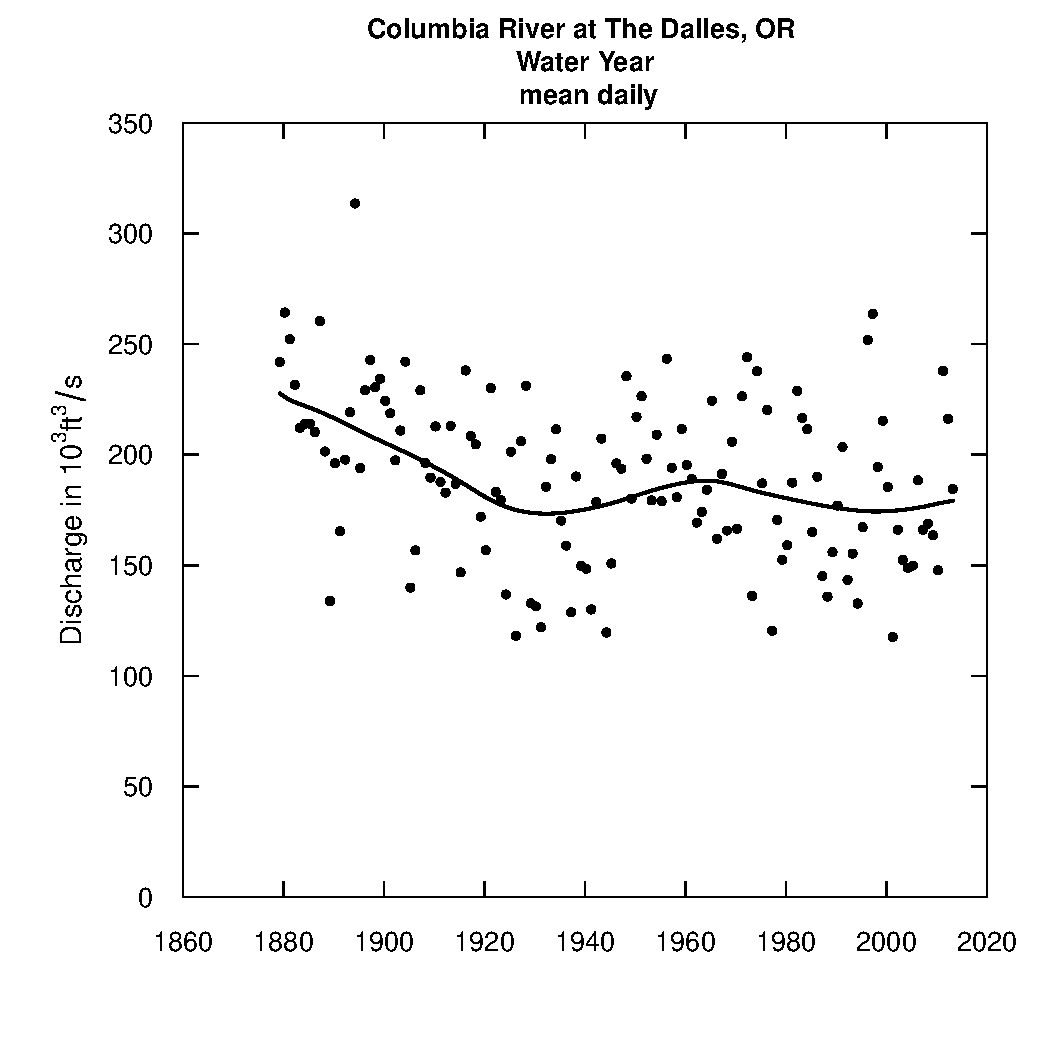
\includegraphics[width=.5\linewidth,height=.5\linewidth]{figure/plotSingleandSD1} }
\subfloat[plotSDLogQ()\label{fig:plotSingleandSD2}]{
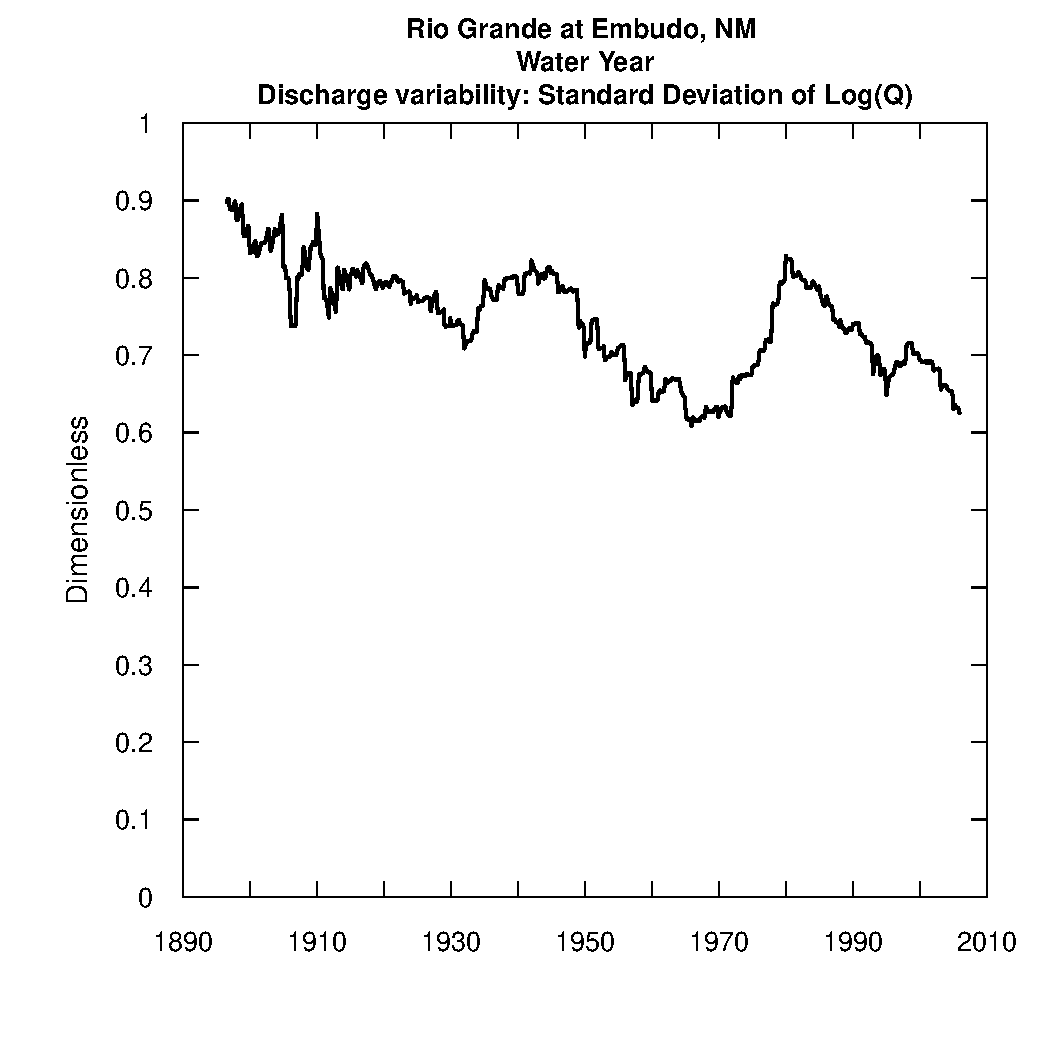
\includegraphics[width=.5\linewidth,height=.5\linewidth]{figure/plotSingleandSD2} }\caption[Discharge statistics]{Discharge statistics\label{fig:plotSingleandSD}}
\end{figure}


\end{knitrout}


Figure \ref{fig:plotFour}:
\begin{knitrout}
\definecolor{shadecolor}{rgb}{0.969, 0.969, 0.969}\color{fgcolor}\begin{kframe}
\begin{alltt}
\hlfunctioncall{plotFour}(qUnit=3)
\end{alltt}
\end{kframe}\begin{figure}[]

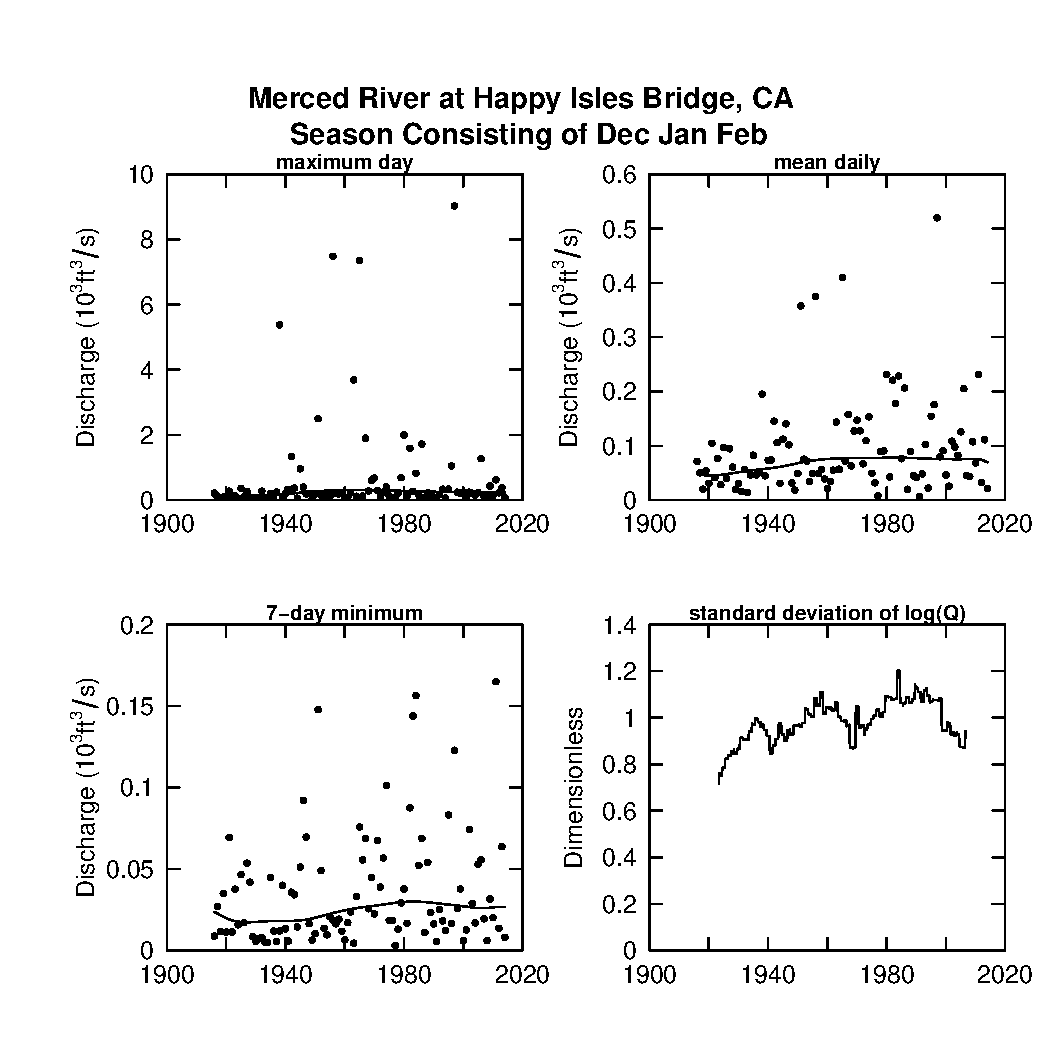
\includegraphics[width=1\linewidth,height=1\linewidth]{figure/plotFour} \caption[plotFour(qUnit=3)]{plotFour(qUnit=3)\label{fig:plotFour}}
\end{figure}


\end{knitrout}


Figure \ref{fig:plotFourStats}:
\begin{knitrout}
\definecolor{shadecolor}{rgb}{0.969, 0.969, 0.969}\color{fgcolor}\begin{kframe}
\begin{alltt}
\hlfunctioncall{plotFourStats}(qUnit=3)
\end{alltt}
\end{kframe}\begin{figure}[]

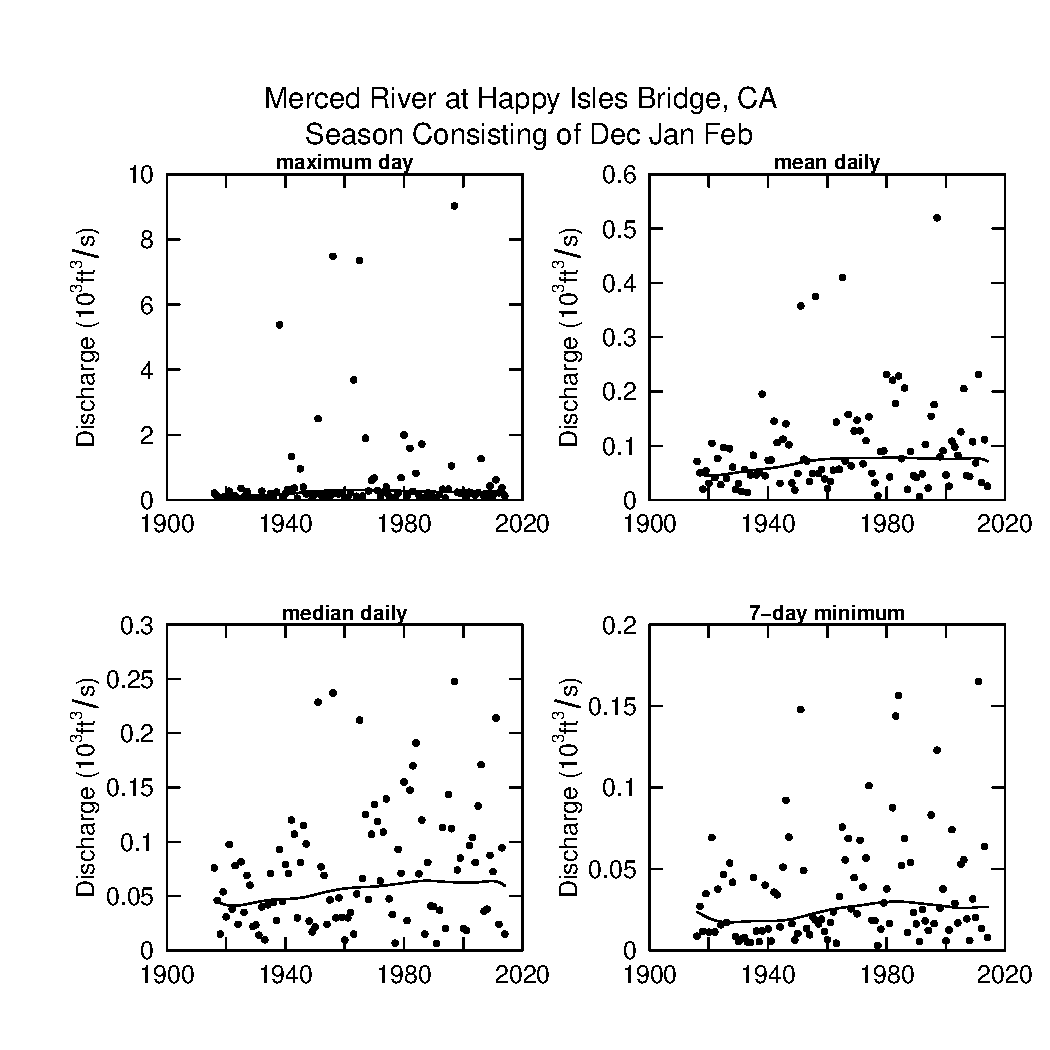
\includegraphics[width=1\linewidth,height=1\linewidth]{figure/plotFourStats} \caption[plotFourStats(qUnit=3)]{plotFourStats(qUnit=3)\label{fig:plotFourStats}}
\end{figure}


\end{knitrout}



\FloatBarrier

The simplest way to look at these time series is with the function plotFlowSingle. The statistic index (istat) must be defined, but other input arguements can defined. To see a list of these optional arguments and other information about the function, type ?plotFlowSingle in the R console. All of the graphs in plotFlowSingle, plotFourStats, and all but one of the graphs in plotFour, show both the individual annual values of the selected flow statistic (e.g. the annual mean or 7-day minimum), but they also show a curve that is a smooth fit to those data.  The curve is a LOWESS (locally weighted scatterplot smooth).  The algorithm for computing it is provided in \cite{HirschV}:\url{http://pubs.usgs.gov/sir/2012/5151/}  (pages 6 and 7).  The default is that they are smoothed with a "half-window width" of 30 years and the smoothing is performed on the log discharge values.  The smoothing window is a user-defined option. 

plotSDLogQ produces a graphic of the running standard deviation of the log of daily discharge over time.  The idea is to get some idea of how variability of daily discharge is changing over time.  By using the standard deviation of the log discharge the statistic becomes dimensionless.  It also means that it is a way of looking at variability quite aside from average values, so, in the case of a system where discharge might be increasing over a period of years, this provides a way of looking at the variability relative to that changing mean value.  It is much like a coefficient of variation, but it has sample properties that make it a smoother measure of variability.  There are often comments about how things like urbanization or enhanced greenhouse gases in the atmosphere are bringing about an increase in variability, this is one way to explore that idea. plotFour, plotFourStats, and plot15 are all designed to plot several graphs from the other functions all in a single figure. 

Here is an example of looking at mean daily streamflow for the full water year and then looking at mean daily streamflow for the winter season only.  The site being considered is the Merced River at Happy Isles Bridge in Yosemite National Park in California.  First, we can look at the mean daily streamflow for the full year (after having read in the data and metadata):

\begin{knitrout}
\definecolor{shadecolor}{rgb}{0.969, 0.969, 0.969}\color{fgcolor}\begin{kframe}
\begin{alltt}
sta<-\hlstring{"11264500"}
Daily <-\hlfunctioncall{getDVData}(sta,\hlstring{"00060"},StartDate=\hlstring{""},EndDate=\hlstring{""})
\end{alltt}
\begin{verbatim}
## There are  35728 data points, and  35728 days.
\end{verbatim}
\begin{alltt}
INFO <- \hlfunctioncall{getMetaData}(sta,\hlstring{""},interactive=FALSE)
INFO$shortName <- \hlstring{"Merced River, CA"}
INFO <- \hlfunctioncall{setPA}()
annualSeries <- \hlfunctioncall{makeAnnualSeries}()
\hlfunctioncall{plotFlowSingle}(istat=5)

INFO<-\hlfunctioncall{setPA}(paStart=12,paLong=3)
annualSeries<-\hlfunctioncall{makeAnnualSeries}()
\hlfunctioncall{plotFlowSingle}(istat=5)
\end{alltt}
\end{kframe}\begin{figure}[]
\subfloat[Water Year\label{fig:Merced1}]{
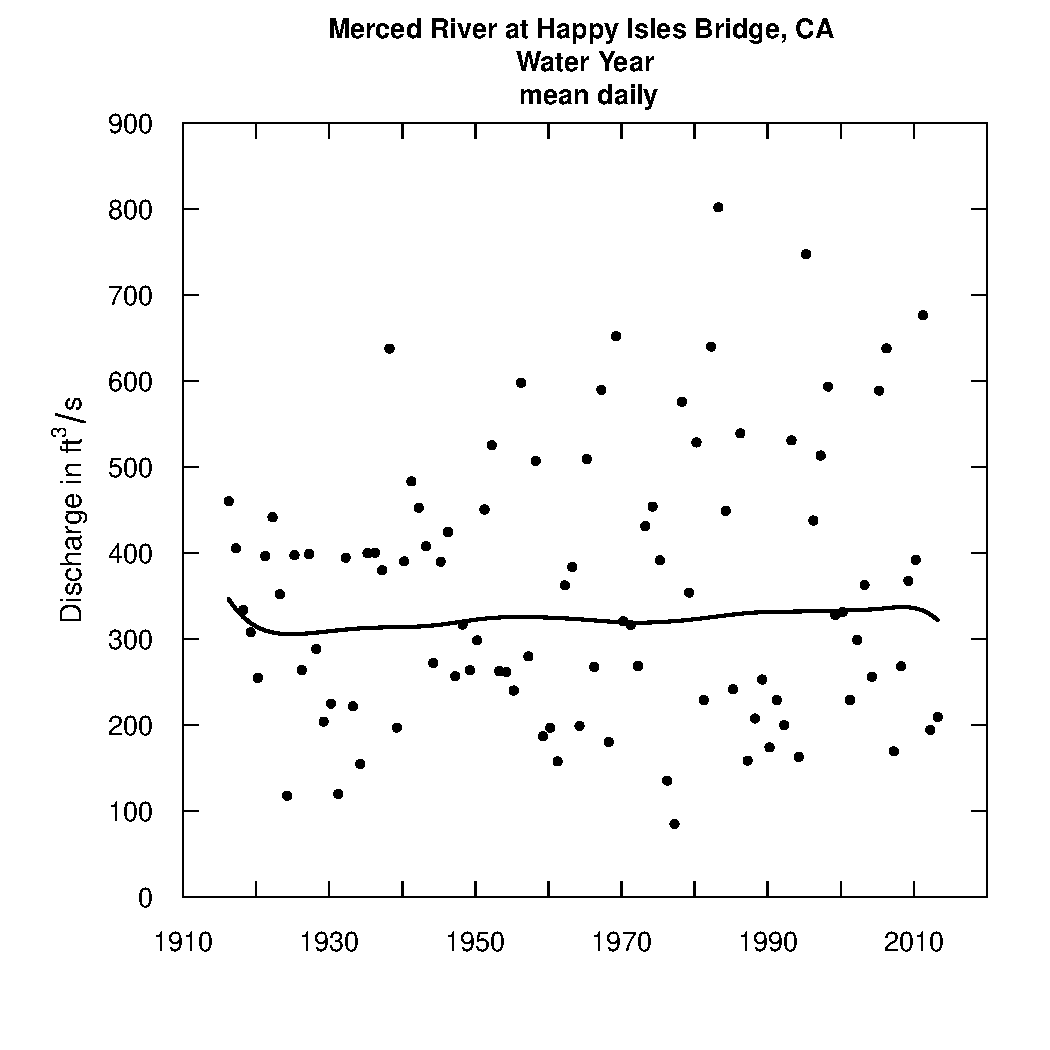
\includegraphics[width=.5\linewidth,height=.5\linewidth]{figure/Merced1} }
\subfloat[Dec-Feb\label{fig:Merced2}]{
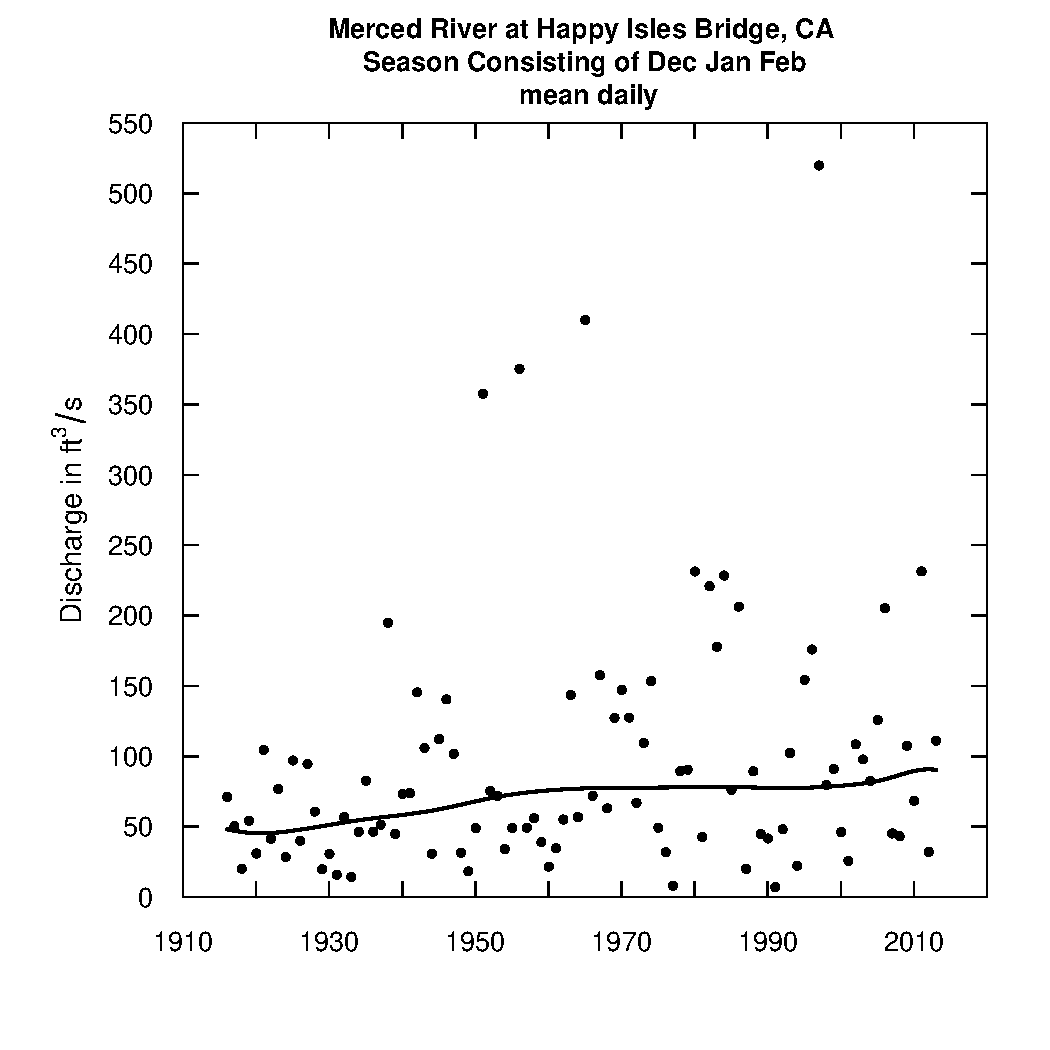
\includegraphics[width=.5\linewidth,height=.5\linewidth]{figure/Merced2} }\caption[Merced River Winter Trend]{Merced River Winter Trend\label{fig:Merced}}
\end{figure}


\end{knitrout}


The two figures produced are shown below.  What they show us is that on an annual basis there is very little indication of a long-term trend in mean streamflow, but for the winter months there is a pretty strong indication of an upward trend.  This could well be related to the climate warming in the Sierra Nevada, resulting in a general increase in the ratio of rain to snow in the winter and more thawing events.

plotQTimeDaily is simply a time series plot of discharge.  But, it is most suited for showing events above some discharge threshold.  In the simplest case, it can plot the entire record, but given the line weight and use of an arithmetic scale it will primarily provide a visual focus on the higher values.

\begin{knitrout}
\definecolor{shadecolor}{rgb}{0.969, 0.969, 0.969}\color{fgcolor}\begin{kframe}
\begin{alltt}
sta<-\hlstring{"05474500"}
Daily <-\hlfunctioncall{getDVData}(sta,\hlstring{"00060"},StartDate=\hlstring{""},EndDate=\hlstring{""})
\end{alltt}
\begin{verbatim}
## There are  49428 data points, and  49428 days.
\end{verbatim}
\begin{alltt}
INFO <- \hlfunctioncall{getMetaData}(sta,\hlstring{""},interactive=FALSE)
INFO$shortName <- \hlstring{"Mississippi River at Keokuk Iowa"}
INFO <- \hlfunctioncall{setPA}()

\hlfunctioncall{plotQTimeDaily}(startYear=1870,endYear=2020,qUnit=3,qLower=300)
\end{alltt}
\end{kframe}\begin{figure}[]

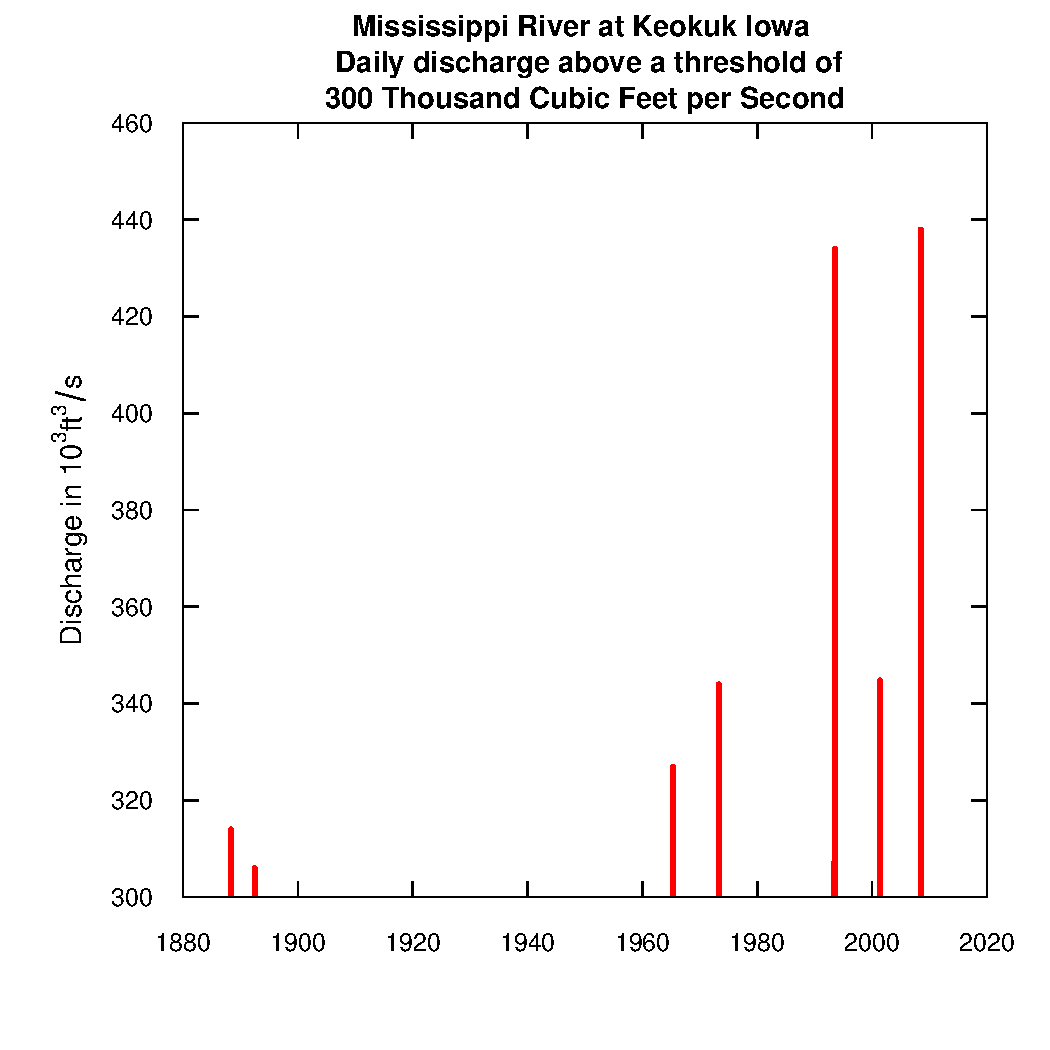
\includegraphics[width=1\linewidth,height=1\linewidth]{figure/Mississippi} \caption[Mississippi River at Keokuk Iowa]{Mississippi River at Keokuk Iowa\label{fig:Mississippi}}
\end{figure}


\end{knitrout}


The example shown here illustrates a very long record and the long gap of more than 60 years of no flows above 300,000 ft\verb|^|3/s, followed by the last 50 years with at least 5 events above that threshold. plotQTimeDaily requires startYear and endYear, along with some other optional arguements (see ?plotQTimeDaily for more details).

\FloatBarrier

%------------------------------------------------------------ 
\subsection{Table Options}
\label{sec:tableOptions}
%------------------------------------------------------------ 
Sometimes easier to consider the results in table formats rather than graphically. Similar to the function plotFlowSingle, the printSeries will print the requested flow statistics (Table \ref{table:istat}). A small sample of the output is printed below.


\begin{knitrout}
\definecolor{shadecolor}{rgb}{0.969, 0.969, 0.969}\color{fgcolor}\begin{kframe}
\begin{alltt}
\hlfunctioncall{printSeries}(istat=3, qUnit=3)
\end{alltt}
\end{kframe}
\end{knitrout}


\begin{verbatim}
Mississippi River at Keokuk Iowa
 Water Year
    30-day minimum
    Thousand Cubic Feet per Second
   year   annual   smoothed
           value    value
   1879     22.6     30.1
   1880     31.7     28.7
   1881     23.0     27.5
...
   2011     51.0     32.4
   2012     34.3     32.1
   2013     16.2     31.8
\end{verbatim}

Another way to look at the results is to consider how much the smoothed values change between various pairs of years.  These changes can be represented in four different ways.  
\begin{itemize}
  \item As a change between the first and last year of the pair, expressed in the flow units selected.
  \item As a change between the first and last year of the pair, expressed as a percentage of the value in the first year
  \item As a slope between the first and last year of the pair, expressed in terms of the flow units per year.
  \item As a slope between the first and last year of the pair, expressed as a percentage change per year (a percentage based on the value in the first year).
\end{itemize}

There is another argument that can be very useful in this function: yearPoints.  In the default case, the set of years that are compared are at 5 year intervals along the whole data set.  If the data set was quite long this can be a daunting number of comparisons.  For example, in an 80 year record, there would be 136 such pairs. Instead, we could look at changes for every 20 years starting in 1930: 


\begin{knitrout}
\definecolor{shadecolor}{rgb}{0.969, 0.969, 0.969}\color{fgcolor}\begin{kframe}
\begin{alltt}
annualSeries <- \hlfunctioncall{makeAnnualSeries}()
\hlfunctioncall{tableFlowChange}(istat=3, qUnit=3,yearPoints=\hlfunctioncall{c}(1890,1950,2010))
\end{alltt}
\begin{verbatim}
## 
##    Mississippi River at Keokuk Iowa
##    Water Year
##     30-day minimum 
## 
##              Streamflow Trends
##    time span          change        slope       change        slope
##                       10^3 cfs 10^3 cfs /yr         %         %/yr
##  1890  to  1950         0.54       0.0091          2.4         0.04
##  1890  to  2010          9.8        0.082           43         0.36
##  1950  to  2010          9.3         0.15           40         0.66
\end{verbatim}
\end{kframe}
\end{knitrout}


See Appendix \ref{app:createWordTable} for instructions on converting an R dataframe to a table in Microsoft. 

\FloatBarrier


%------------------------------------------------------------ 
\section{Summary of Water Quality Data (without using WRTDS)}
\label{sec:wqa}
%------------------------------------------------------------ 
\FloatBarrier

Before running the WRTDS model, it is very helpful to take a look at the measured data in a graphical way to understand its behavior and to identify things that might be errors in the data set or learn about the temporal distribution of the data (identify gaps) prior to running the model.  It is always best to clear up these issues before moving forward.

We will now use the Choptank River at Greensboro, MD as our example case. The Choptank River is a small tributary of the Chesapeake Bay. Inorganic nitrogen (nitrate and nitrite) has been measured from 1979 onward. First, we need to get the streamflow and nitrate data into R, then use the mergeReport function to associate flow with the discrete measured water quality data. Before the data can be graphed or entered into any of the WRTDS analysis the discharge data must be brought into the Sample dataframe.  This is done with the mergeReport function which does this merger of the discharge information and also provides a compact report about some major features of the data set.

\begin{knitrout}
\definecolor{shadecolor}{rgb}{0.969, 0.969, 0.969}\color{fgcolor}\begin{kframe}
\begin{alltt}
siteID <- \hlstring{"01491000"} #Choptank River at Greensboro, MD
startDate <- \hlstring{"1979-10-01"}
endDate <- \hlstring{"2011-09-30"}
param<-\hlstring{"00631"}
Daily <- \hlfunctioncall{getDVData}(siteID,\hlstring{"00060"},startDate,endDate)
INFO<- \hlfunctioncall{getMetaData}(siteID,param,interactive=FALSE)
INFO$shortName <- \hlstring{"Choptank River"}

Sample <- \hlfunctioncall{getSampleData}(siteID,param,startDate,endDate)
Sample <- \hlfunctioncall{mergeReport}()
\end{alltt}
\end{kframe}
\end{knitrout}






%------------------------------------------------------------ 
\subsection{Plotting Options}
\label{sec:plotOptionsWQ}
%------------------------------------------------------------ 
\FloatBarrier

This section will give examples of the available plots appropriate for analyzing the data prior to performing a WRTDS analysis. The plots here will use the default variable input options.  For any function, you can get a complete list of input variables (as described in the previous section) in a help file by typing a ? before the function name in the R console. See Appendix \ref{sec:wqVariables} for information on the available input variables for these plotting functions. Also, the complete EGRET manual has more detailed information for each plot type (\href{https://github.com/USGS-R/EGRET/raw/Documentation/EGRET%2Bmanual_4.doc}{link to download}).

One note about any of the plotting functions that show the sample data:  If a value in the data set is a non-detect. Then it is displayed on a graph as a vertical line.  The top of the line is the reporting limit and the bottom is either zero, or if the graph is plotting log concentration values, the minimum value on the y-axis.  This line is an 'honest' representation of what we know about that observation and doesn't involve us using a statistical model to fill in what we don't know. 

Figure \ref{fig:plotBoxes}:
\begin{knitrout}
\definecolor{shadecolor}{rgb}{0.969, 0.969, 0.969}\color{fgcolor}\begin{kframe}
\begin{alltt}
\hlfunctioncall{boxConcMonth}()
\hlfunctioncall{boxQTwice}(qUnit=1)
\end{alltt}
\end{kframe}\begin{figure}[]
\subfloat[boxConcMonth()\label{fig:plotBoxes1}]{
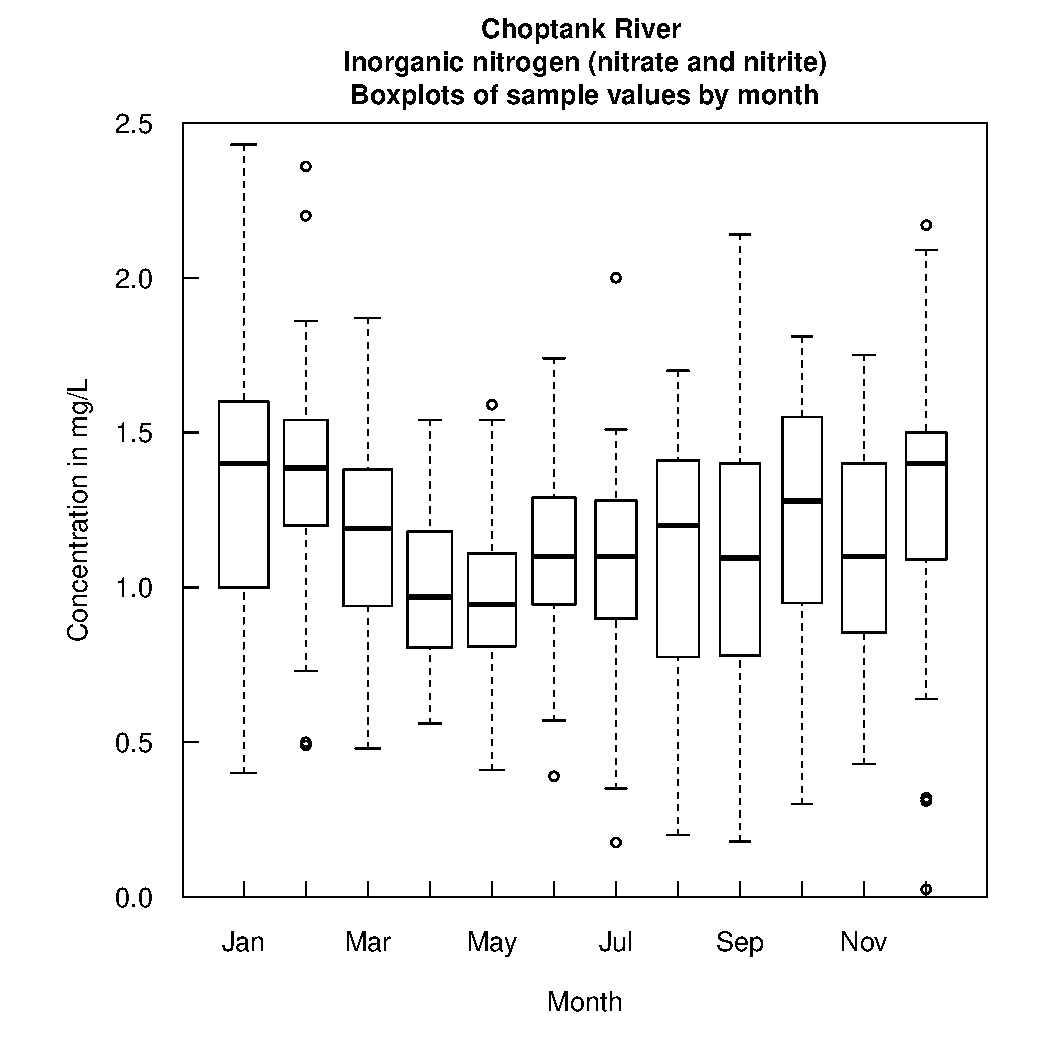
\includegraphics[width=.5\linewidth,height=.5\linewidth]{figure/plotBoxes1} }
\subfloat[boxQTwice(qUnit=1)\label{fig:plotBoxes2}]{
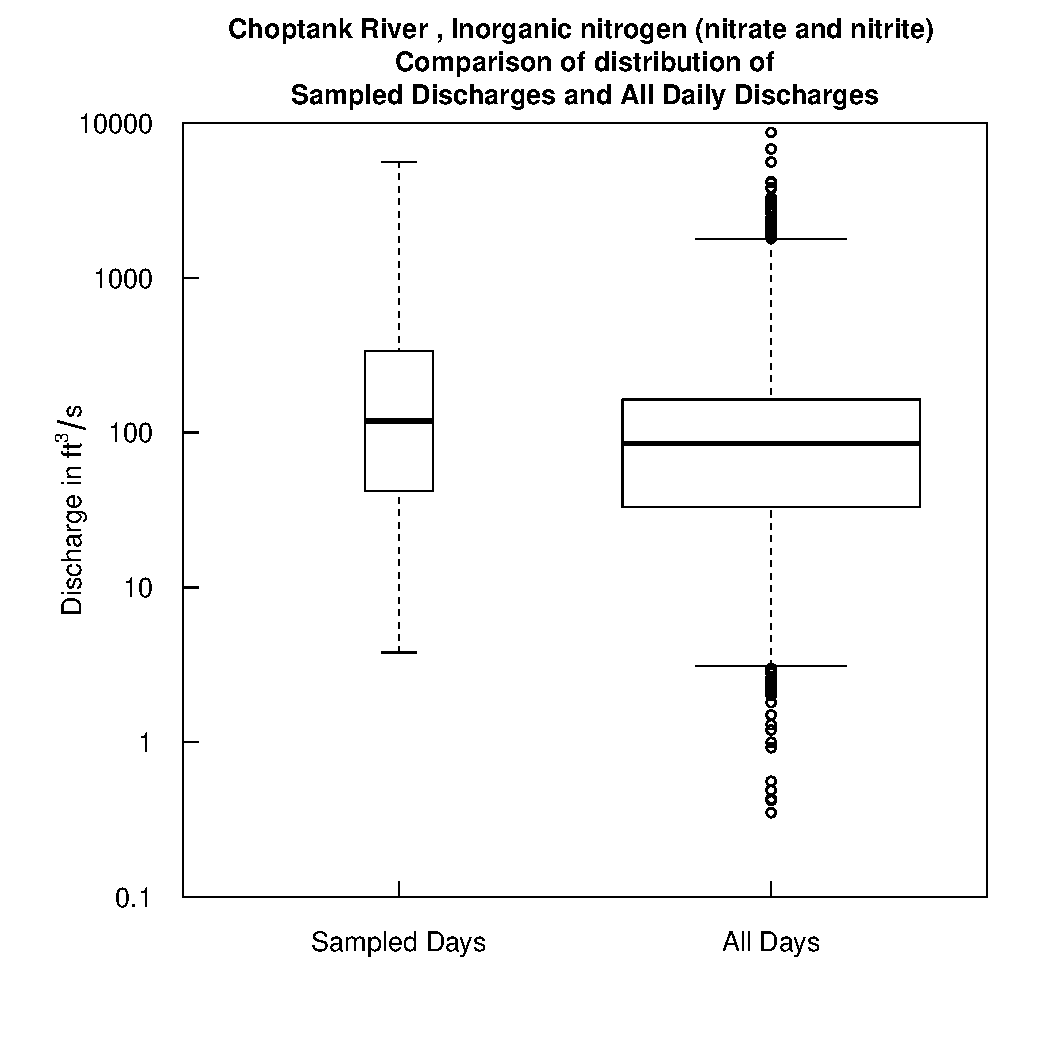
\includegraphics[width=.5\linewidth,height=.5\linewidth]{figure/plotBoxes2} }\caption[Concentration box plots]{Concentration box plots\label{fig:plotBoxes}}
\end{figure}


\end{knitrout}


Note that the statistics to create the boxplot in boxQTwice are performed after the data is log-transformed.

Figure \ref{fig:plotConcTime}:
\begin{knitrout}
\definecolor{shadecolor}{rgb}{0.969, 0.969, 0.969}\color{fgcolor}\begin{kframe}
\begin{alltt}
\hlfunctioncall{plotConcTime}()
\hlfunctioncall{plotLogConcTime}()
\end{alltt}
\end{kframe}\begin{figure}[]
\subfloat[plotConcTime()\label{fig:plotConcTime1}]{
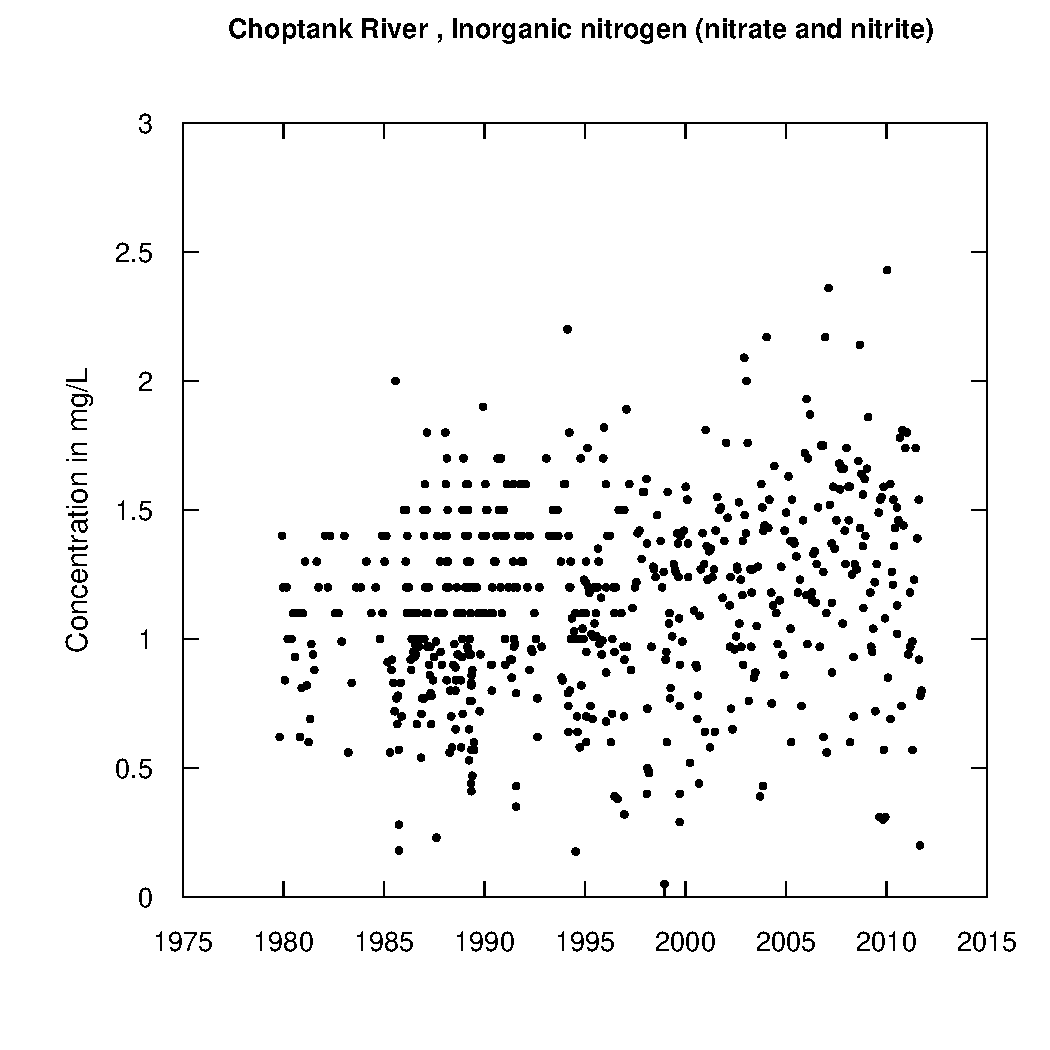
\includegraphics[width=.5\linewidth,height=.5\linewidth]{figure/plotConcTime1} }
\subfloat[plotLogConcTime()\label{fig:plotConcTime2}]{
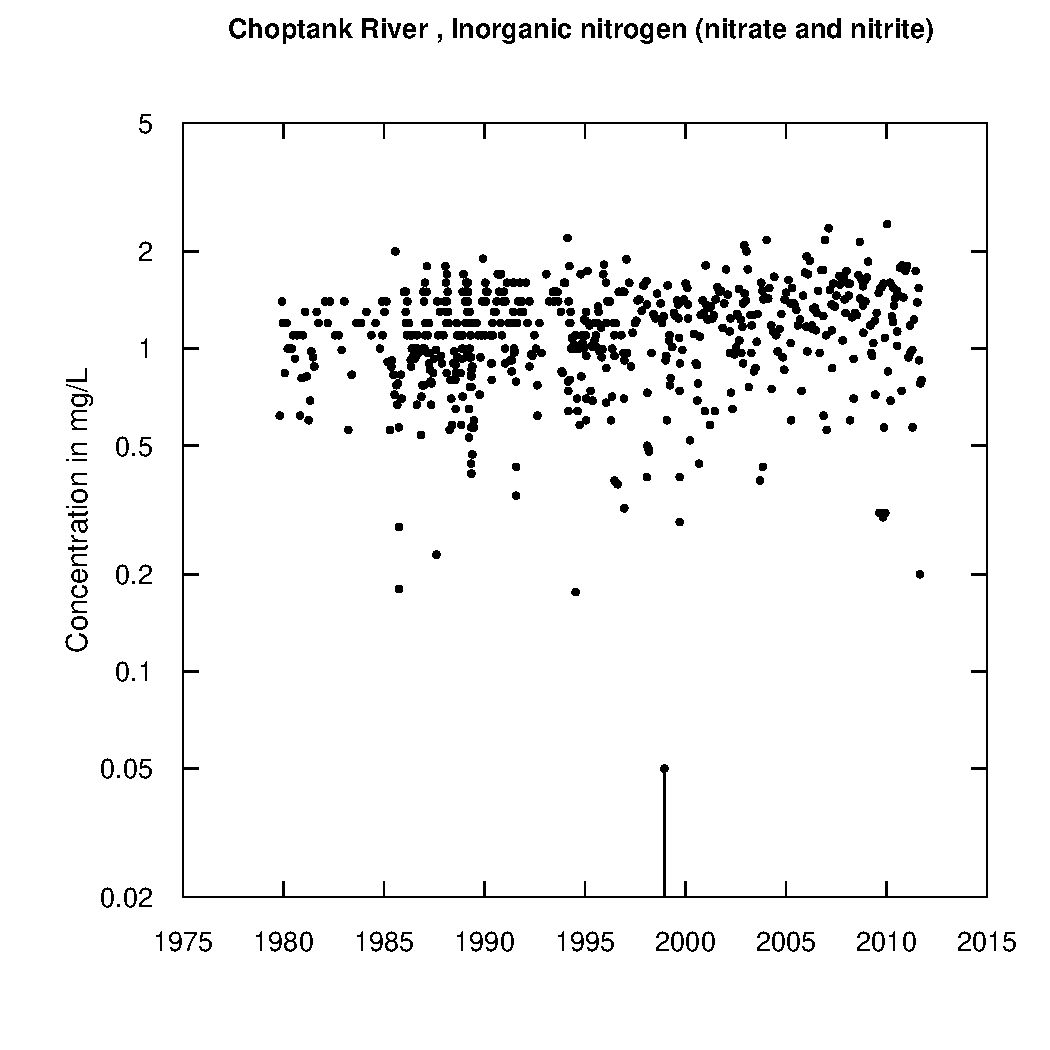
\includegraphics[width=.5\linewidth,height=.5\linewidth]{figure/plotConcTime2} }\caption[Concentration vs time]{Concentration vs time\label{fig:plotConcTime}}
\end{figure}


\end{knitrout}


Figure \ref{fig:plotConcQ}:
\begin{knitrout}
\definecolor{shadecolor}{rgb}{0.969, 0.969, 0.969}\color{fgcolor}\begin{kframe}
\begin{alltt}
\hlfunctioncall{plotConcQ}(qUnit=1)
\hlfunctioncall{plotLogConcQ}(qUnit=1)
\end{alltt}
\end{kframe}\begin{figure}[]
\subfloat[plotConcQ(qUnit=1)\label{fig:plotConcQ1}]{
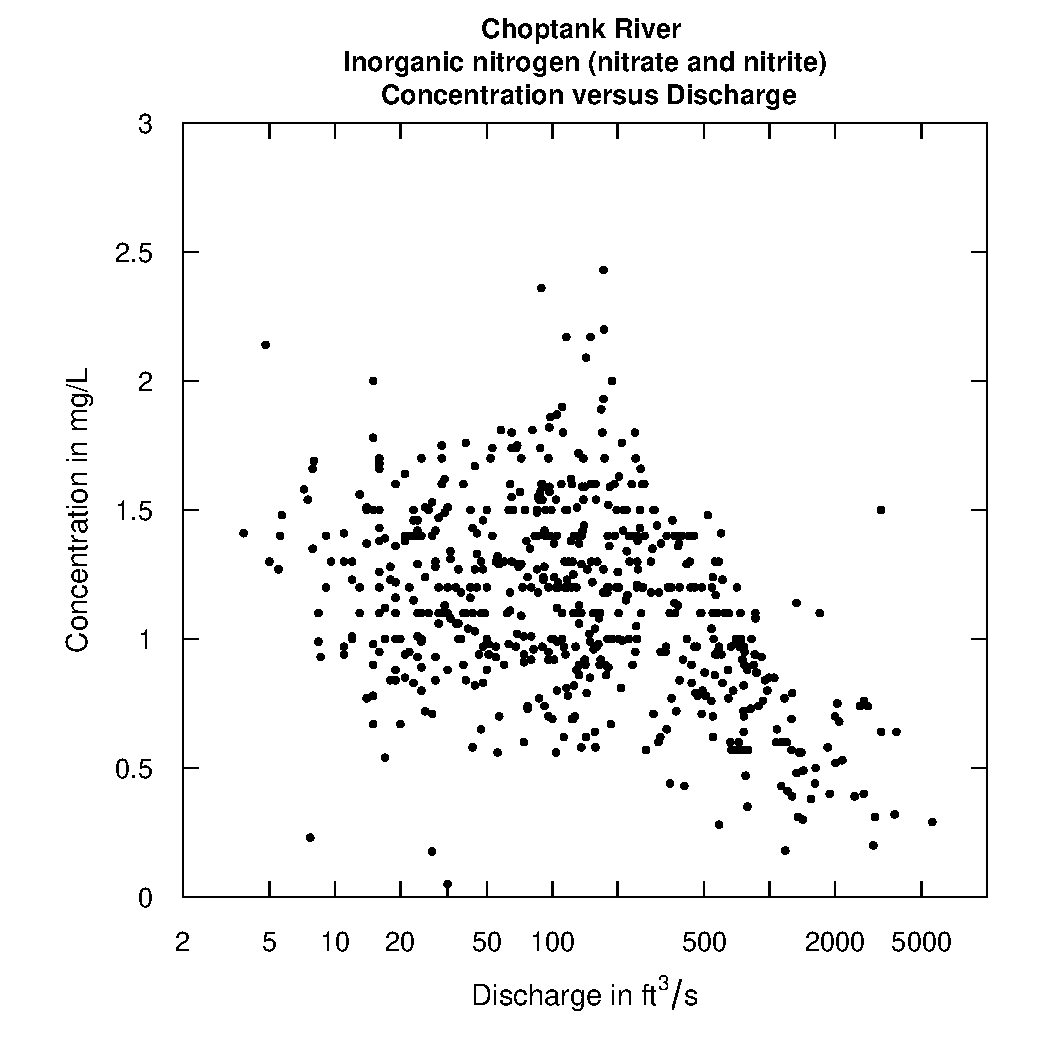
\includegraphics[width=.5\linewidth,height=.5\linewidth]{figure/plotConcQ1} }
\subfloat[plotLogConcQ(qUnit=1)\label{fig:plotConcQ2}]{
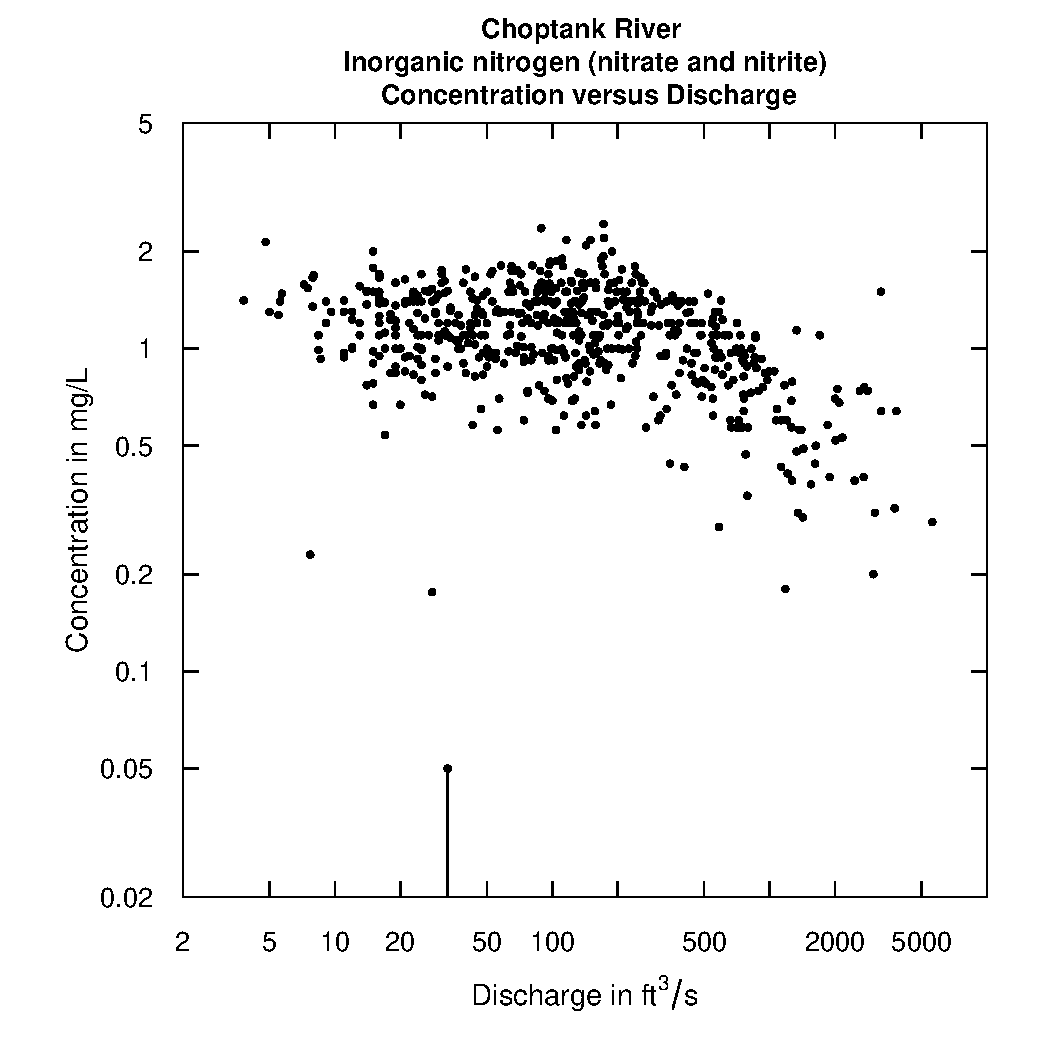
\includegraphics[width=.5\linewidth,height=.5\linewidth]{figure/plotConcQ2} }\caption[Concentration vs discharge]{Concentration vs discharge\label{fig:plotConcQ}}
\end{figure}


\end{knitrout}


Figure \ref{fig:plotLogConcQ}:
\begin{knitrout}
\definecolor{shadecolor}{rgb}{0.969, 0.969, 0.969}\color{fgcolor}\begin{kframe}
\begin{alltt}
\hlfunctioncall{plotLogFluxQ}(qUnit=1)
\end{alltt}
\end{kframe}\begin{figure}[]

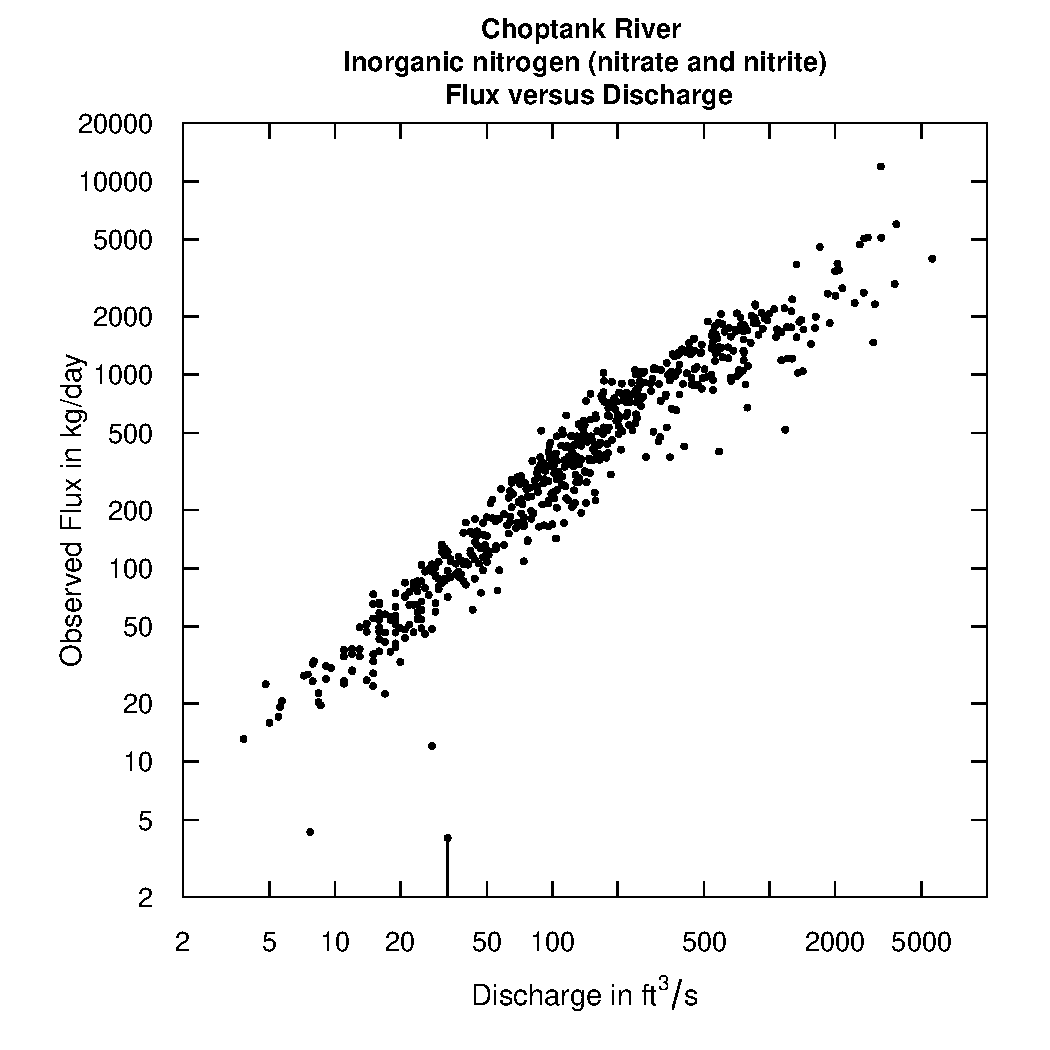
\includegraphics[width=.5\linewidth,height=.5\linewidth]{figure/plotLogConcQ} \caption[plotLogFluxQ(qUnit=1)]{plotLogFluxQ(qUnit=1)\label{fig:plotLogConcQ}}
\end{figure}


\end{knitrout}


Figure \ref{fig:multiPlotDataOverview}:
\begin{knitrout}
\definecolor{shadecolor}{rgb}{0.969, 0.969, 0.969}\color{fgcolor}\begin{kframe}
\begin{alltt}
\hlfunctioncall{multiPlotDataOverview}(qUnit=1)
\end{alltt}
\end{kframe}\begin{figure}[]

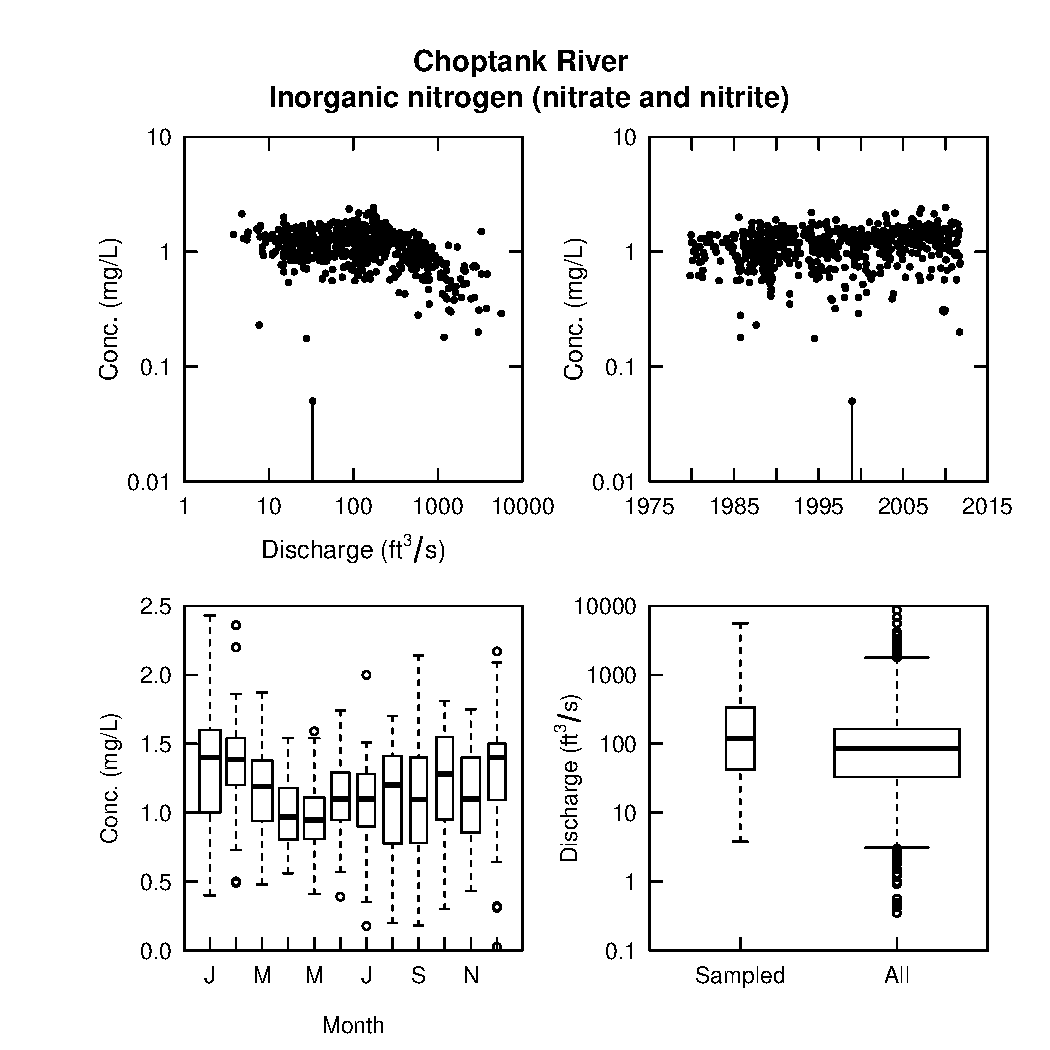
\includegraphics[width=1\linewidth,height=1\linewidth]{figure/multiPlotDataOverview} \caption[multiPlotDataOverview(qUnit=1)]{multiPlotDataOverview(qUnit=1)\label{fig:multiPlotDataOverview}}
\end{figure}


\end{knitrout}


\FloatBarrier

%------------------------------------------------------------ 
\subsection{Extending Plots Past Defaults}
\label{sec:extendedPlots}
%------------------------------------------------------------ 

\FloatBarrier

The basic plotting options were shown in the previous section.  This section demonstrates some ideas on how to extend the capabilities of the EGRET plots. EGRET plots use R's base plotting options. Default graphical parameters (see ?mar) and plot parameters were chosen, but all can be overridden. Additionally, features can be added to a plot after calling the plot function. To change the plot margins, set the argument customPar to TRUE.

Figure \ref{fig:plotLogConcQComparison}:
\begin{knitrout}
\definecolor{shadecolor}{rgb}{0.969, 0.969, 0.969}\color{fgcolor}\begin{kframe}
\begin{alltt}
\hlfunctioncall{plotLogConcQ}()
\hlfunctioncall{par}(mar=\hlfunctioncall{c}(8,8,8,8))

\hlfunctioncall{plotLogConcQ}(customPar=TRUE,col=\hlstring{"blue"},cex=1.1,
             cex.axis=1.4,cex.main=1.5,cex.lab=1.2,pch=18,lwd=2)
\hlfunctioncall{grid}()
\hlfunctioncall{legend}(4.5,.1,\hlstring{"Choptank Nitrogen"}, pch=18, col=\hlstring{"blue"},bg=\hlstring{"white"})
\end{alltt}
\end{kframe}\begin{figure}[]
\subfloat[Default\label{fig:plotLogConcQComparison1}]{
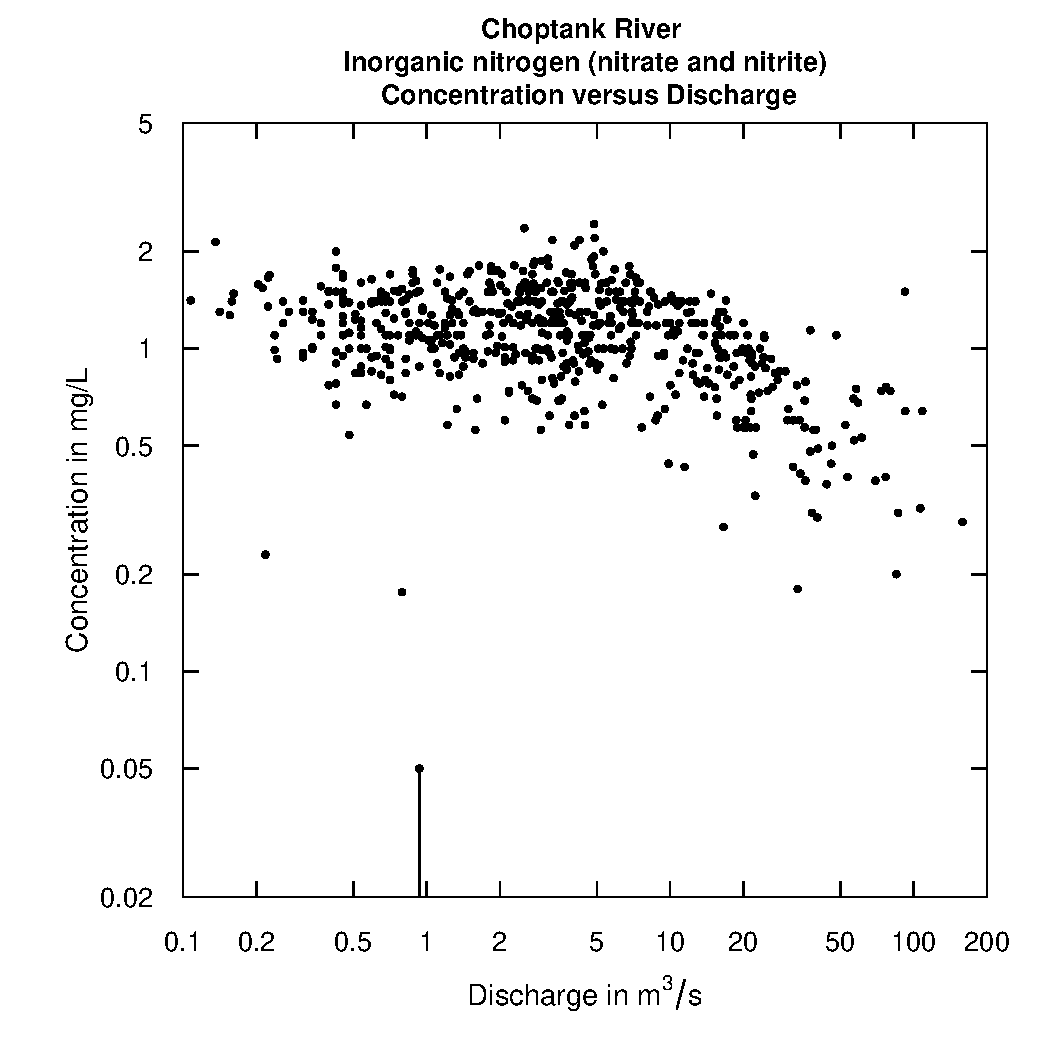
\includegraphics[width=.5\linewidth,height=.5\linewidth]{figure/plotLogConcQComparison1} }
\subfloat[Modified\label{fig:plotLogConcQComparison2}]{
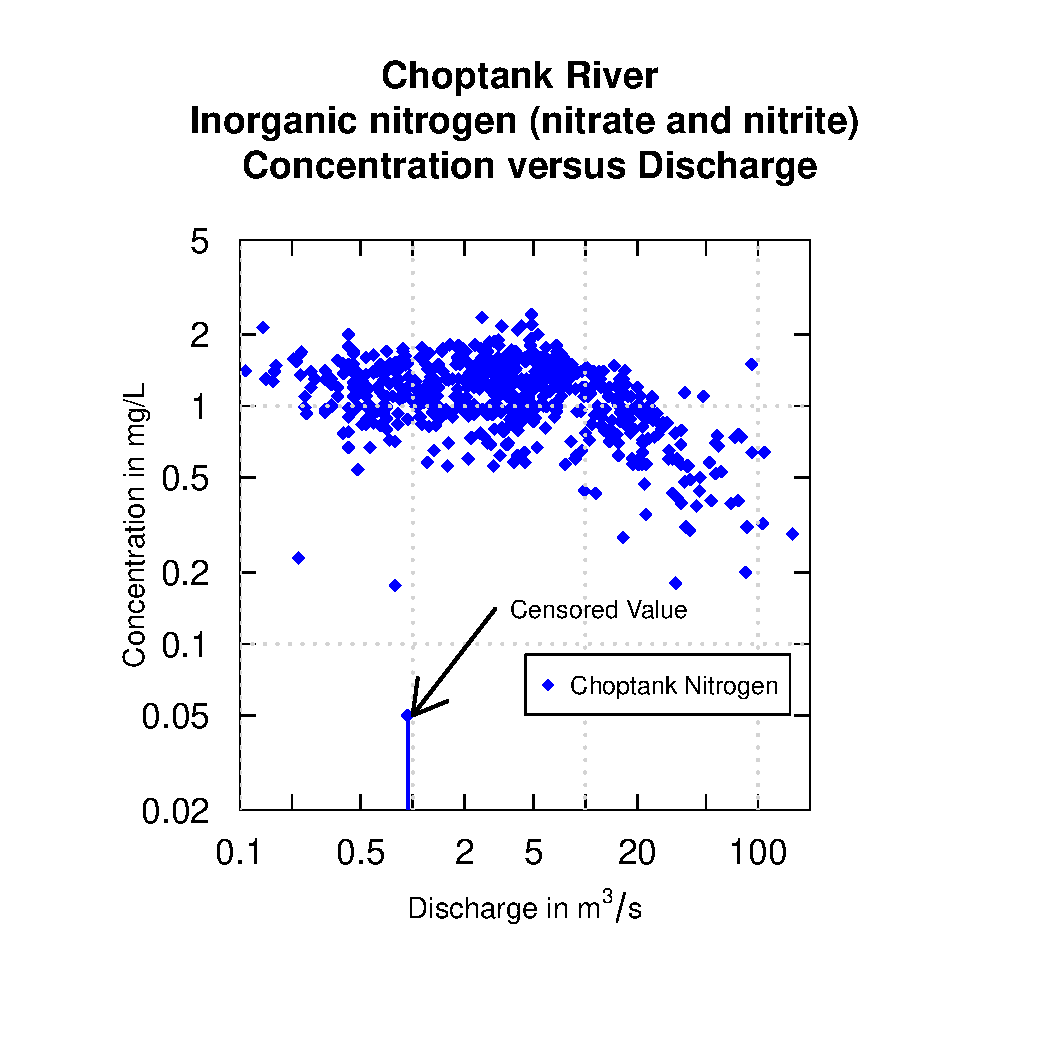
\includegraphics[width=.5\linewidth,height=.5\linewidth]{figure/plotLogConcQComparison2} }\caption[Modified plotLogConcQ]{Modified plotLogConcQ\label{fig:plotLogConcQComparison}}
\end{figure}


\end{knitrout}


Figure \ref{fig:plot-fascinating2}:
\begin{knitrout}
\definecolor{shadecolor}{rgb}{0.969, 0.969, 0.969}\color{fgcolor}\begin{kframe}
\begin{alltt}
\hlcomment{# Adding text to a boxplot:}
bp <- \hlfunctioncall{boxConcMonth}()
\hlfunctioncall{mtext}(\hlfunctioncall{paste}(bp$n, sep = \hlstring{""}), at = \hlfunctioncall{seq_along}(bp$n), 
      line = -1, side = 3, cex=0.75)
\hlfunctioncall{mtext}(\hlstring{"n = "},side=3,line=-1,adj=.01, cex=0.75)
\end{alltt}
\end{kframe}\begin{figure}[]

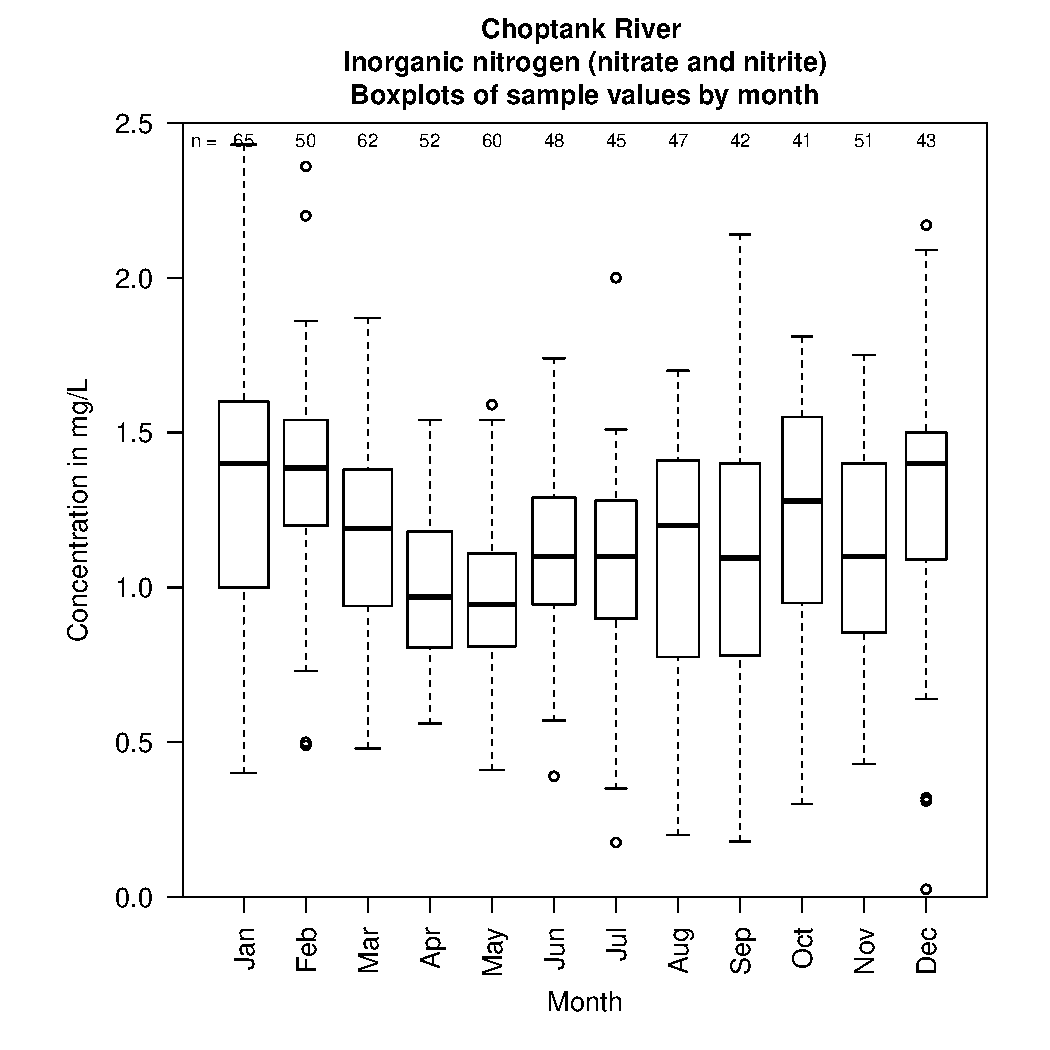
\includegraphics[width=1\linewidth,height=1\linewidth]{figure/plot-fascinating2} \caption[Modified box plot]{Modified box plot\label{fig:plot-fascinating2}}
\end{figure}


\end{knitrout}



\FloatBarrier

%------------------------------------------------------------ 
\subsection{Table Options}
\label{sec:tableOptionsWQ}
%------------------------------------------------------------ 
Another useful tool for checking the data before running the WRTDS estimations is flowDuration. This is a utility function that can help define the flow ranges that we want to explore.  It prints out key points on the flow duration curve.  They are defined for a particular part of the year, although they can be done for the entire year.  

\begin{knitrout}
\definecolor{shadecolor}{rgb}{0.969, 0.969, 0.969}\color{fgcolor}\begin{kframe}
\begin{alltt}
\hlfunctioncall{flowDuration}()
\end{alltt}
\begin{verbatim}
## 
## Flow Duration for Choptank River 
## 
## Flow duration is based on full year
## 
## Discharge units are Cubic Meters per Second
## 
##        min        5%       10%       25%       50%       75%       90%       95%       max
##   9.91e-03  3.40e-01  4.53e-01  9.34e-01  2.41e+00  4.62e+00  8.21e+00  1.31e+01  2.46e+02
\end{verbatim}
\end{kframe}
\end{knitrout}


\FloatBarrier
%------------------------------------------------------------ 
\section{WRTDS Analysis}
\label{sec:wrtds}
%------------------------------------------------------------ 
Weighted Regressions on Time, Discharge and Season (WRTDS) creates a model of long-term trends in river-water quality, seasonal components, and discharge-related components of the behavior of measured water-quality parameters. In this section, we will step though the process require for a WRTDS analysis. The next section (\ref{sec:wrtdsResults}) will detail the available methods to view and evaluate the model results. 

Once you have looked at your data using the tools described in section \ref{sec:wqa}, and have determined there is sufficient representative data, it is time to run the WRTDS model. There are a few inputs that can be defined before running the model (see Appendix \ref{sec:wrtdsInputVariables}).

Assuming you are using the defaults, with dataframes called Daily, Sample, and INFO, the modelEstimation function will run the WRTDS modeling algorithm:

\begin{knitrout}
\definecolor{shadecolor}{rgb}{0.969, 0.969, 0.969}\color{fgcolor}\begin{kframe}
\begin{alltt}
\hlfunctioncall{modelEstimation}()
\end{alltt}
\end{kframe}
\end{knitrout}


This function is slow, and shows the progress in percent complete. See the references and manual for more information. It's important to understand that this is the one function that will globally change your Daily, Sample, and INFO dataframes. It also creates a new matrix: surfaces, and a new dataframe: AnnualResults. It is unusual R programming behavior (and generally considered poor practice), but was chosen to make it easy for the user.

If you wish to change the period of analysis after comleting modelEstimation, there is one more step that needs to happen.  For example, if we want to consider a 3 month season that runs from December through Feburary, we would set paStart = 12 and paLong = 3.  (Note that the period of analysis and the arguments paStart and paLong are introduced at the begining of section \ref{sec:flowHistory} of this document.) After running modelEstimation run the command:

\begin{knitrout}
\definecolor{shadecolor}{rgb}{0.969, 0.969, 0.969}\color{fgcolor}\begin{kframe}
\begin{alltt}
AnnualResults<-\hlfunctioncall{setupYears}(paStart=12,paLong=3)
\end{alltt}
\end{kframe}
\end{knitrout}



Finally, it is a good idea to save your results because of the computational time that has been invested in producing these results. Assuming that you have already created the object savePath, the command is:

\begin{knitrout}
\definecolor{shadecolor}{rgb}{0.969, 0.969, 0.969}\color{fgcolor}\begin{kframe}
\begin{alltt}
savePath <- \hlstring{"C:/Users/ldecicco/WRTDS_Output"}
\hlfunctioncall{saveResults}(savePath) 
\end{alltt}
\end{kframe}
\end{knitrout}


This will now save all of the objects in your workspace. If you have saved workspaces from R versions earlier than 3.0, there will be a warning when opening them in R 3.0 (or \verb|>|). Re-saving the workspace using R 3.0 (or \verb|>|) should get rid of the warning.

Alternatively, you can save the individually generated data in your working directory:

\begin{knitrout}
\definecolor{shadecolor}{rgb}{0.969, 0.969, 0.969}\color{fgcolor}\begin{kframe}
\begin{alltt}
\hlfunctioncall{save}(Daily, file=\hlstring{"Daily.RData"})
\hlfunctioncall{save}(Sample, file=\hlstring{"Sample.RData"})
\hlfunctioncall{save}(INFO, file=\hlstring{"INFO.RData"})
\hlfunctioncall{save}(AnnualResults, file=\hlstring{"AnnualResults.RData"})
\hlfunctioncall{save}(surfaces, file=\hlstring{"surfaces.RData"})
\end{alltt}
\end{kframe}
\end{knitrout}


To load this data later:
\begin{knitrout}
\definecolor{shadecolor}{rgb}{0.969, 0.969, 0.969}\color{fgcolor}\begin{kframe}
\begin{alltt}
\hlfunctioncall{load}(Daily, file=\hlstring{"Daily.RData"})
\hlfunctioncall{load}(Sample, file=\hlstring{"Sample.RData"})
\hlfunctioncall{load}(INFO, file=\hlstring{"INFO.RData"})
\hlfunctioncall{load}(AnnualResults, file=\hlstring{"AnnualResults.RData"})
\hlfunctioncall{load}(surfaces, file=\hlstring{"surfaces.RData"})
\end{alltt}
\end{kframe}
\end{knitrout}



\FloatBarrier

%------------------------------------------------------------ 
\section{WRTDS Results}
\label{sec:wrtdsResults}
%------------------------------------------------------------ 
At this point (after having run modelEstimation) we can start considering how to view the annual averages for the variables that have been calculated.  See Appendix \ref{sec:wrtdsOutputVariables} for common input variables for these functions. Additionally, check the help files (in the R console, type ? followed by the function name).

%------------------------------------------------------------ 
\subsection{Plotting Options}
\label{sec:wrtdsPlotting}
%------------------------------------------------------------ 

\FloatBarrier

Check the help files or manual for more details on the following functions.  See section \ref{app:savingPlots} for information on saving plots.






Figure \ref{fig:plotConcTimeDaily}:
\begin{knitrout}
\definecolor{shadecolor}{rgb}{0.969, 0.969, 0.969}\color{fgcolor}\begin{kframe}
\begin{alltt}
yearStart <- 2008
yearEnd <- 2010

\hlfunctioncall{plotConcTimeDaily}(yearStart, yearEnd)
\hlfunctioncall{plotFluxTimeDaily}(yearStart, yearEnd)
\end{alltt}
\end{kframe}\begin{figure}[]
\subfloat[plotConcTimeDaily(yearStart=2008, yearEnd=2010)\label{fig:plotConcTimeDaily1}]{
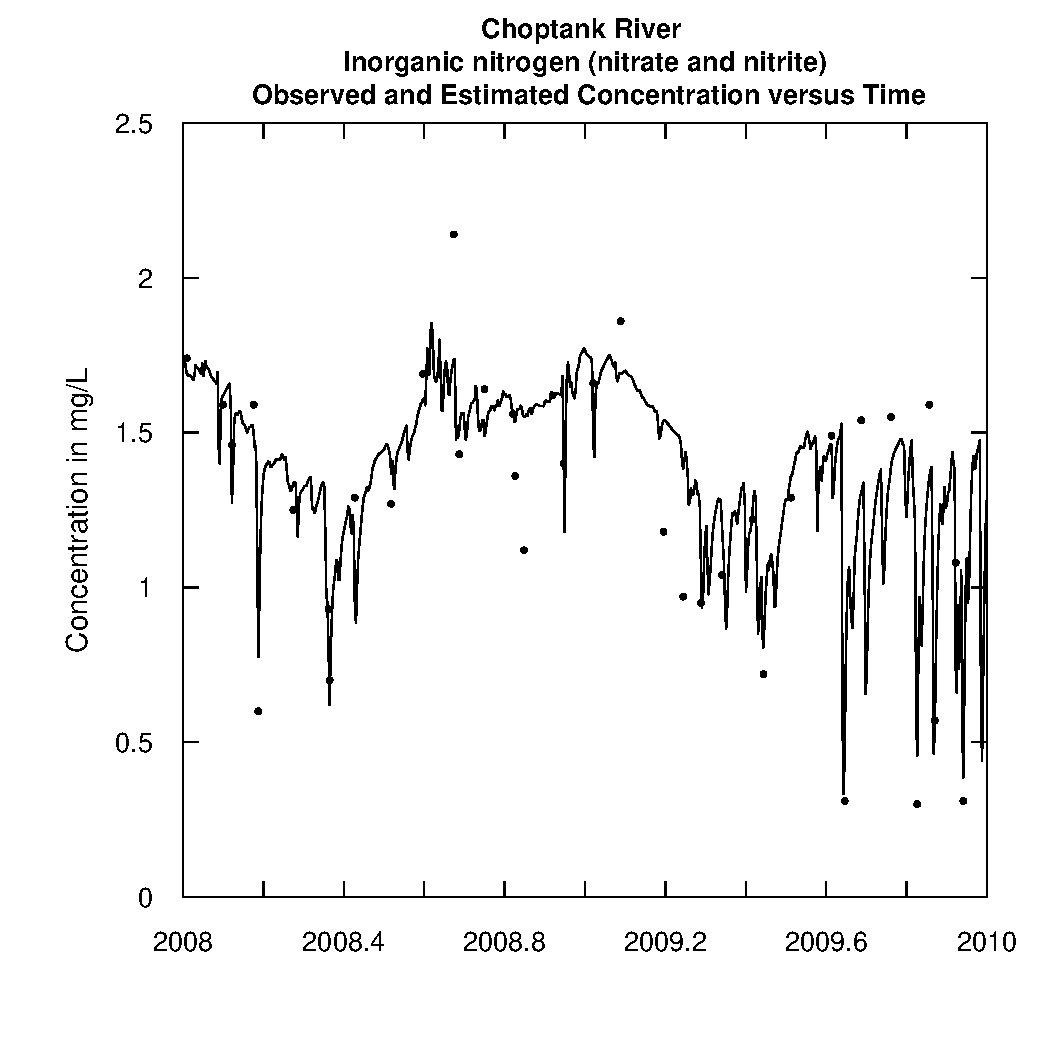
\includegraphics[width=.5\linewidth,height=.5\linewidth]{figure/plotConcTimeDaily1} }
\subfloat[plotFluxTimeDaily(yearStart=2008, yearEnd=2010)\label{fig:plotConcTimeDaily2}]{
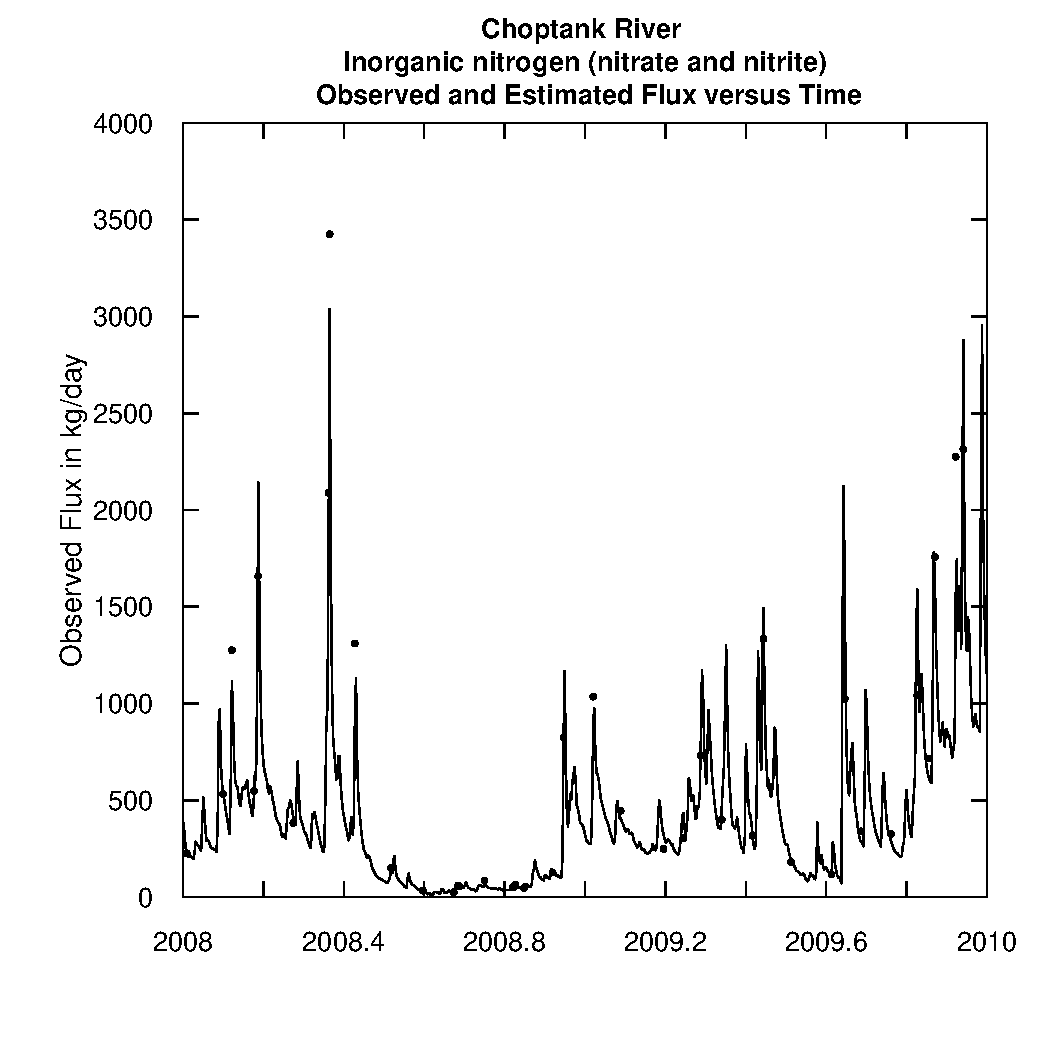
\includegraphics[width=.5\linewidth,height=.5\linewidth]{figure/plotConcTimeDaily2} }\caption[Concentration and flux vs time]{Concentration and flux vs time\label{fig:plotConcTimeDaily}}
\end{figure}


\end{knitrout}


Figure \ref{fig:plotFluxPred}:
\begin{knitrout}
\definecolor{shadecolor}{rgb}{0.969, 0.969, 0.969}\color{fgcolor}\begin{kframe}
\begin{alltt}
\hlfunctioncall{plotConcPred}()
\hlfunctioncall{plotLogConcPred}()
\end{alltt}
\end{kframe}\begin{figure}[]
\subfloat[plotConcPred()\label{fig:plotFluxPred1}]{
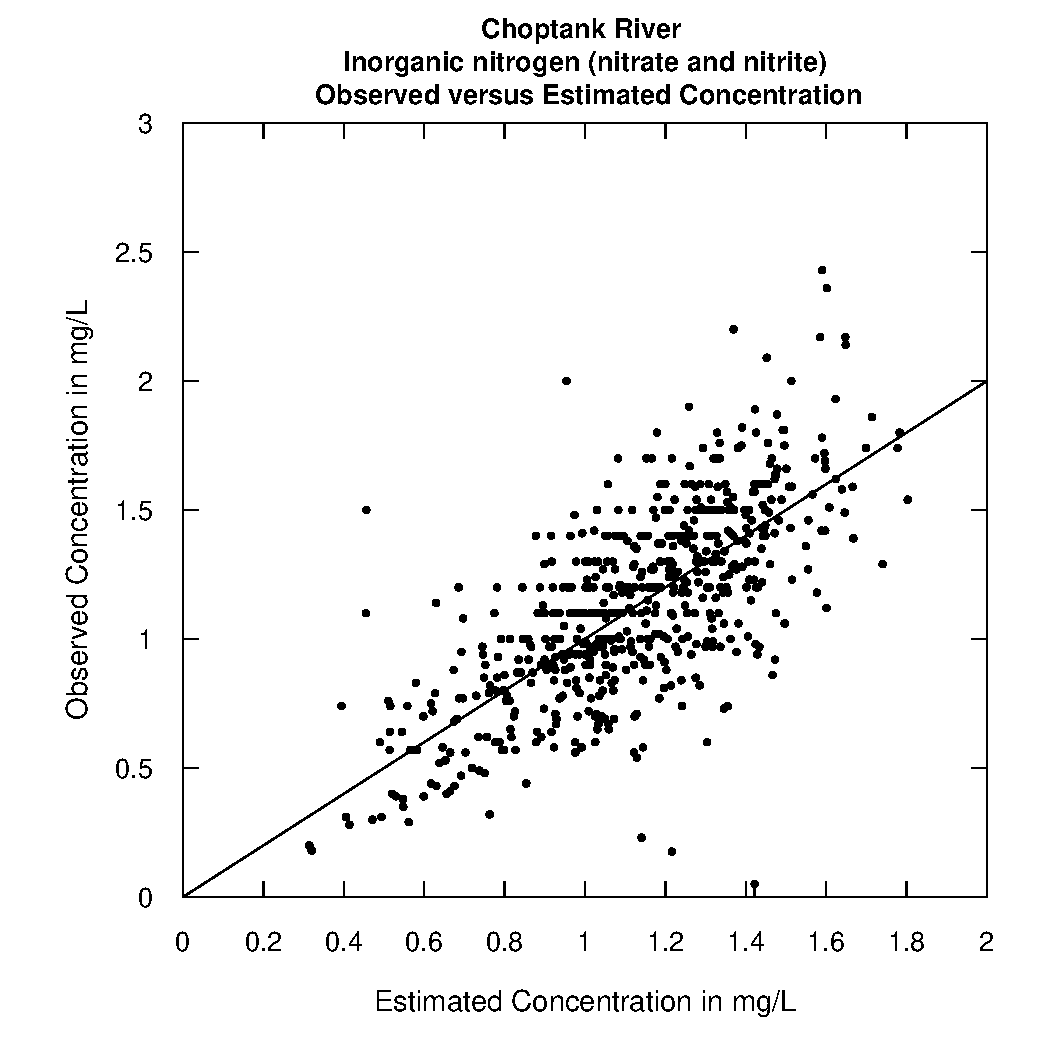
\includegraphics[width=.5\linewidth,height=.5\linewidth]{figure/plotFluxPred1} }
\subfloat[plotLogConcPred()\label{fig:plotFluxPred2}]{
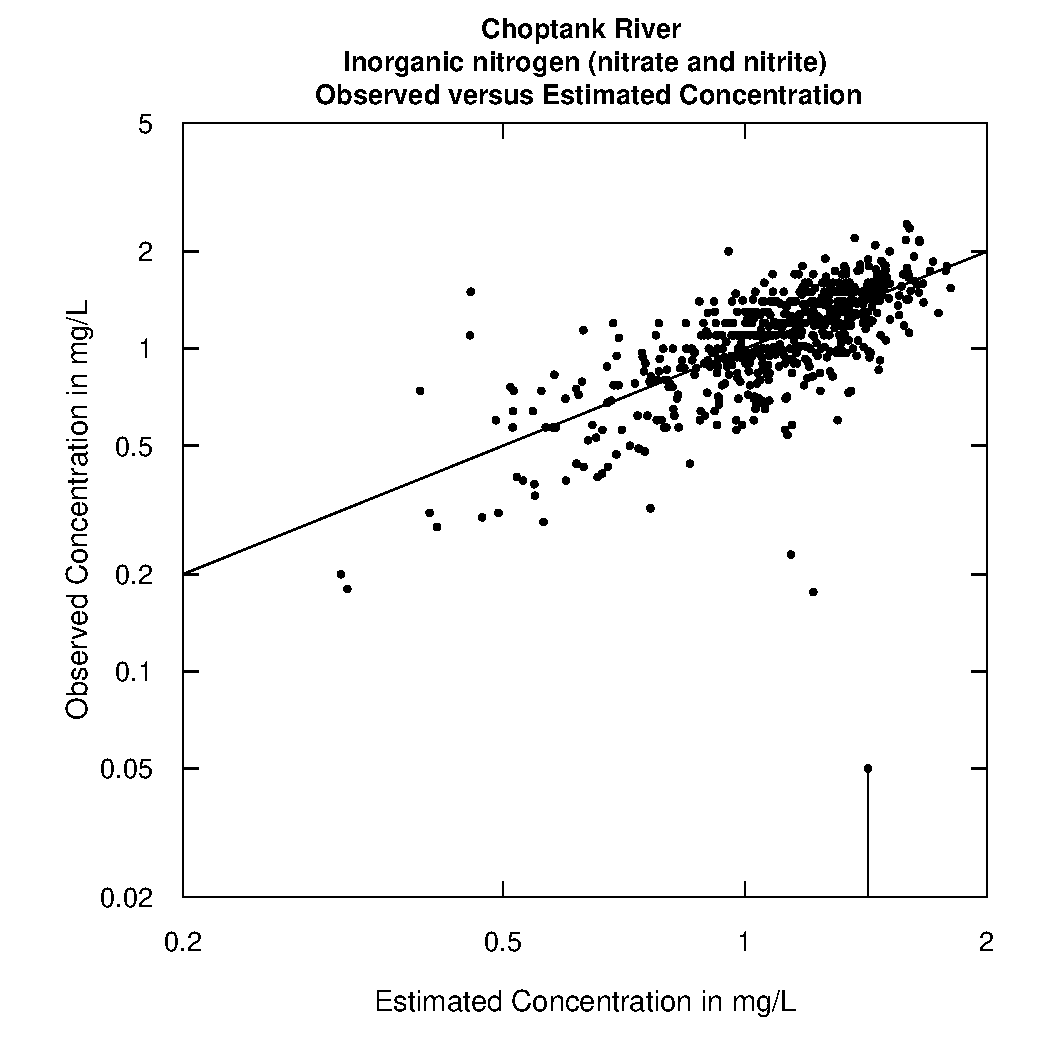
\includegraphics[width=.5\linewidth,height=.5\linewidth]{figure/plotFluxPred2} }\caption[Concentration predictions]{Concentration predictions\label{fig:plotFluxPred}}
\end{figure}


\end{knitrout}


Figure \ref{fig:plotLogFluxPred}:
\begin{knitrout}
\definecolor{shadecolor}{rgb}{0.969, 0.969, 0.969}\color{fgcolor}\begin{kframe}
\begin{alltt}
\hlfunctioncall{plotFluxPred}()
\hlfunctioncall{plotLogFluxPred}()
\end{alltt}
\end{kframe}\begin{figure}[]
\subfloat[plotFluxPred()\label{fig:plotLogFluxPred1}]{
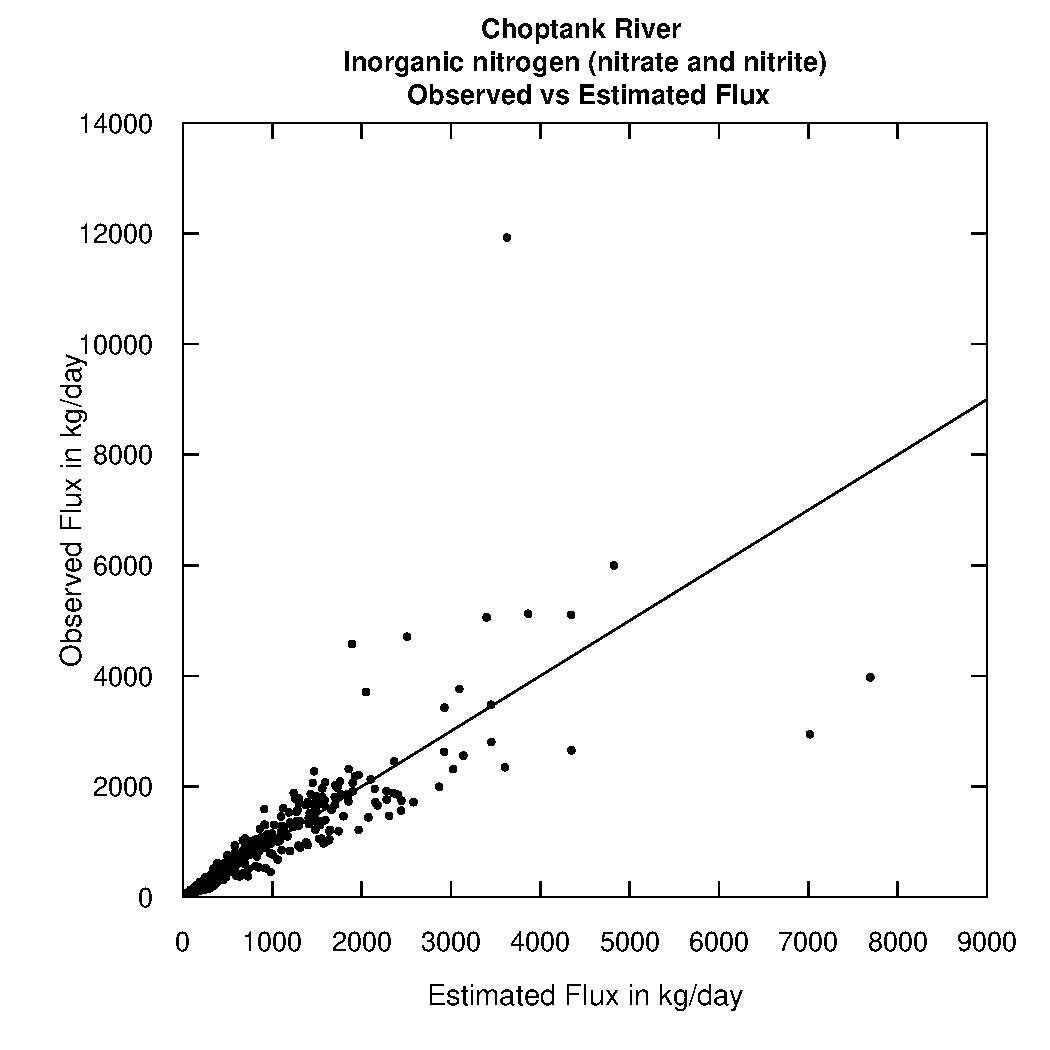
\includegraphics[width=.5\linewidth,height=.5\linewidth]{figure/plotLogFluxPred1} }
\subfloat[plotLogFluxPred()\label{fig:plotLogFluxPred2}]{
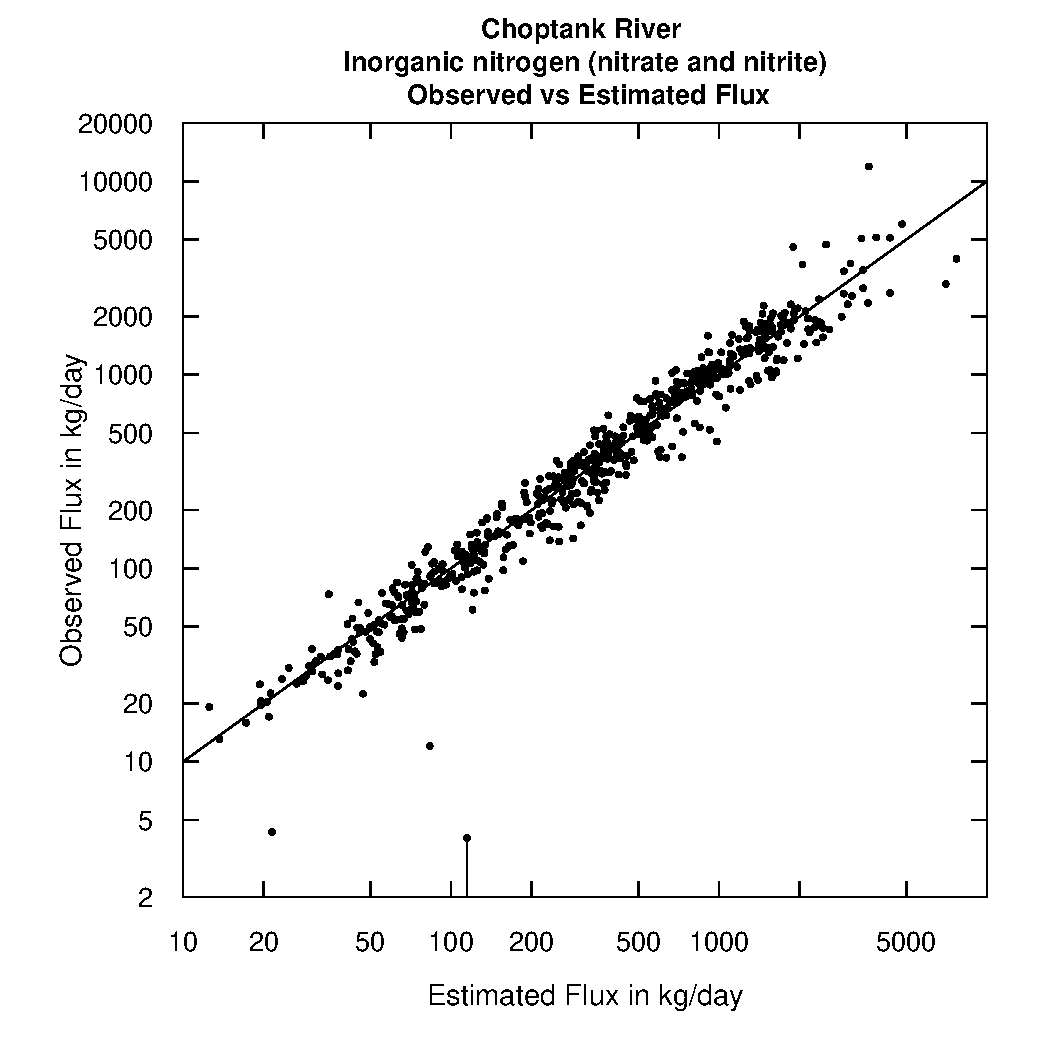
\includegraphics[width=.5\linewidth,height=.5\linewidth]{figure/plotLogFluxPred2} }\caption[Flux predictions]{Flux predictions\label{fig:plotLogFluxPred}}
\end{figure}


\end{knitrout}


Figure \ref{fig:plotResidQ}:
\begin{knitrout}
\definecolor{shadecolor}{rgb}{0.969, 0.969, 0.969}\color{fgcolor}\begin{kframe}
\begin{alltt}
\hlfunctioncall{plotResidPred}()
\hlfunctioncall{plotResidQ}(qUnit=1)
\end{alltt}
\end{kframe}\begin{figure}[]
\subfloat[plotResidPred()\label{fig:plotResidQ1}]{
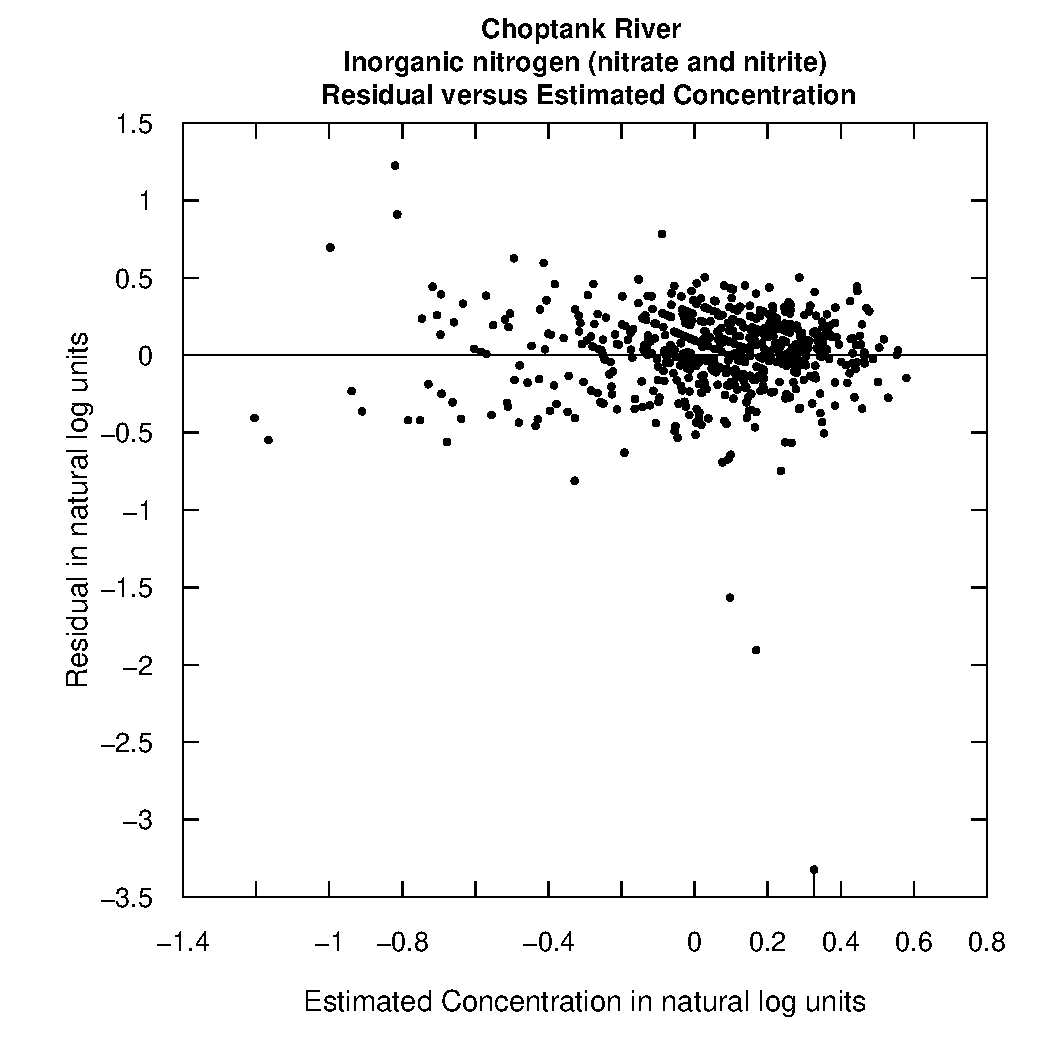
\includegraphics[width=.5\linewidth,height=.5\linewidth]{figure/plotResidQ1} }
\subfloat[plotResidQ(qUnit=1)\label{fig:plotResidQ2}]{
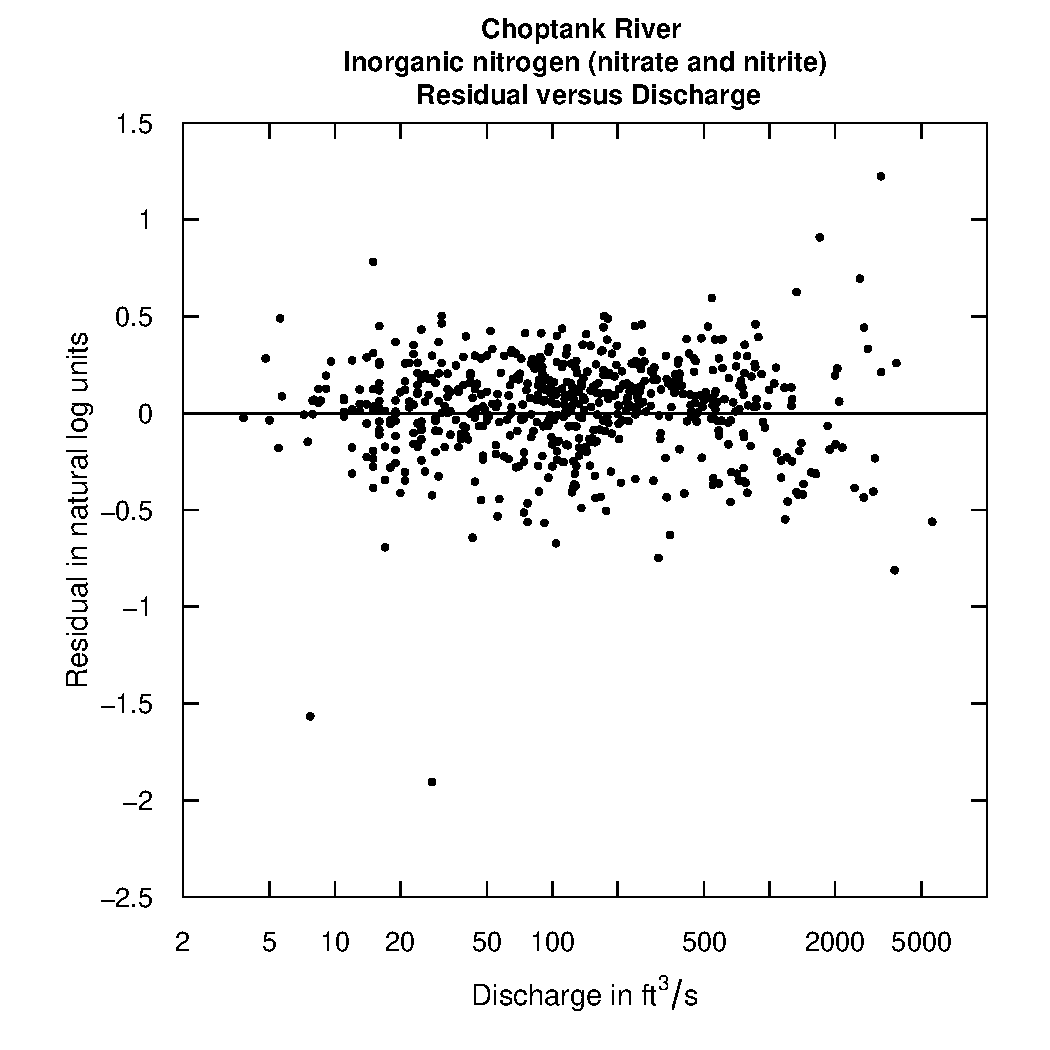
\includegraphics[width=.5\linewidth,height=.5\linewidth]{figure/plotResidQ2} }\caption[Residuals]{Residuals\label{fig:plotResidQ}}
\end{figure}


\end{knitrout}


Figure \ref{fig:boxResidMonth}:
\begin{knitrout}
\definecolor{shadecolor}{rgb}{0.969, 0.969, 0.969}\color{fgcolor}\begin{kframe}
\begin{alltt}
\hlfunctioncall{plotResidTime}()
\hlfunctioncall{boxResidMonth}()
\end{alltt}
\end{kframe}\begin{figure}[]
\subfloat[plotResidTime()\label{fig:boxResidMonth1}]{
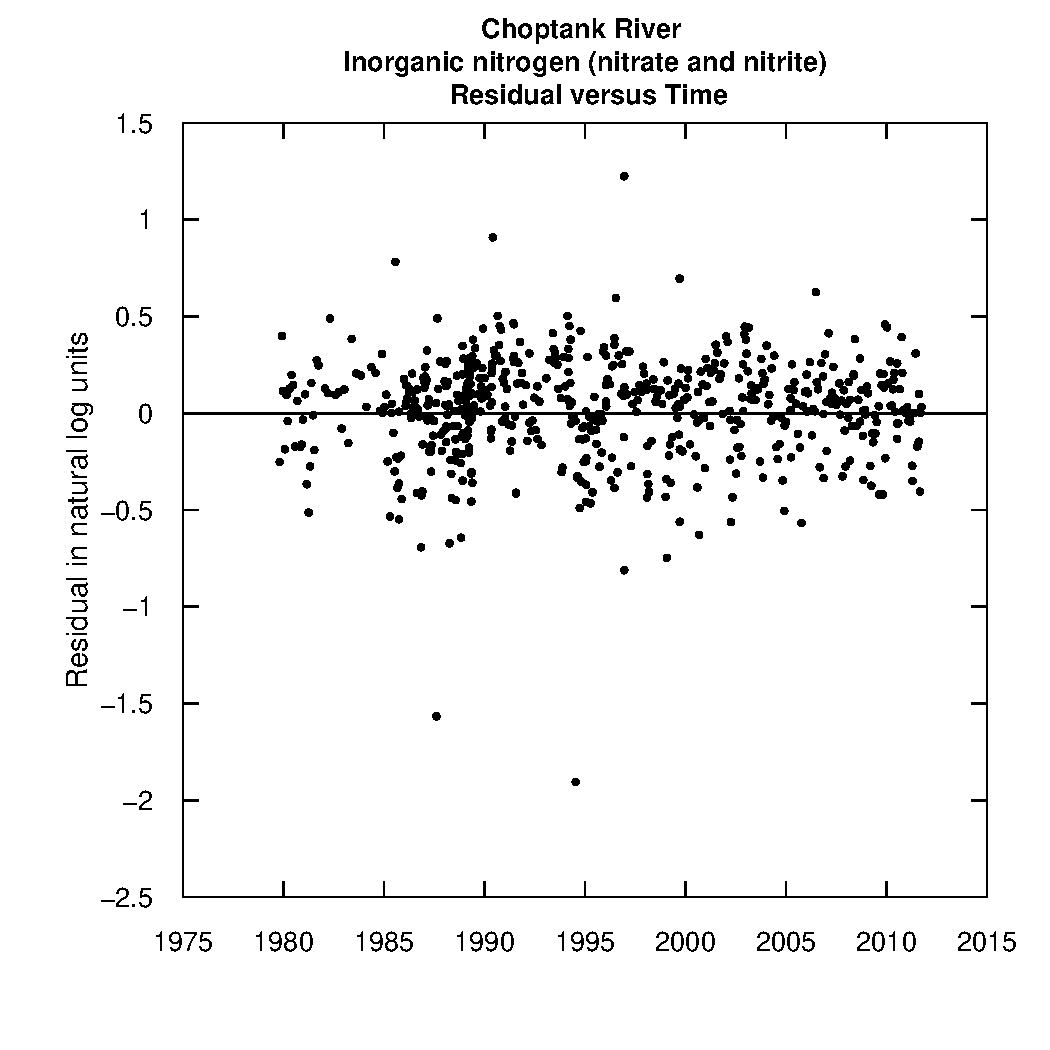
\includegraphics[width=.5\linewidth,height=.5\linewidth]{figure/boxResidMonth1} }
\subfloat[boxResidMonth()\label{fig:boxResidMonth2}]{
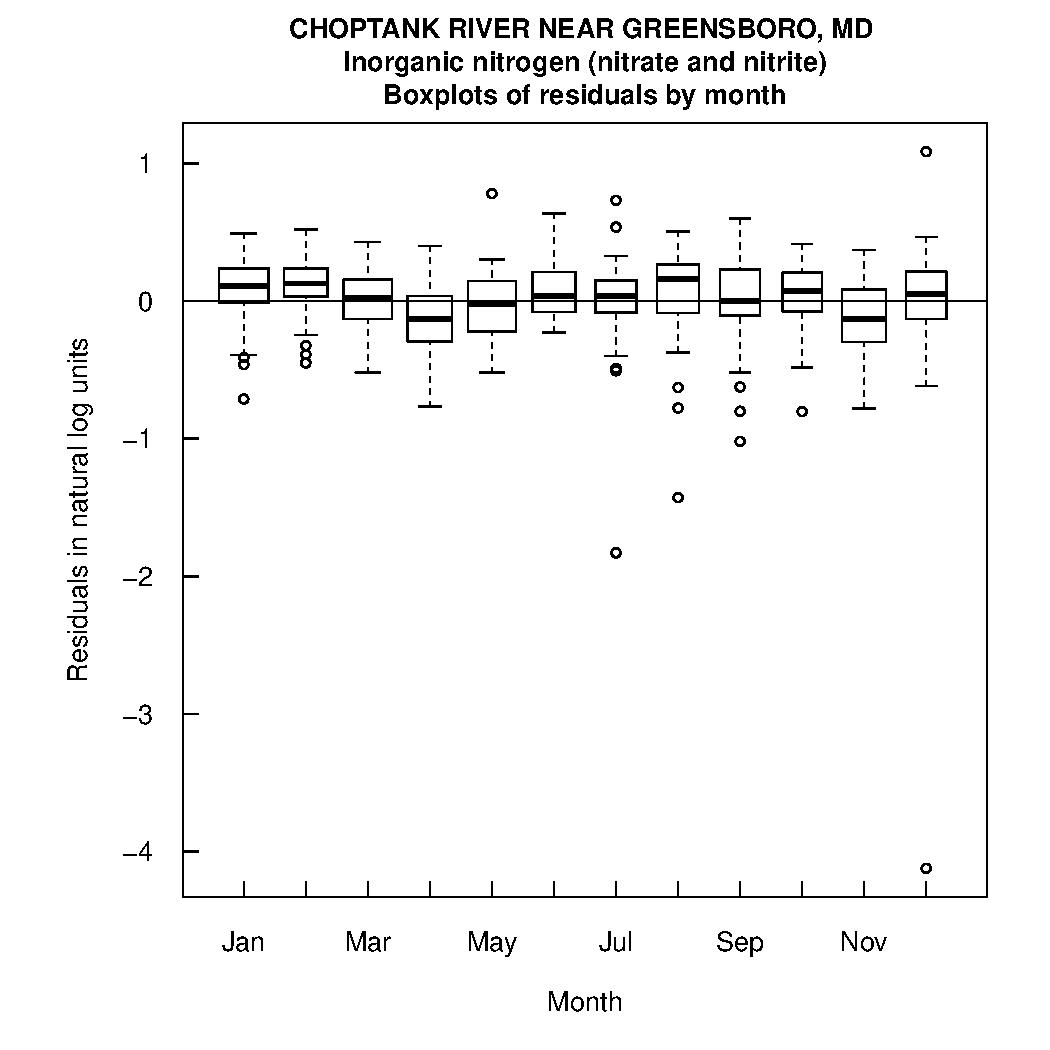
\includegraphics[width=.5\linewidth,height=.5\linewidth]{figure/boxResidMonth2} }\caption[Residuals with respect to time]{Residuals with respect to time\label{fig:boxResidMonth}}
\end{figure}


\end{knitrout}


Figure \ref{fig:boxConcThree}:
\begin{knitrout}
\definecolor{shadecolor}{rgb}{0.969, 0.969, 0.969}\color{fgcolor}\begin{kframe}
\begin{alltt}
\hlfunctioncall{boxConcThree}()
\end{alltt}
\end{kframe}\begin{figure}[]

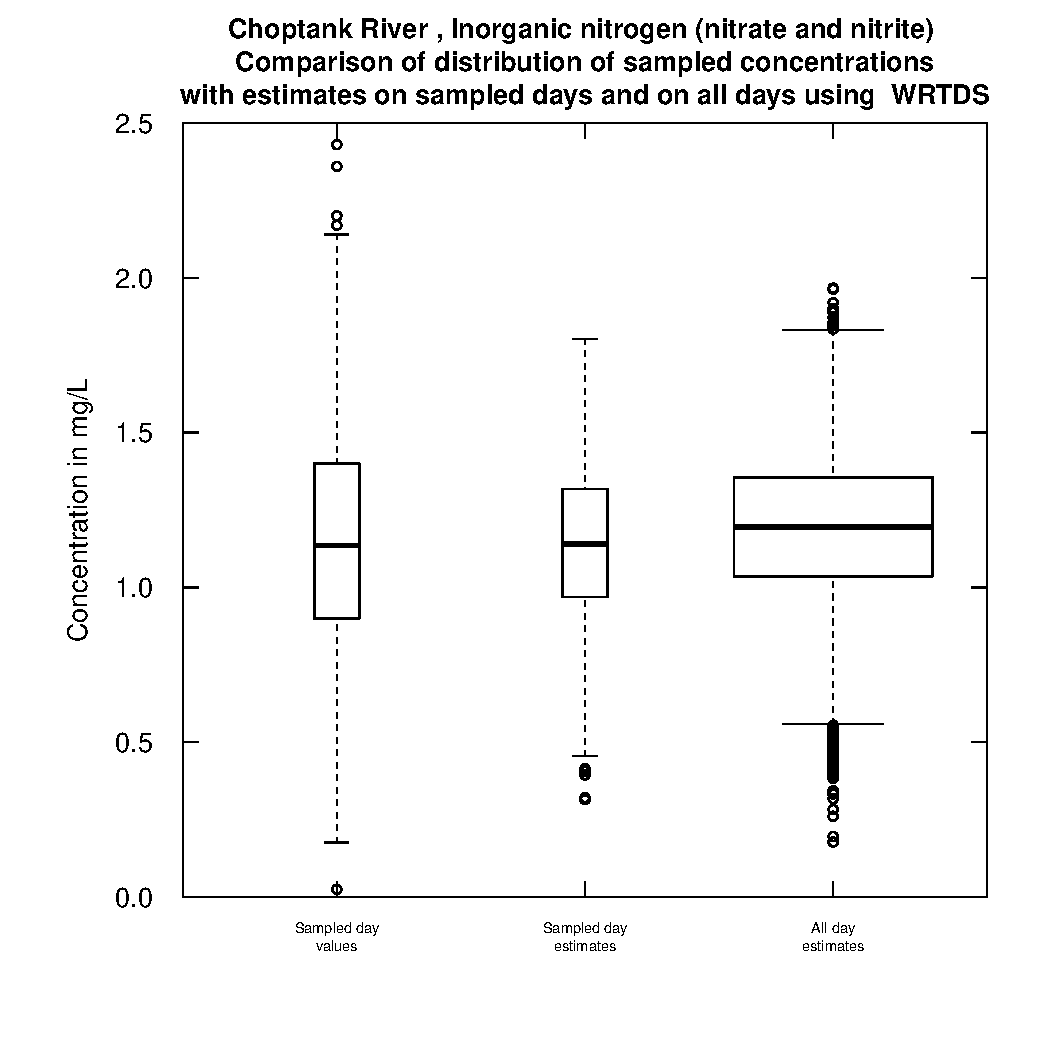
\includegraphics[width=.5\linewidth,height=.5\linewidth]{figure/boxConcThree} \caption[Default boxConcThree()]{Default boxConcThree()\label{fig:boxConcThree}}
\end{figure}


\end{knitrout}


Figure \ref{fig:plotFluxHist}:
\begin{knitrout}
\definecolor{shadecolor}{rgb}{0.969, 0.969, 0.969}\color{fgcolor}\begin{kframe}
\begin{alltt}
\hlfunctioncall{plotConcHist}()
\hlfunctioncall{plotFluxHist}()
\end{alltt}
\end{kframe}\begin{figure}[]
\subfloat[plotConcHist()\label{fig:plotFluxHist1}]{
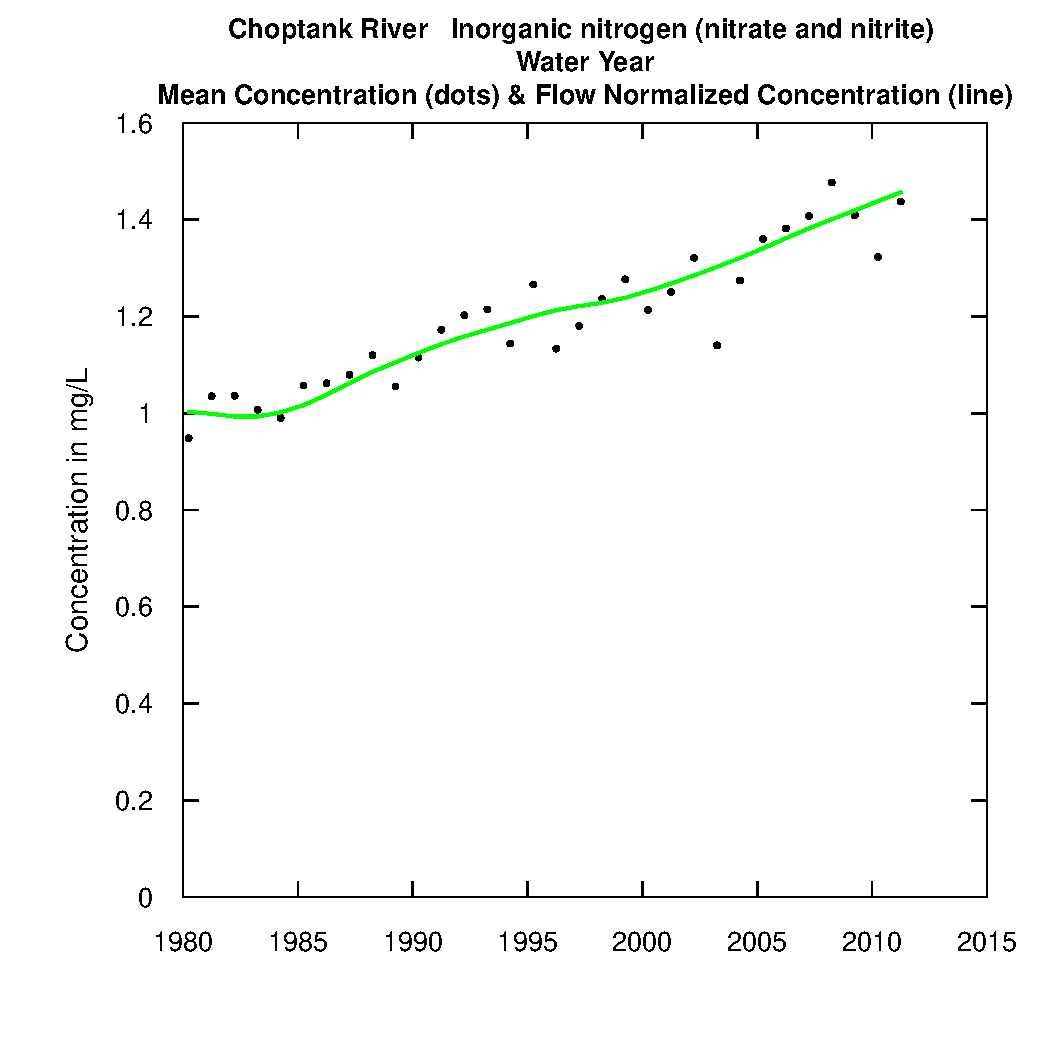
\includegraphics[width=.5\linewidth,height=.5\linewidth]{figure/plotFluxHist1} }
\subfloat[plotFluxHist()\label{fig:plotFluxHist2}]{
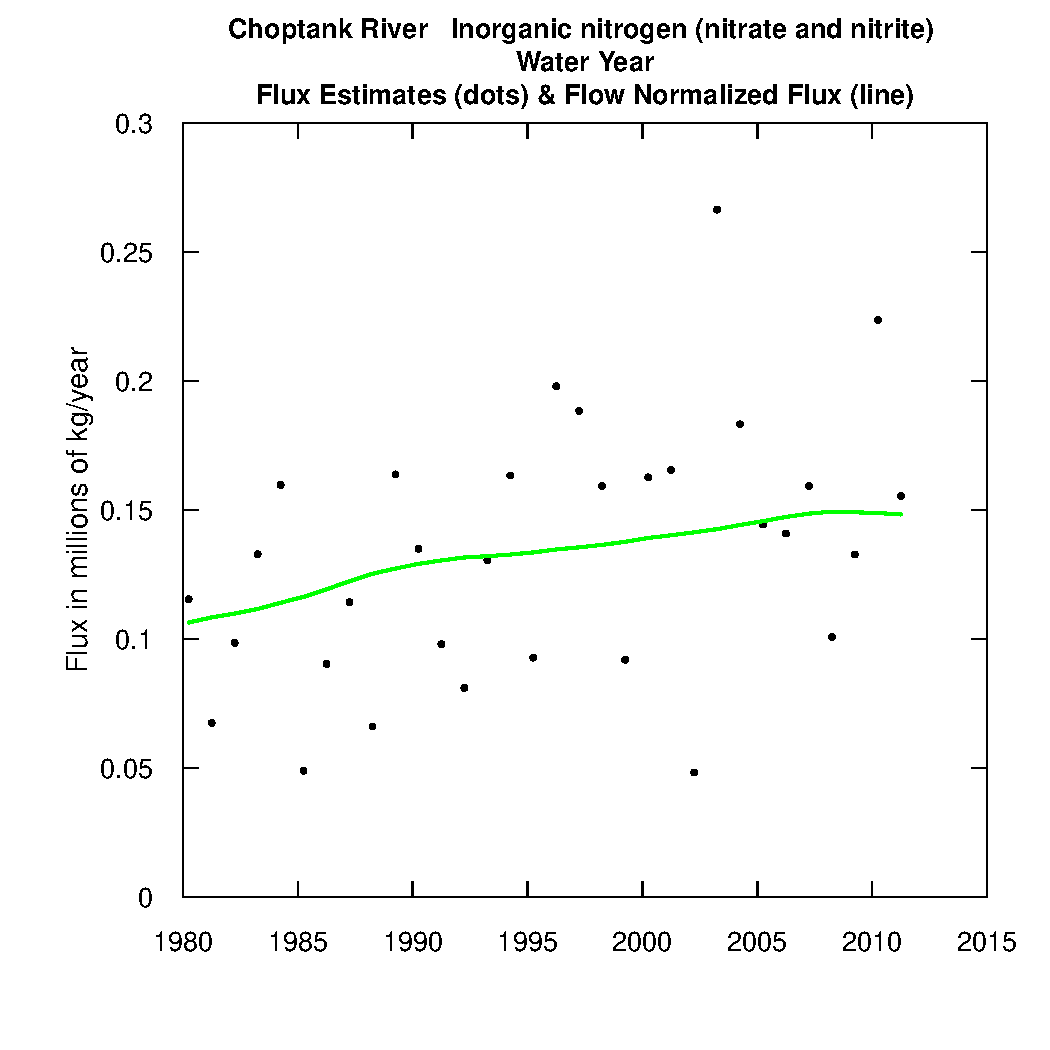
\includegraphics[width=.5\linewidth,height=.5\linewidth]{figure/plotFluxHist2} }\caption[Concentration and flux history]{Concentration and flux history\label{fig:plotFluxHist}}
\end{figure}


\end{knitrout}


Figure \ref{fig:plotLogConcQSmooth}:
\begin{knitrout}
\definecolor{shadecolor}{rgb}{0.969, 0.969, 0.969}\color{fgcolor}\begin{kframe}
\begin{alltt}
qBottom<-1
qTop<-5000
date1 <- \hlstring{"2000-09-01"}
date2 <- \hlstring{"2005-09-01"}
date3 <- \hlstring{"2009-09-01"}
\hlfunctioncall{plotConcQSmooth}(date1, date2, date3, qBottom, qTop, 
                   concMax=1.5,qUnit=1)
\hlfunctioncall{plotLogConcQSmooth}(date1, date2, date3, qBottom, qTop,
                   concMax=1.5, concMin=0.1,qUnit=1)
\end{alltt}
\end{kframe}\begin{figure}[]
\subfloat[plotConcQSmooth\label{fig:plotLogConcQSmooth1}]{
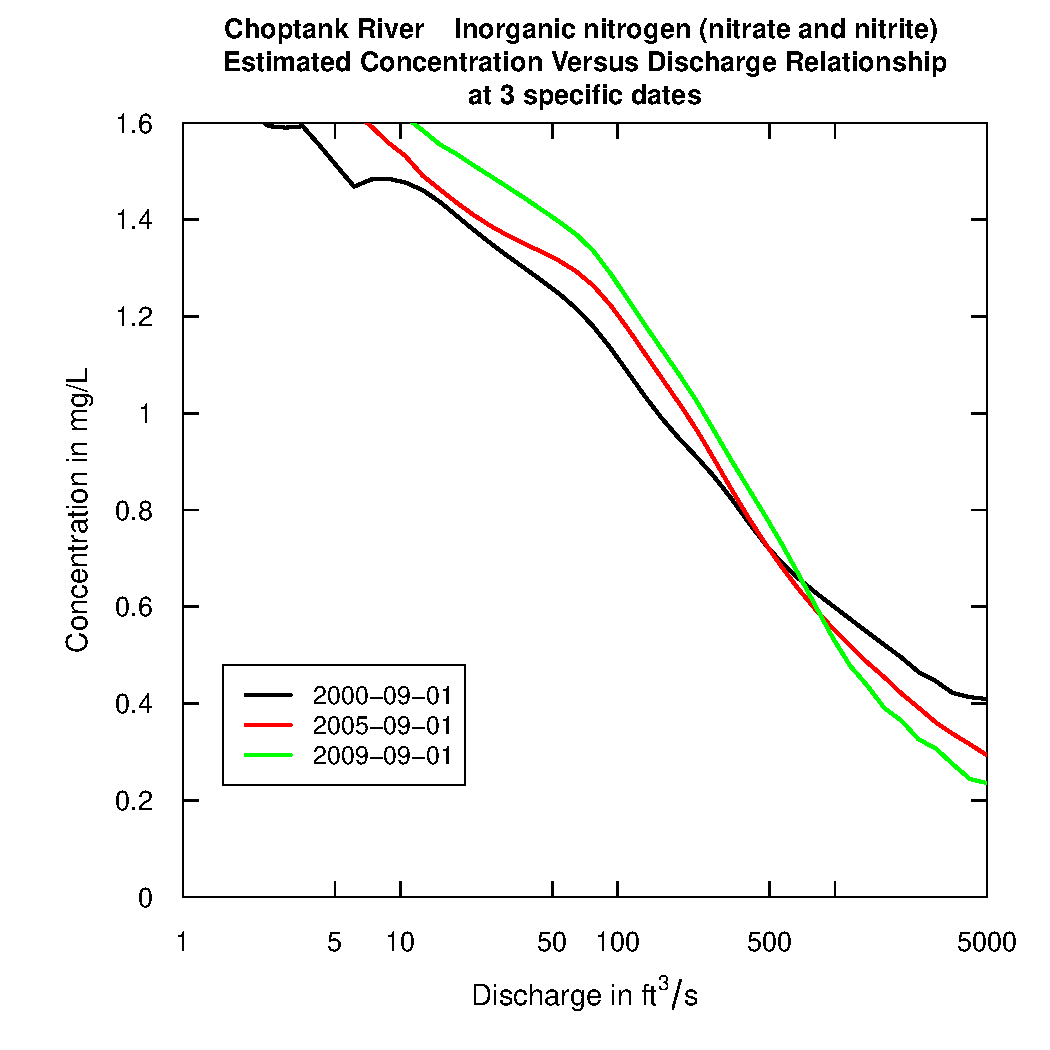
\includegraphics[width=.5\linewidth,height=.5\linewidth]{figure/plotLogConcQSmooth1} }
\subfloat[plotLogConcQSmooth\label{fig:plotLogConcQSmooth2}]{
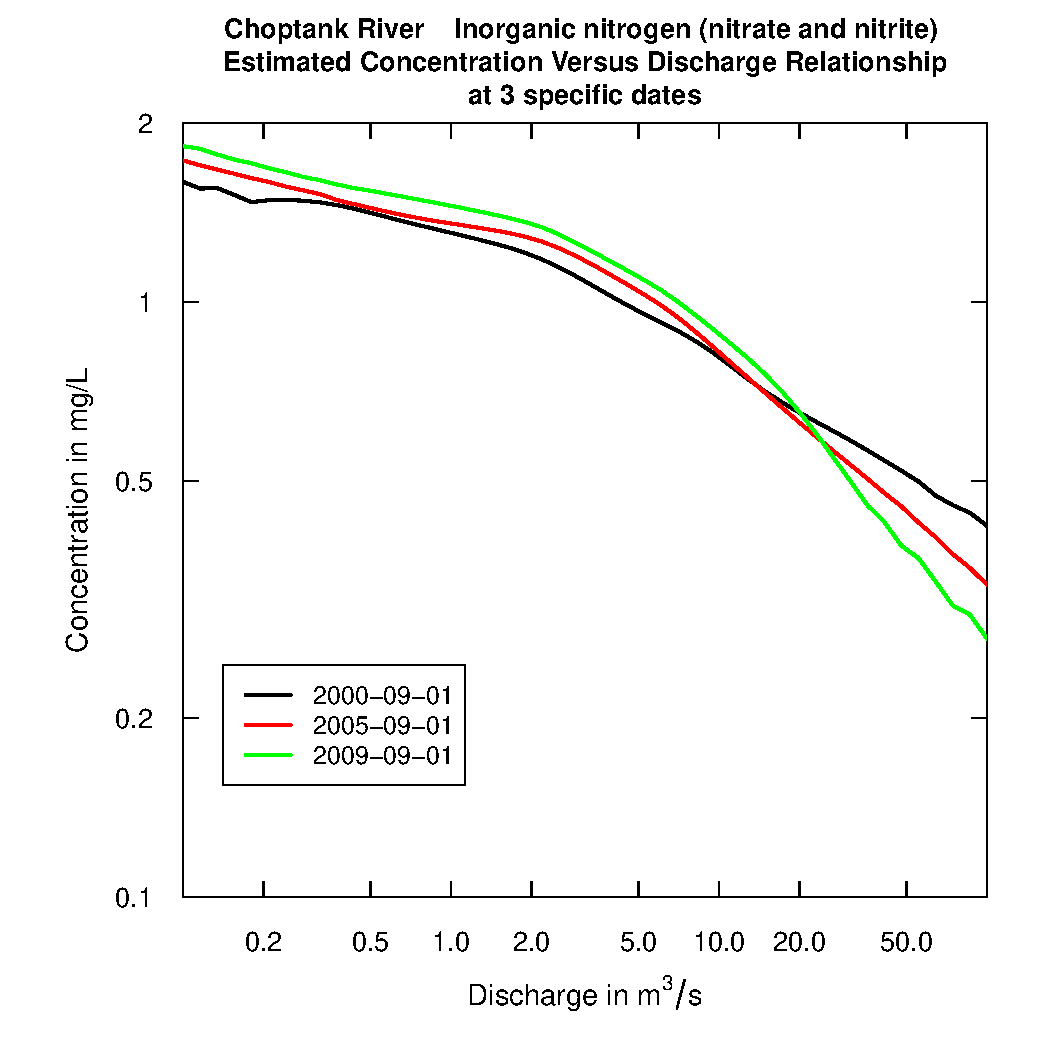
\includegraphics[width=.5\linewidth,height=.5\linewidth]{figure/plotLogConcQSmooth2} }\caption[Concentration vs]{Concentration vs. discharge\label{fig:plotLogConcQSmooth}}
\end{figure}


\end{knitrout}


Figure \ref{fig:plotConcTimeSmooth}:
\begin{knitrout}
\definecolor{shadecolor}{rgb}{0.969, 0.969, 0.969}\color{fgcolor}\begin{kframe}
\begin{alltt}
q1 <- 10
q2 <- 25
q3 <- 75
centerDate <- \hlstring{"07-01"}
\hlfunctioncall{plotConcTimeSmooth}(q1, q2, q3, centerDate, 2000, 2010)
\end{alltt}
\end{kframe}\begin{figure}[]

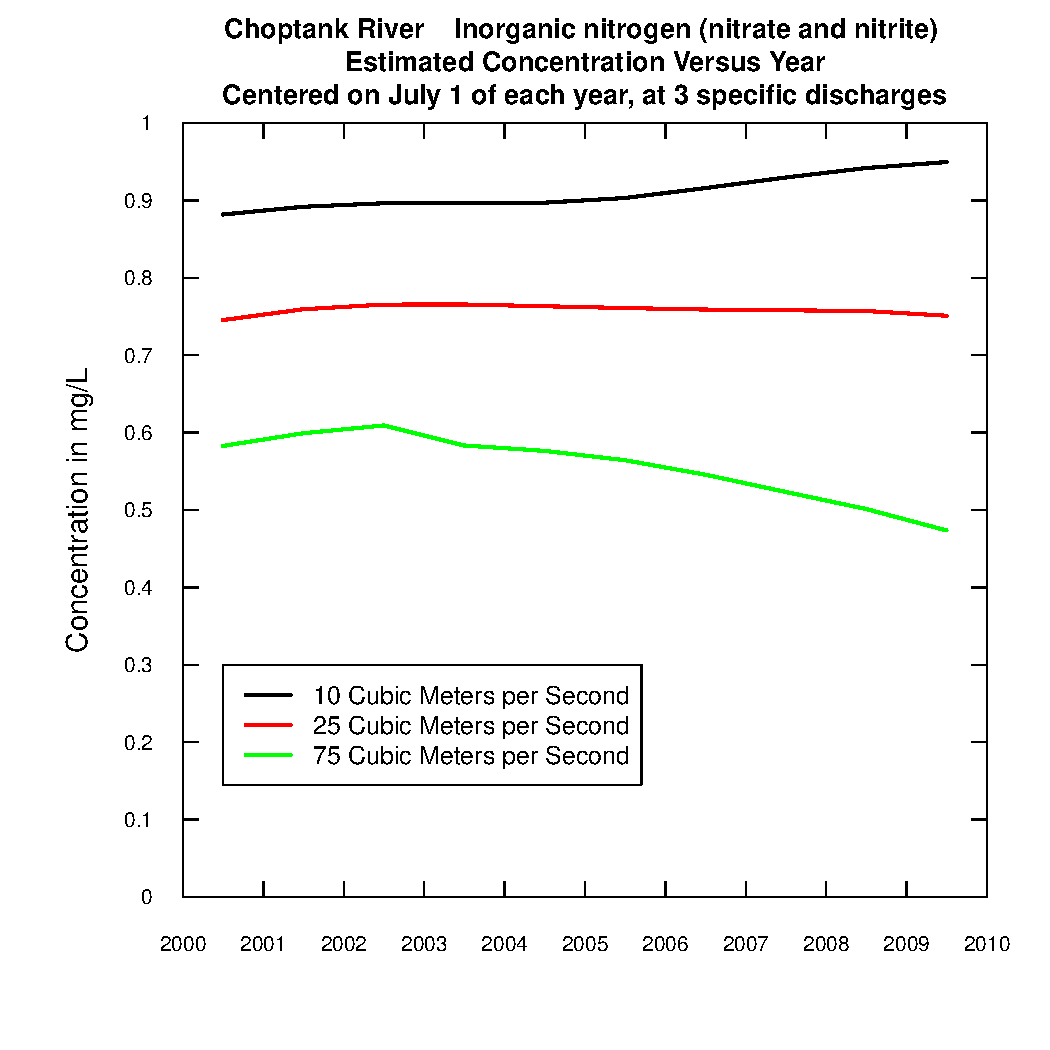
\includegraphics[width=.5\linewidth,height=.5\linewidth]{figure/plotConcTimeSmooth} \caption[plotConcTimeSmooth]{plotConcTimeSmooth\label{fig:plotConcTimeSmooth}}
\end{figure}


\end{knitrout}


Figure \ref{fig:fluxBiasMulti}:
\begin{knitrout}
\definecolor{shadecolor}{rgb}{0.969, 0.969, 0.969}\color{fgcolor}\begin{kframe}
\begin{alltt}
\hlfunctioncall{fluxBiasMulti}(qUnit=1)
\end{alltt}
\end{kframe}\begin{figure}[]

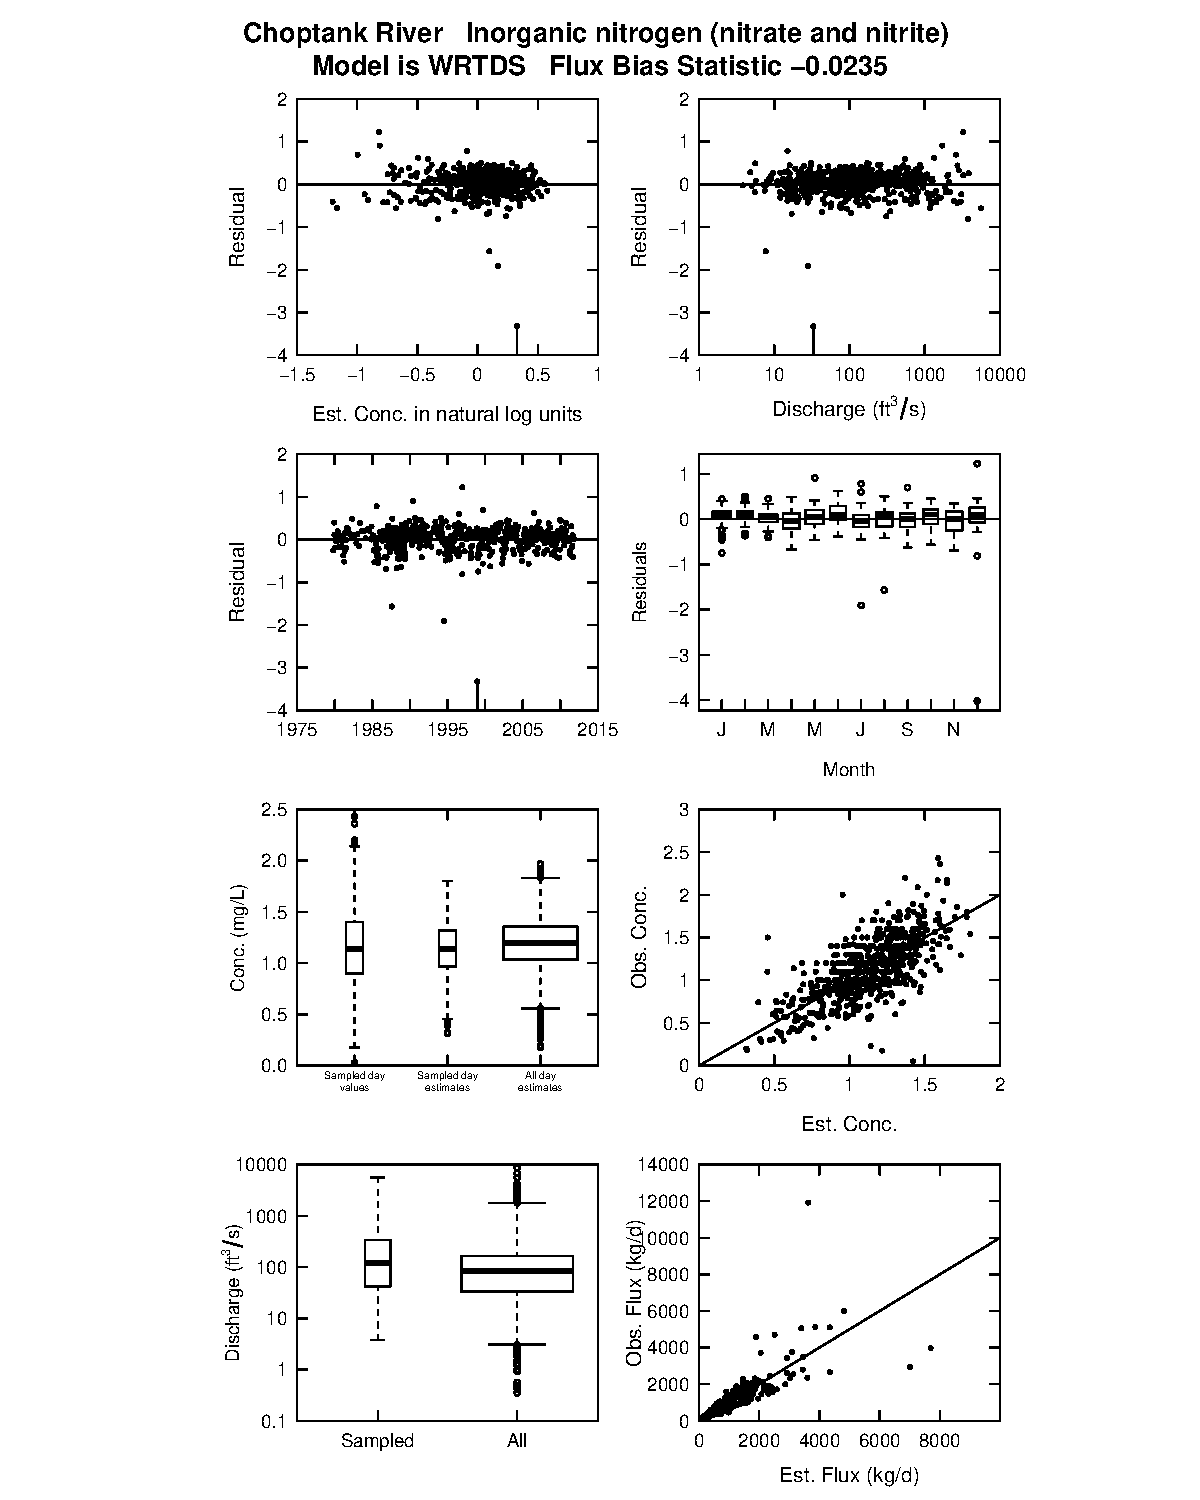
\includegraphics[width=1\linewidth,height=1\linewidth]{figure/fluxBiasMulti} \caption[fluxBiasMulti(qUnit=1)]{fluxBiasMulti(qUnit=1)\label{fig:fluxBiasMulti}}
\end{figure}


\end{knitrout}


Figure \ref{fig:fluxBiasMultiAlt}:
\begin{knitrout}
\definecolor{shadecolor}{rgb}{0.969, 0.969, 0.969}\color{fgcolor}\begin{kframe}
\begin{alltt}
\hlfunctioncall{fluxBiasMultiAlt}(qUnit=1)
\end{alltt}
\end{kframe}\begin{figure}[]

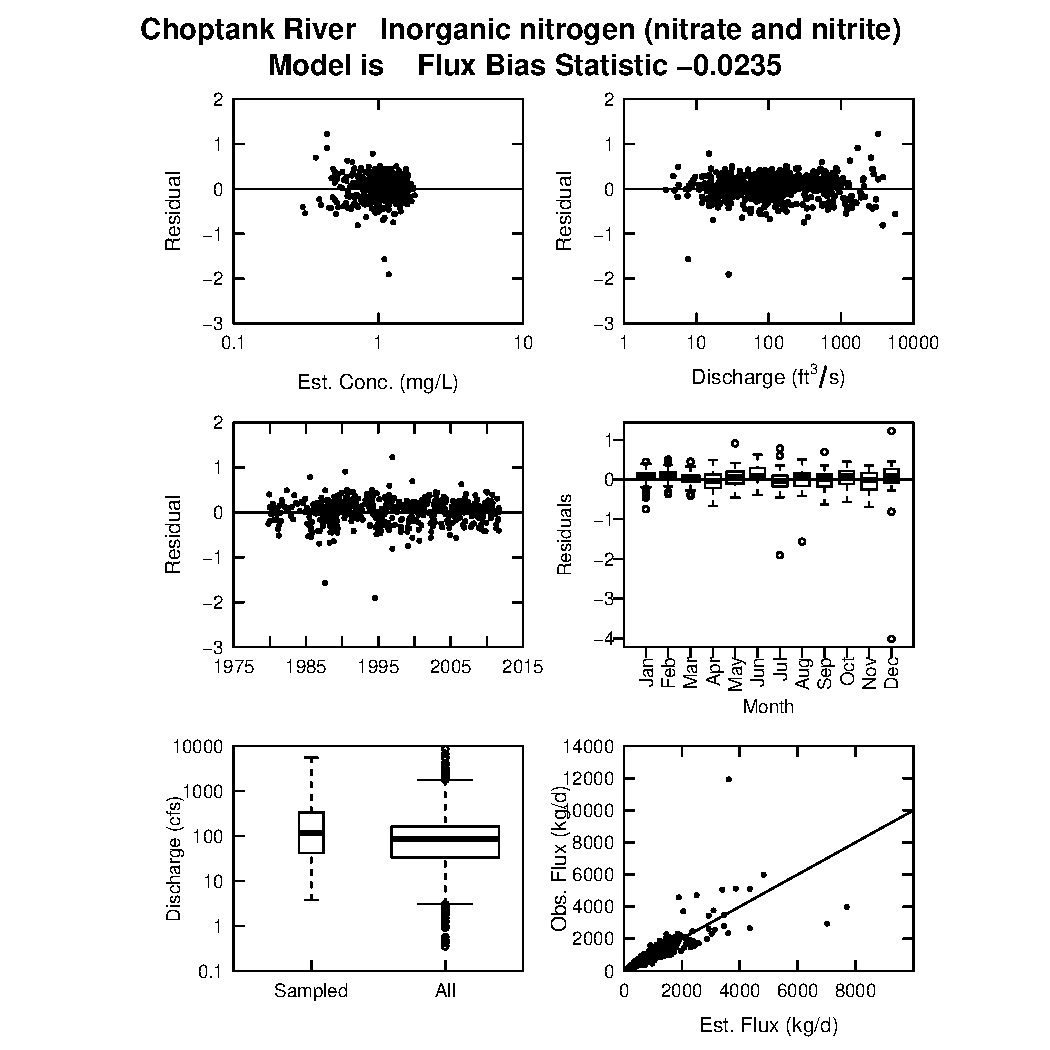
\includegraphics[width=1\linewidth,height=1\linewidth]{figure/fluxBiasMultiAlt} \caption[fluxBiasMultiAlt(qUnit=1)]{fluxBiasMultiAlt(qUnit=1)\label{fig:fluxBiasMultiAlt}}
\end{figure}


\end{knitrout}


Figure \ref{fig:fluxBiasEight}:
\begin{knitrout}
\definecolor{shadecolor}{rgb}{0.969, 0.969, 0.969}\color{fgcolor}\begin{kframe}
\begin{alltt}
\hlfunctioncall{fluxBiasEight}(qUnit=1)
\end{alltt}
\end{kframe}\begin{figure}[]

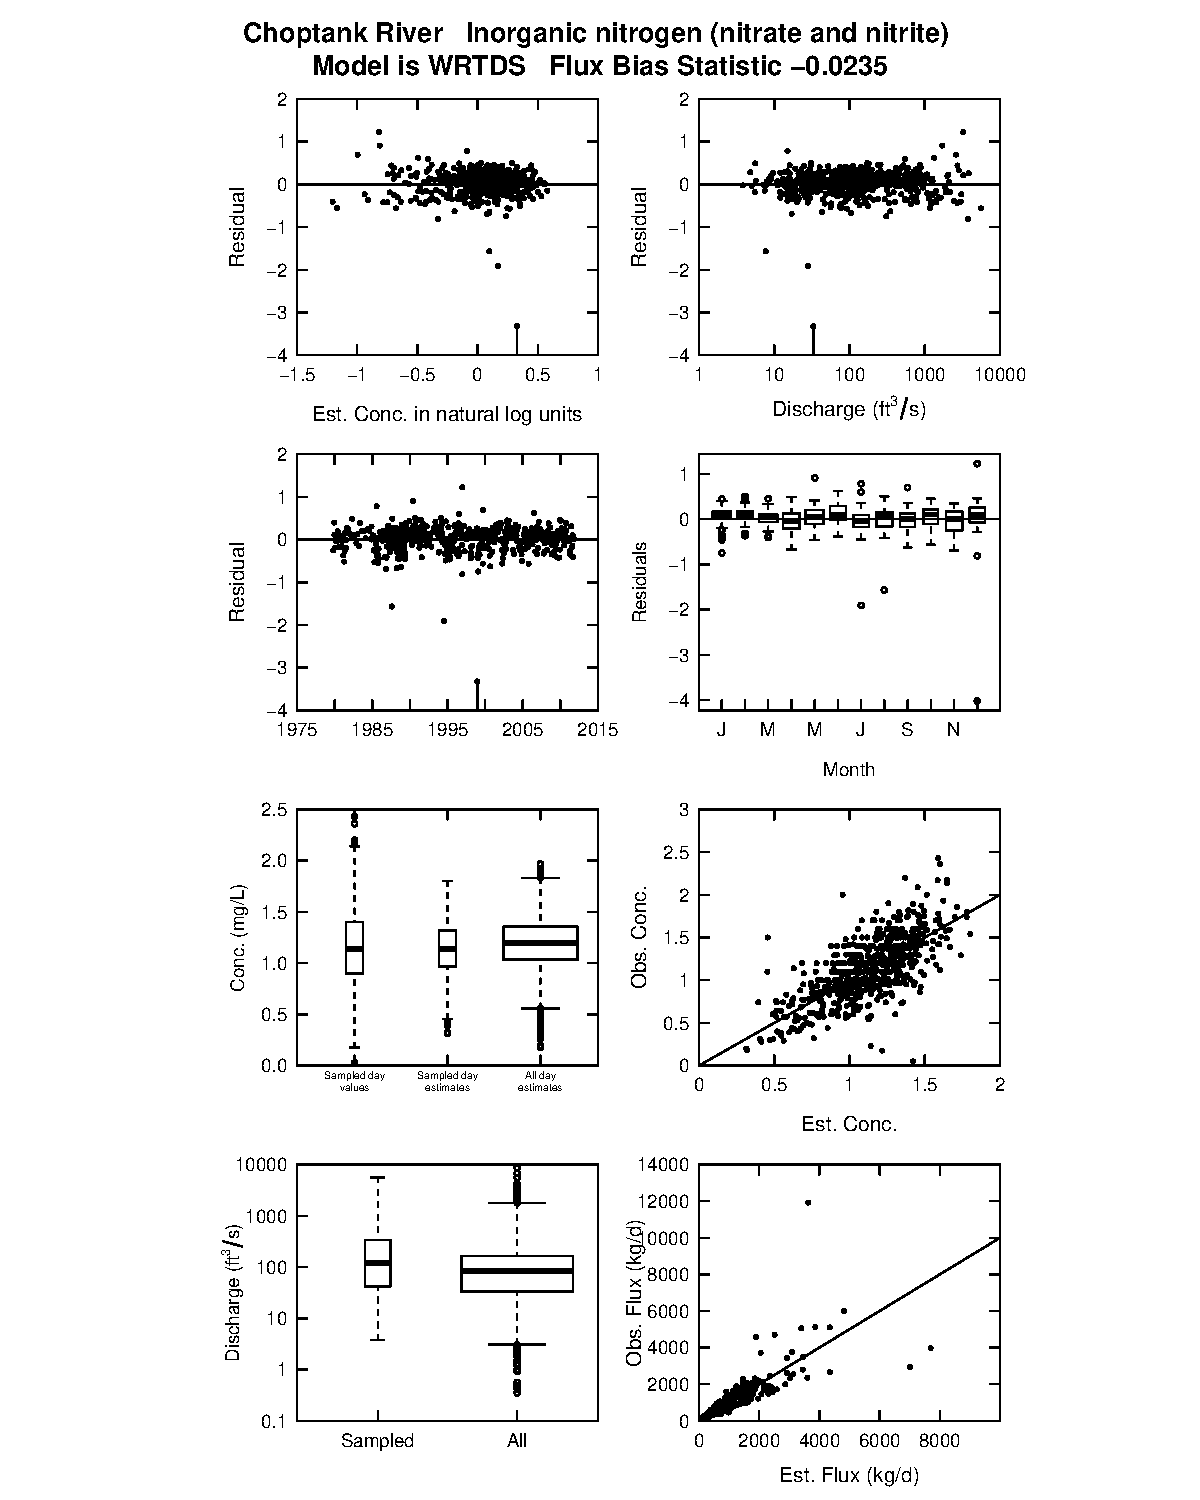
\includegraphics[width=\maxwidth]{figure/fluxBiasEight} \caption[fluxBiasEight(qUnit=1)]{fluxBiasEight(qUnit=1)\label{fig:fluxBiasEight}}
\end{figure}


\end{knitrout}


Figure \ref{fig:plotContours}:
\begin{knitrout}
\definecolor{shadecolor}{rgb}{0.969, 0.969, 0.969}\color{fgcolor}\begin{kframe}
\begin{alltt}
clevel<-\hlfunctioncall{seq}(0,2,0.5)
\hlfunctioncall{plotContours}(yearStart,yearEnd,qBottom,qTop, 
             contourLevels = clevel,qUnit=1)
\end{alltt}
\end{kframe}\begin{figure}[]

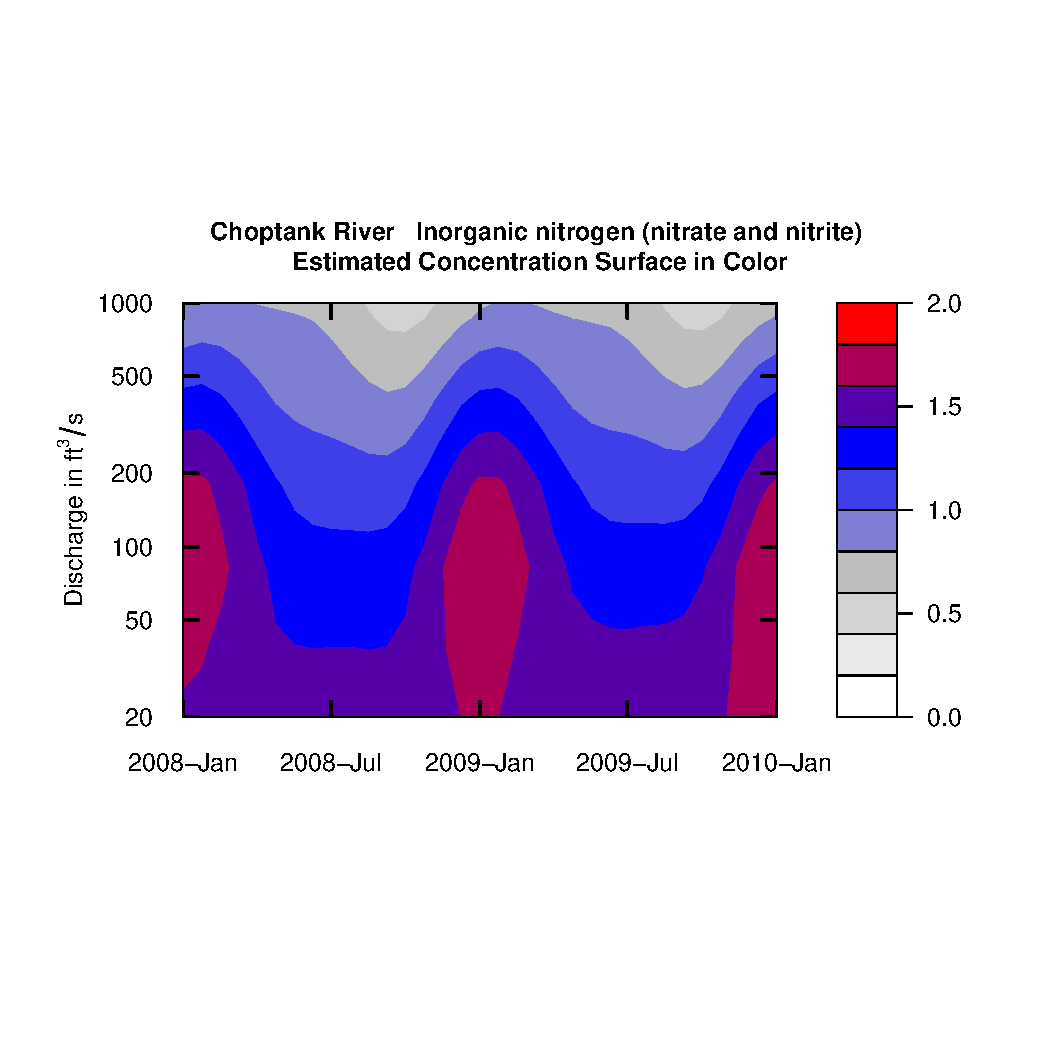
\includegraphics[width=1\linewidth,height=1\linewidth]{figure/plotContours} \caption[plotContours(2008,2010,1,5000,clevel,qUnit=1)]{plotContours(2008,2010,1,5000,clevel,qUnit=1)\label{fig:plotContours}}
\end{figure}


\end{knitrout}


Figure \ref{fig:plotDiffContours}:
\begin{knitrout}
\definecolor{shadecolor}{rgb}{0.969, 0.969, 0.969}\color{fgcolor}\begin{kframe}
\begin{alltt}
maxDiff<-2
\hlfunctioncall{plotDiffContours}(year0=2000,yearEnd,
                 qBottom,qTop,maxDiff,qUnit=1)
\end{alltt}
\end{kframe}\begin{figure}[]

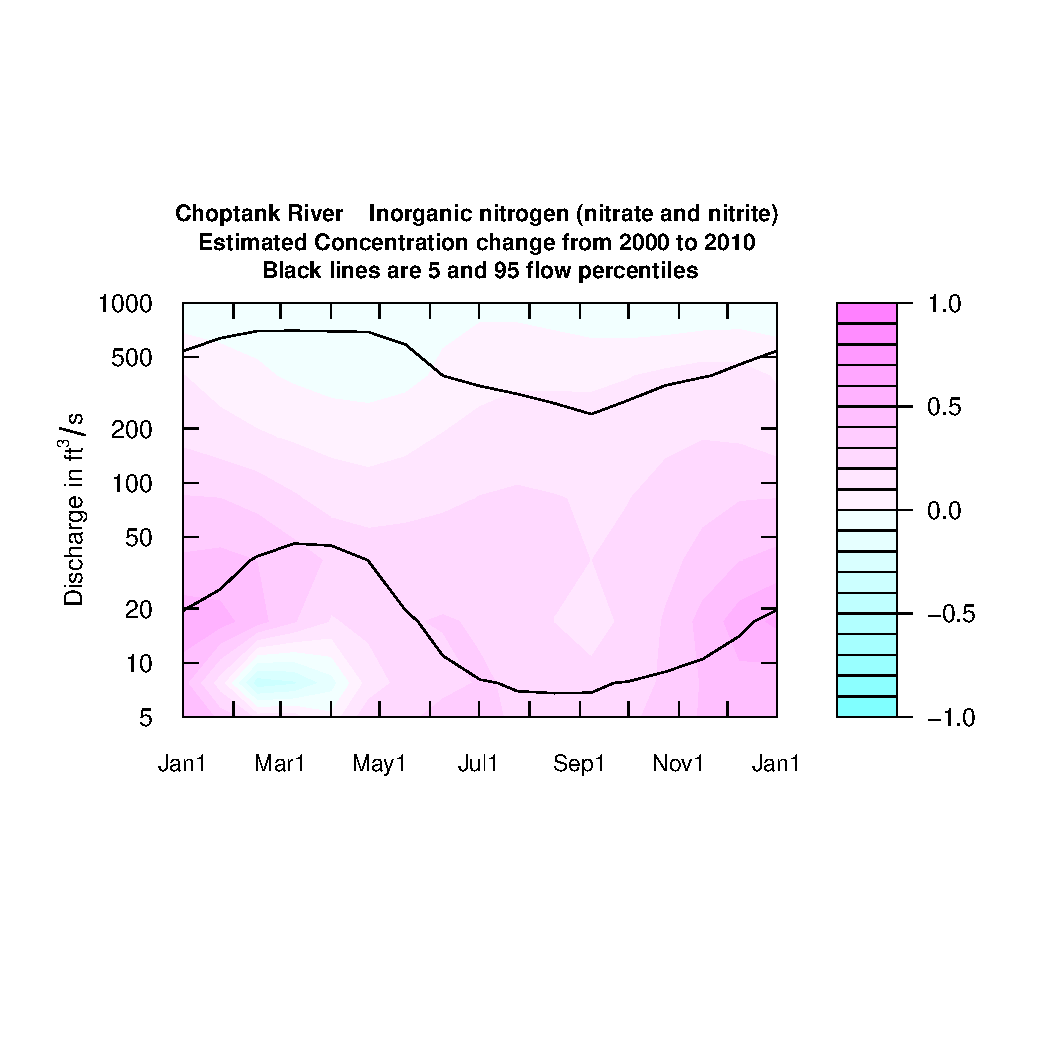
\includegraphics[width=1\linewidth,height=1\linewidth]{figure/plotDiffContours} \caption[plotDiffContours(year0=2000,yearEnd=2010,qBottom=1,qTop=5000,maxDiff=2)]{plotDiffContours(year0=2000,yearEnd=2010,qBottom=1,qTop=5000,maxDiff=2)\label{fig:plotDiffContours}}
\end{figure}


\end{knitrout}



To specify contourLevels the seq function in R should be used.  In general it would look like this: contourLevels = seq(from,to,by).  For example, if we want contours to run from 0 to 5 in steps of 0.2 we would say:  

\begin{knitrout}
\definecolor{shadecolor}{rgb}{0.969, 0.969, 0.969}\color{fgcolor}\begin{kframe}
\begin{alltt}
contourLevels = \hlfunctioncall{seq}(0,5,0.2)
\end{alltt}
\end{kframe}
\end{knitrout}



\FloatBarrier
%------------------------------------------------------------ 
\subsection{Table Options}
\label{sec:wrtdsTable}
%------------------------------------------------------------ 
Sometimes easier to consider the results in table formats rather than graphically. The function tableResults produces a simple text table that contains the annual values for the results.  Each row of the output represents a year and it prints: year, average discharge, average concentration, flow normalized concentration, average flux, and flow normalized flux.  

\begin{knitrout}
\definecolor{shadecolor}{rgb}{0.969, 0.969, 0.969}\color{fgcolor}\begin{kframe}
\begin{alltt}
\hlfunctioncall{tableResults}()
\end{alltt}
\begin{verbatim}
## 
##    Choptank River 
##    Inorganic nitrogen (nitrate and nitrite)
##    Water Year 
## 
##    Year   Discharge    Conc    FN_Conc     Flux    FN_Flux
##              cms            mg/L             10^6 kg/yr 
## 
##    1980      4.25     0.949     1.003    0.1154     0.106
##    1981      2.22     1.035     0.999    0.0675     0.108
##    1982      3.05     1.036     0.993    0.0985     0.110
##    1983      4.99     1.007     0.993    0.1329     0.112
##    1984      5.72     0.990     1.002    0.1597     0.114
##    1985      1.52     1.057     1.017    0.0489     0.116
##    1986      2.63     1.062     1.038    0.0903     0.119
##    1987      3.37     1.079     1.062    0.1142     0.122
##    1988      1.87     1.120     1.085    0.0660     0.125
##    1989      5.61     1.055     1.105    0.1638     0.127
##    1990      4.01     1.115     1.125    0.1349     0.129
##    1991      2.75     1.172     1.143    0.0980     0.130
##    1992      2.19     1.203     1.159    0.0810     0.132
##    1993      3.73     1.215     1.173    0.1306     0.132
##    1994      5.48     1.144     1.187    0.1634     0.133
##    1995      2.41     1.266     1.201    0.0928     0.134
##    1996      6.24     1.134     1.213    0.1980     0.135
##    1997      5.83     1.180     1.221    0.1884     0.136
##    1998      4.88     1.236     1.229    0.1593     0.137
##    1999      2.90     1.277     1.238    0.0919     0.138
##    2000      4.72     1.213     1.253    0.1627     0.139
##    2001      4.88     1.251     1.268    0.1655     0.140
##    2002      1.24     1.321     1.285    0.0483     0.141
##    2003      8.64     1.140     1.303    0.2664     0.143
##    2004      5.28     1.274     1.321    0.1832     0.144
##    2005      3.81     1.360     1.341    0.1444     0.146
##    2006      3.59     1.382     1.362    0.1409     0.147
##    2007      4.28     1.408     1.382    0.1593     0.149
##    2008      2.56     1.477     1.401    0.1008     0.149
##    2009      3.68     1.409     1.419    0.1328     0.149
##    2010      7.19     1.323     1.438    0.2236     0.149
##    2011      5.24     1.438     1.457    0.1554     0.148
## NULL
\end{verbatim}
\end{kframe}
\end{knitrout}


\FloatBarrier

Additionally, you can have the tableResults return the results as a dataframe. This can be useful for further R analysis, or creating more visually appealing tables.  For instance, using the xtable package, one can create a \LaTeX table. See Appendix \ref{app:createWordTable} for instructions on converting an R dataframe to a table in Microsoft.

\begin{knitrout}
\definecolor{shadecolor}{rgb}{0.969, 0.969, 0.969}\color{fgcolor}\begin{kframe}
\begin{alltt}
\hlfunctioncall{library}(xtable)
tableOut <- \hlfunctioncall{tableResults}(returnDataFrame = TRUE)
tableOut <- \hlfunctioncall{head}(tableOut)
\hlfunctioncall{xtable}(tableOut, 
    caption=\hlstring{"Table created from tableResults function"},
    label=\hlstring{"table:tableResults"})
\end{alltt}
\end{kframe}
\end{knitrout}


\begin{table}[ht]
\centering
\begin{tabular}{rllllll}
  \hline
 & Year & Discharge [cms] & Conc [mg/L] & FN\_Conc [mg/L] & Flux [10\verb|^|6kg/yr] & FN\_Flux [10\verb|^|6kg/yr] \\ 
  \hline
1 &    1980 &      4.25 &     0.949 &     1.003 &    0.1154 &     0.106 \\ 
  2 &    1981 &      2.22 &     1.035 &     0.999 &    0.0675 &     0.108 \\ 
  3 &    1982 &      3.05 &     1.036 &     0.993 &    0.0985 &     0.110 \\ 
  4 &    1983 &      4.99 &     1.007 &     0.993 &    0.1329 &     0.112 \\ 
  5 &    1984 &      5.72 &     0.990 &     1.002 &    0.1597 &     0.114 \\ 
  6 &    1985 &      1.52 &     1.057 &     1.017 &    0.0489 &     0.116 \\ 
   \hline
\end{tabular}
\caption{Table created from tableResults function} 
\label{table:tableResults}
\end{table}

\FloatBarrier

The other table option is tableChange. This is a function that provides for the computation of changes or slopes between any selected pairs of time points.  These computations are made only on the flow-normalized results.

\begin{knitrout}
\definecolor{shadecolor}{rgb}{0.969, 0.969, 0.969}\color{fgcolor}\begin{kframe}
\begin{alltt}
\hlfunctioncall{tableChange}()
\end{alltt}
\begin{verbatim}
## 
##    Choptank River 
##    Inorganic nitrogen (nitrate and nitrite)
##    Water Year 
## 
##            Concentration trends
##    time span       change     slope    change     slope
##                      mg/L   mg/L/yr        %       %/yr
## 
##  1981  to  1986     0.039    0.0079       3.9      0.79
##  1981  to  1991      0.14     0.014        14       1.4
##  1981  to  1996      0.21     0.014        21       1.4
##  1981  to  2001      0.27     0.013        27       1.3
##  1981  to  2006      0.36     0.015        36       1.5
##  1981  to  2011      0.46     0.015        46       1.5
##  1986  to  1991       0.1     0.021        10         2
##  1986  to  1996      0.18     0.018        17       1.7
##  1986  to  2001      0.23     0.015        22       1.5
##  1986  to  2006      0.32     0.016        31       1.6
##  1986  to  2011      0.42     0.017        40       1.6
##  1991  to  1996      0.07     0.014       6.2       1.2
##  1991  to  2001      0.13     0.013        11       1.1
##  1991  to  2006      0.22     0.015        19       1.3
##  1991  to  2011      0.31     0.016        27       1.4
##  1996  to  2001     0.055     0.011       4.5      0.91
##  1996  to  2006      0.15     0.015        12       1.2
##  1996  to  2011      0.24     0.016        20       1.3
##  2001  to  2006     0.094     0.019       7.4       1.5
##  2001  to  2011      0.19     0.019        15       1.5
##  2006  to  2011     0.095     0.019         7       1.4
## 
## 
##                  Flux Trends
##    time span          change        slope       change        slope
##                   10^6 kg/yr    10^6 kg/yr /yr      %         %/yr
##  1981  to  1986        0.011       0.0022           10            2
##  1981  to  1991        0.022       0.0022           20            2
##  1981  to  1996        0.026       0.0018           24          1.6
##  1981  to  2001        0.032       0.0016           29          1.5
##  1981  to  2006        0.039       0.0016           36          1.4
##  1981  to  2011         0.04       0.0013           37          1.2
##  1986  to  1991        0.011       0.0022          9.4          1.9
##  1986  to  1996        0.015       0.0015           13          1.3
##  1986  to  2001        0.021       0.0014           18          1.2
##  1986  to  2006        0.028       0.0014           23          1.2
##  1986  to  2011        0.029       0.0012           24         0.97
##  1991  to  1996       0.0042      0.00085          3.3         0.65
##  1991  to  2001       0.0097      0.00097          7.5         0.75
##  1991  to  2006        0.017       0.0011           13         0.86
##  1991  to  2011        0.018      0.00089           14         0.68
##  1996  to  2001       0.0055       0.0011          4.1         0.82
##  1996  to  2006        0.013       0.0013          9.4         0.94
##  1996  to  2011        0.014        9e-04           10         0.67
##  2001  to  2006       0.0071       0.0014          5.1            1
##  2001  to  2011       0.0081      0.00081          5.8         0.58
##  2006  to  2011      0.00096      0.00019         0.65         0.13
\end{verbatim}
\end{kframe}
\end{knitrout}


Finally, tableChangeSingle operates exactly the same as tableChange except for the addition of two arguments: returnDataFrame and flux. This functions provides either concentration results or flux results, but not both.  This can be useful when producing many output tables for a report that is entirely focused on concentration or one that is entirely focused on flux.  The arguments are identical to those for tableChange, except that the final two arguments.  The first is a logical argument to indicate if a data frame of output should be returned (for later manipulation and printing through other programs such as Excel), this argument is returnDataFrame, and its default is FALSE.  The final argument is flux, and the default is TRUE.  When flux=TRUE the output is only for flux, and when flux=FALSE the output is only for concentration.  Additionally, this function allows for the return of a dataframe.  See Appendix \ref{app:createWordTable} for instructions on converting an R dataframe to a table in Microsoft.

\begin{knitrout}
\definecolor{shadecolor}{rgb}{0.969, 0.969, 0.969}\color{fgcolor}\begin{kframe}
\begin{alltt}
\hlfunctioncall{library}(xtable)
changeOutput <- \hlfunctioncall{tableChangeSingle}(fluxUnit=5, 
        yearPoints=\hlfunctioncall{c}(2002,2004,2006), 
        returnDataFrame = TRUE,
        flux=TRUE)

\hlfunctioncall{xtable}(changeOutput, 
        caption=\hlstring{"Table created from tableChangeSingle function"},
        label=\hlstring{"table:tableChangeSingle"})
\end{alltt}
\end{kframe}
\end{knitrout}


\begin{table}[ht]
\centering
\begin{tabular}{rrrrrrr}
  \hline
 & Year1 & Year2 & change [tons/yr] & slope [tons/yr/yr] & change[\%] & slope [\%/yr] \\ 
  \hline
1 & 2002 & 2004 & 3.10 & 1.60 & 2.00 & 1.00 \\ 
  2 & 2002 & 2006 & 6.60 & 1.70 & 4.20 & 1.10 \\ 
  3 & 2004 & 2006 & 3.50 & 1.70 & 2.20 & 1.10 \\ 
   \hline
\end{tabular}
\caption{Table created from tableChangeSingle function} 
\label{table:tableChangeSingle}
\end{table}


\clearpage

\FloatBarrier
\appendix
%------------------------------------------------------------ 
\section{Getting Started}
\label{sec:appendix1}
%------------------------------------------------------------ 
This section describes the options for downloading and installing the dataRetrieval package.

%------------------------------------------------------------
\subsection{New to R?}
%------------------------------------------------------------ 
If you are new to R, you will need to first install the latest version of R, which can be found here: \url{http://www.r-project.org/}.

There are many options for running and editing R code, one nice environment to learn R is RStudio. RStudio can be downloaded here: \url{http://rstudio.org/}. Once R and RStudio are installed, the environment package needs to be installed as described in the next section.

At any time, you can get information about any function in R by typing a question mark before the functions name.  This will open a file (in RStudio, in the Help window) that describes the function, the required arguments, and provides working examples.

\begin{knitrout}
\definecolor{shadecolor}{rgb}{0.969, 0.969, 0.969}\color{fgcolor}\begin{kframe}
\begin{alltt}
?getJulian
\end{alltt}
\end{kframe}
\end{knitrout}


To see the raw code for a particular code, type the name of the function:
\begin{knitrout}
\definecolor{shadecolor}{rgb}{0.969, 0.969, 0.969}\color{fgcolor}\begin{kframe}
\begin{alltt}
getJulian
\end{alltt}
\end{kframe}
\end{knitrout}



%------------------------------------------------------------
\subsection{R User: Installing EGRET}
%------------------------------------------------------------ 
To install the EGRET packages and it's dependencies:

\begin{knitrout}
\definecolor{shadecolor}{rgb}{0.969, 0.969, 0.969}\color{fgcolor}\begin{kframe}
\begin{alltt}
\hlfunctioncall{install.packages}(\hlfunctioncall{c}(\hlstring{"zoo"},\hlstring{"survival"},\hlstring{"methods"},\hlstring{"fields"},\hlstring{"spam"}))
\hlfunctioncall{install.packages}(\hlstring{"dataRetrieval"}, 
                 repos=\hlstring{"http://usgs-r.github.com/"}, 
                 type=\hlstring{"source"})
\hlfunctioncall{install.packages}(\hlstring{"EGRET"}, 
                 repos=\hlstring{"http://usgs-r.github.com/"}, 
                 type=\hlstring{"source"})
\end{alltt}
\end{kframe}
\end{knitrout}


It is a good idea to re-start R after installing the package if installing an updated version. 

After installing the package, you need to open the library each time you re-start R.  This is done with the simple command:
\begin{knitrout}
\definecolor{shadecolor}{rgb}{0.969, 0.969, 0.969}\color{fgcolor}\begin{kframe}
\begin{alltt}
\hlfunctioncall{library}(dataRetrieval)
\hlfunctioncall{library}(EGRET)
\end{alltt}
\end{kframe}
\end{knitrout}


\newpage
\FloatBarrier
%------------------------------------------------------------ 
\section{Common Function Variables}
\label{sec:appendixPlot}
%------------------------------------------------------------ 
%------------------------------------------------------------ 
\subsection{flowHistory Plotting Input}
\label{sec:flowHistoryVariables}
%------------------------------------------------------------
\begin{table}[ht]
\caption{Variables used in flow history plots  \label{tab:flowHistoryVariables}}
\begin{tabularx}{\textwidth}{lX}
\hline
  \textbf{Argument} & \textbf{Definition} \\
\hline
istat & Which flow statistic to plot: 1-8.  Must be specified, see Table \ref{table:istat}. \\
yearStart\footnotemark[1] & What is the decYear value where you want the graph to start? \\
yearEnd\footnotemark[1] & What is the decYear value where you want the graph to end? \\
qMax & User specified upper limit on y axis (can be used when we want several graphs to all share the same scale) will be specified in the discharge units that the user selects. \\
printTitle & can be TRUE or FALSE, you may want FALSE if it is going to be a figure with a caption or if it is a part of a multipanel plot. \\
tinyPlot & Can be TRUE or FALSE, the TRUE option assures that there will be a small number of tick marks, consistent with printing in a small space \\
runoff & Can be TRUE or FALSE.  If true then discharge values are reported as runoff in mm/day.  This can be very useful in multi-site analyses. \\
qUnit & An index indicating what discharge units to use.  Options run from 1 to 6 (see section \ref{sec:units}).  The choice should be based on the units that are customary for the audience but also, the choice should be made so that the discharge values don't have too many digits to the right or left of the decimal point.\\
printStaName\footnotemark[2] & Can be TRUE or FALSE, if TRUE the name of the streamgage is stated in the plot title. \\
printPA\footnotemark[2] & Can be TRUE or FALSE, if TRUE the period of analysis is stated in the plot title. \\
printIstat\footnotemark[2] & Can be TRUE or FALSE, if TRUE the name of the statistic (e.g. 7-day minimum flow) is stated in the plot title. \\

\hline
\end{tabularx}

\end{table}

\footnotetext[1]{Setting yearStart and yearEnd will determine where the graphs start and end, but they don't determine where the smoothing analysis starts and ends.  There are situations, typically where many sites are be analyzed together, where you may want to run the smoothing on a consistent period of record across all sites.  Doing this requires modifying the Daily data frame before running makeAnnualSeries}
\footnotetext[2]{If the printTitle argument is set to FALSE, then it really makes no difference what you do with printSta, printPA, or printIstat.  They can all be left as their default values and thus there is no need to include them in the call for the function.}

\FloatBarrier
\clearpage

%------------------------------------------------------------ 
\subsection{Water Quality Plotting Input}
\label{sec:wqVariables}
%------------------------------------------------------------

\begin{table}[ht]
\caption{Variables used in water quality analysis plots  \label{tab:wqVariables}}
\begin{tabularx}{\textwidth}{lX}
\hline
  \textbf{Argument} & \textbf{Definition} \\
\hline
qUnit & Determines what units will be used for discharge, see section \ref{sec:units}\\
printTitle & If TRUE the plot has a title.  If FALSE no title (useful for publications where there will be a caption)\\
qLower & The lower bound on the discharge on the day of sampling that will be used in forming a subset of the sample data set that will be displayed in the graph.  It is expressed in the units specified in qUnit.  If qLower = NA, then the lower bound is set to zero.\\
qUpper & The upper bound on the discharge on the day of sampling that will be used in forming a subset of the sample data set that will be displayed in the graph.  It is expressed in the units specified in qUnit.  If qUpper = NA, then the lower bound is set to infinity.\\
paLong & The length of the time period that will be used in forming a subset of the sample data set that will be displayed in the graph, expressed in months. \\ 
paStart & The starting month for the time period that will be used in forming a subset of the sample data set that will be displayed in the graph.  It is expressed in months (calendar months).\\
concMax & The upper limit on the vertical axis of graphs showing concentration values in mg/L (NA sets value to just above maximum).  \\
concMin & The lower limit on the vertical axis of graphs showing concentration values in mg/L (NA sets value to just below minimum for log scales, zero for linear).  \\
fluxUnit & Determines what units will be used for flux (see Section \ref{sec:units}).\\
fluxMax & The upper limit on the vertical axis of graphs showing flux values.  \\
\hline
\end{tabularx}

\end{table}

\FloatBarrier
\clearpage


%------------------------------------------------------------ 
\subsection{WRTDS Estimation Input}
\label{sec:wrtdsInputVariables}
%------------------------------------------------------------
\begin{table}[ht]
\caption{Variables in WRTDS  \label{tab:WRTDS}}
\begin{tabularx}{\textwidth}{lXl}
\hline
  \textbf{Argument} & \textbf{Definition} & \textbf{Default} \\
\hline
windowY & The half window width for the time weighting, measured in years.  Values much shorter than 10 usually result in a good deal of oscillations in the system that are likely not very realistic & 10\\
windowQ & The half window width for the weighting in terms of ln(Q).  For very large rivers (average discharge values in the range of many tens of thousands of cfs) a smaller value than 2 may be appropriate, but probably not less than 1 & 2 \\
windowS & The half window width for the seasonal weighting, measured in years.  Any value >0.5 will make data from all seasons have some weight.  Values should probably not be lower than 0.3 and there is no need to go higher than 0.5 & 0.5 \\
minNumObs & This is the minimum number of observations with non-zero weight that the individual regressions will require before they will be used.  If there too few observations the program will iterate, making the windows wider until the number increases above this minimum.  The only reason to lower this is in cases where the data set is rather small.  It should always be set to a number at least slightly smaller than the sample size.  Any value lower than about 60 is probably in the 'dangerous' range, in terms of the reliability of the regression & 100 \\ 
minNumUncen & This is the minimum number of uncensored observations with non-zero weight that the individual regressions will require before they will be used.  If there are too few uncensored observations the program will iterate, making the windows wider until the number increases above this minimum.  The only reason to lower this is in cases where the number of uncensored values is rather small.  The method has never been tested in situations where there are very few uncensored values & 50 \\
\hline
\end{tabularx}

\end{table}

\FloatBarrier
\clearpage

%------------------------------------------------------------ 
\subsection{WRTDS Plotting Input}
\label{sec:wrtdsOutputVariables}
%------------------------------------------------------------

\begin{table}[ht]
\caption{Variables used in WRTDS analysis plots  \label{tab:wrtdsVariables}}
\begin{tabularx}{\textwidth}{lX}
\hline
  \textbf{Argument} & \textbf{Definition} \\
\hline
qUnit & Determines what units will be used for discharge, see \ref{sec:units}\\
fluxUnit & An index indicating what flux units will be used , see \ref{sec:units}\\
stdResid & This is an option.  If FALSE, it prints the regular residuals (they are in ln concentration units).  If TRUE, it is the standardized residuals.  These are the residuals divided by their estimated standard error (each residual has its own unique standard error).  In theory, the standardized residuals should have mean zero and standard deviation of 1 \\
printTitle & If TRUE the plot has a title.  If FALSE no title (useful for publications where there will be a caption) \\
startYear & The starting date for the graph, expressed as decimal years, for example, 1989.0 \\
endYear & The ending date for the graph, expressed as decimal years, for example, 1996.0 \\
moreTitle & A character variable that adds additional information to the graphic title.  Typically used to indicate what the estimation method was (e.g. WRTDS or LOADEST).  Default is ' ' which indicates that nothing is added to title \\
fluxMax & The upper limit on the vertical axis of graphs showing flux values.  \\
plotFlowNorm & If TRUE the graph shows the annual flux values as circles and the flow-normalized values as a green curve.  If false, it only shows the annual flux values.\\
\hline
\end{tabularx}

\end{table}

\begin{table}[ht]
\caption{Variables used in WRTDS contour plots: plotContours and plotDiffContours \label{tab:wrtdsContourVariables}}
\begin{tabularx}{\textwidth}{lX}
\hline
  \textbf{Argument} & \textbf{Definition} \\
\hline
qUnit & Determines what units will be used for discharge, see \ref{sec:units}\\
qBottom & The discharge value that should form the bottom of the graph \\
qTop & The discharge value that should form the top of the graph \\
printTitle & If TRUE the plot has a title.  If FALSE no title (useful for publications where there will be a caption) \\
yearStart & The starting date for the graph, expressed as decimal years, for example, 1989.0 \\
yearEnd & The ending date for the graph, expressed as decimal years, for example, 1996.0 \\
whatSurface & default = 3.  This should generally be at its default value.  At whatSurface = 3, the plotted surface shows the expected value of concentration.  For whatSurface = 1, it shows the yHat surface (natural log of concentration).  For whatSurface = 2, it shows the SE surface (the standard error in log concentration).    \\
contourLevels & Default value is NA.  With the default value the contour intervals are set automatically.  These will generally NOT be a very good choice, but they may provide a starting point.  \\
maxDiff & In the plotDiffCountours function instead of using contourLevels, the contours are set by maxDiff which is the absolute value of the maximum difference to be plotted.  Contour intervals are set to run from -maxDiff to maxDiff.\\
span & Default value = 60.  Specifies the smoothness of the flow duration information that goes on this graph.  A larger value will make it smoother.  The default should work well in most cases.\\
pval & Default value = 0.05.  The probability value for the flow frequency information shown on the plot.  The plot has two black curves on it.  In the default value case these are at the 5 and 95 percent levels on the seasonal flow duration curve.  pval = 0.01 would place these at the 1 and 99 percent points.  pval = 0.1 would place them at 10  and 90.\\
vert1 & Default = NA.  This simply plots a vertical black line on the graph at a particular time (defined in decimal years).  It is used to illustrate the idea of a 'vertical slice' through the contour plot, which might then be shown in a subsequent use of plotConcQSmooth.  \\
vert2 & Default = NA.  This gives the location of a second vertical black line on the graph at a particular time (defined in decimal years). \\
horiz & Default = NA.  This simply plots a horizontal black line on the graph at a particular discharge value (defined in the units specified by qUnit).  It is used to illustrate the idea of the seasonal cycle in concentrations for a given discharge and the long-term change in this cycle.  \\
flowDuration & Default = TRUE.  If TRUE it draws the flow duration lines at the specified probabilities.  If FALSE, the flow duration lines are left off.\\
\hline
\end{tabularx}

\end{table}


\begin{table}[ht]
\caption{Variables used in WRTDS multi-line plots  \label{tab:wrtdsMultiVariables}}
\begin{tabularx}{\textwidth}{lX}
\hline
  \textbf{Argument} & \textbf{Definition} \\
\hline
date1 & This is the date for the first curve to be shown on the plot.  It must be in the form 'yyyy-mm-dd' (it must be in quotes)\\
date2 & This is the date for the second curve to be shown on the plot ('yyyy-mm-dd'), If you don't want a second curve then the argument must be date2=NA\\
date3 & This is the date for the third curve to be shown on the plot ('yyyy-mm-dd'), If you don't want a third curve then the argument must be date3=NA\\
qUnit & Determines what units will be used for discharge, see printqUnitCheatSheet() \\
qLow & The discharge value that should form the left edge of the graphic. \\
qHigh & The discharge value that should form the right edge of the graphic. \\
legendLeft & This determines the placement of the legend on the graph.  It establishes the left edge of the legend and is expressed in the flow units being used.  The default (which is NA) will let it be placed automatically.  The legend can end up conflicting with one or more of the curves.  Once the location of the curves is established then this can be set in a way that avoids conflict.\\
legendTop & This determines the placement of the legend on the graph.  It establishes the top edge of the legend and is expressed according to the concentration values on the y-axis.  The default (which is NA) will let it be placed automatically.  The legend can end up conflicting with one or more of the curves.  Once the location of the curves is established then this can be set in a way that avoids conflict.\\
concMax & Maximum value for the vertical axis of the graph.  The default is NA.  The reason to set concMax is if you want to make several plots that have the same vertical axis.\\
concMin & [This one is only used in plotLogConcQSmooth].  Minimum value for the vertical axis of the graph.  The default is NA.  The reason to set concMin is if you want to make several plots that have the same vertical axis.\\
bw & Default is FALSE, which means we want a color plot.  If bw=TRUE that means it should be black and white.\\
printTitle & If TRUE the plot has a title.  If FALSE no title (useful for publications where there will be a caption).\\
printValues & If TRUE the estimated values that make up the plotted lines are printed on the console.  If FALSE they are not printed.  Default is FALSE.  This could be useful if you wanted to compute various comparisons across time periods.\\
windowY & This is the half-window width for time in WRTDS.  It has units of years.  The default value is 10. \\
windowQ & This is the half-window width for discharge in WRTDS.  It has units of ln(discharge).  The default value is 2. \\
windowS & This is the half-window width for seasons in WRTDS.  It has units of years.  The default value is 0.5. \\
\hline
\end{tabularx}

\end{table}

\FloatBarrier


%------------------------------------------------------------ 
\section{Creating tables in Microsoft from R}
\label{app:createWordTable}
%------------------------------------------------------------
There are a few steps that are required in order to create a table in a Microsoft product (Excel, Word, Powerpoint, etc.) from an R dataframe. There are a variety of good methods, one of which is detailed here. The example we will step through here will be to create a table in Microsoft Word based on the dataframe tableData:

\begin{knitrout}
\definecolor{shadecolor}{rgb}{0.969, 0.969, 0.969}\color{fgcolor}\begin{kframe}
\begin{alltt}
siteNumber <- \hlstring{'01491000'}
ChopAvail <- \hlfunctioncall{getDataAvailability}(siteNumber)
ChopDaily <- ChopAvail[\hlstring{"dv"} == ChopAvail$service,]
ChopDaily <- ChopDaily[\hlstring{"00003"} == ChopDaily$statCd,]
pCodeINFO <- \hlfunctioncall{getMultipleParameterNames}(ChopDaily$parameter_cd,                                 interactive=FALSE)
ChopDaily <- \hlfunctioncall{merge}(ChopDaily,pCodeINFO,by=\hlstring{"parameter_cd"})

tableData <- \hlfunctioncall{with}(ChopDaily, \hlfunctioncall{data.frame}(shortName=srsname, 
              Start=startDate, End=endDate, Count=count, 
              Units=parameter_units))
\end{alltt}
\end{kframe}
\end{knitrout}


First, save the dataframe as a tab delimited file (you don't want to use comma delimited because there are commas in some of the data elements):


\begin{knitrout}
\definecolor{shadecolor}{rgb}{0.969, 0.969, 0.969}\color{fgcolor}\begin{kframe}
\begin{alltt}
\hlfunctioncall{write.table}(tableData, file=\hlstring{"tableData.tsv"},sep=\hlstring{"\textbackslash{}t"}, 
            row.names = FALSE,quote=FALSE)
\end{alltt}
\end{kframe}
\end{knitrout}


This will save a file in your working directory called tableData.tsv.  You can see your working directory by typing getwd() in the R console. Opening the file in a general-purpose text editor, you should see the following:

\begin{verbatim}
shortName  Start  End  Count	Units
Temperature, water	2010-10-01	2012-06-24	575	deg C
Stream flow, mean. daily	1948-01-01	2013-03-13	23814	cfs
Specific conductance	2010-10-01	2012-06-24	551	uS/cm @25C
Suspended sediment concentration (SSC)	1980-10-01	1991-09-30	3651	mg/l
Suspended sediment discharge	1980-10-01	1991-09-30	3652	tons/day
\end{verbatim}

To open this file in Excel:
\begin{enumerate}
\item Open Excel
\item Click on the File tab
\item Click on the Open option
\item Browse to the working directory (as shown in the results of getwd())
\item Next to the File name text box, change the dropdown type to All Files (*.*)
\item Double click tableData.tsv
\item A text import wizard will open up, in the first window, choose the Delimited radio button if it is not automatically picked, then click on Next.
\item In the second window, click on the Tab delimiter if it is not automatically checked, then click Finished.
\item Use the many formatting tools within Excel to customize the table
\end{enumerate}

From Excel, it is simple to copy and paste the tables in other Microsoft products. An example using one of the default Excel table formats is here.

\begin{figure}[ht!]
\centering
 \resizebox{0.9\textwidth}{!}{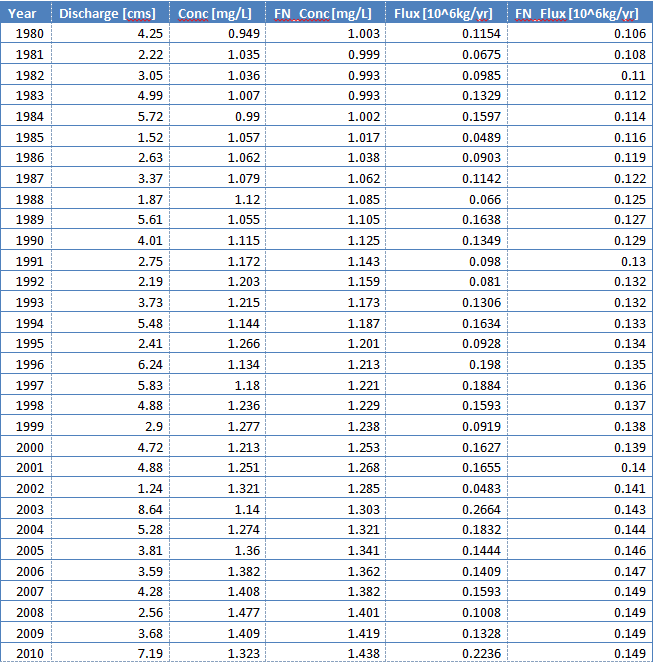
\includegraphics{table1.png}} 
\caption{A simple table produced in Microsoft Excel}
\label{overflow}
\end{figure}

%------------------------------------------------------------ 
\section{Saving Plots}
\label{app:savingPlots}
%------------------------------------------------------------
There are a variety of options for saving plots in R. Plots can be saved in JPG, PNG, PDF, and Postscript. JPG and PNG are easy to input into any number of programs (Microsoft Word or Powerpoint for example), but the images cannot be resized later. PDF and Postscript are easily re-sizable.

There are two steps to saving plots. The first is to declare the output type and file name by opening the 'device'. The second step is to turn off the device. Some simple examples should demonstrate this easily:

\begin{knitrout}
\definecolor{shadecolor}{rgb}{0.969, 0.969, 0.969}\color{fgcolor}\begin{kframe}
\begin{alltt}
\hlfunctioncall{jpeg}(\hlstring{"plotFlowSingle.jpg"})
\hlfunctioncall{plotFlowSingle}(1)
\hlfunctioncall{dev.off}()

\hlfunctioncall{png}(\hlstring{"plotFlowSingle.png"})
\hlfunctioncall{plotFlowSingle}(1)
\hlfunctioncall{dev.off}()

\hlfunctioncall{pdf}(\hlstring{"plotFlowSingle.pdf"})
\hlfunctioncall{plotFlowSingle}(1)
\hlfunctioncall{dev.off}()

\hlfunctioncall{postscript}(\hlstring{"plotFlowSingle.ps"})
\hlfunctioncall{plotFlowSingle}(1)
\hlfunctioncall{dev.off}()

\end{alltt}
\end{kframe}
\end{knitrout}


There are many additional options for each of these devices. See the R help files for more information. One option that would be useful for the larger fluxBiasEight graph is to adjust the height and width of the output. The output of fluxBiasEight is larger than the default pdf or postscript devices. Therefore, specifying the height and width eliminates R having to re-size the graphic:

\begin{knitrout}
\definecolor{shadecolor}{rgb}{0.969, 0.969, 0.969}\color{fgcolor}\begin{kframe}
\begin{alltt}
\hlfunctioncall{postscript}(\hlstring{"fluxBiasEight.ps"}, height=10,width=8)
\hlfunctioncall{fluxBiasEight}()
\hlfunctioncall{dev.off}()

\hlfunctioncall{pdf}(\hlstring{"fluxBiasEight.pdf"}, height=10,width=8)
\hlfunctioncall{fluxBiasEight}()
\hlfunctioncall{dev.off}()

\end{alltt}
\end{kframe}
\end{knitrout}




\clearpage
%------------------------------------------------------------
% BIBLIO
%------------------------------------------------------------
\begin{thebibliography}{10}

\bibitem{HirschI}
Helsel, D.R. and R. M. Hirsch, 2002. Statistical Methods in Water Resources Techniques of Water Resources Investigations, Book 4, chapter A3. U.S. Geological Survey. 522 pages. \url{http://pubs.usgs.gov/twri/twri4a3/}

\bibitem{HirschII}
Hirsch, R. M., Moyer, D. L. and Archfield, S. A. (2010), Weighted Regressions on Time, Discharge, and Season (WRTDS), with an Application to Chesapeake Bay River Inputs. JAWRA Journal of the American Water Resources Association, 46: 857-880. doi: 10.1111/j.1752-1688.2010.00482.x \url{http://onlinelibrary.wiley.com/doi/10.1111/j.1752-1688.2010.00482.x/full}

\bibitem{HirschIII}
Sprague, L. A., Hirsch, R. M., and Aulenbach, B. T. (2011), Nitrate in the Mississippi River and Its Tributaries, 1980 to 2008: Are We Making Progress? Environmental Science \& Technology, 45 (17): 7209-7216. doi: 10.1021/es201221s \url{http://pubs.acs.org/doi/abs/10.1021/es201221s}

\bibitem{HirschIV}
Moyer, D.L., Hirsch, R.M., and Hyer, K.E. (2012), Comparison of Two Regression-Based Approaches for Determining Nutrient and Sediment Fluxes and Trends in the Chesapeake Bay Watershed: U.S. Geological Survey Scientific Investigations Report: 2012-5244, 118 p. \url{http://pubs.usgs.gov/sir/2012/5244/}

\bibitem{HirschV}
Rice, K.C., and Hirsch, R.M. (2012), Spatial and temporal trends in runoff at long-term streamgages within and near the Chesapeake Bay Watershed: U.S. Geological Survey Scientific Investigations Report 2012–5151, 56 p. \url{http://pubs.usgs.gov/sir/2012/5151}


\end{thebibliography}

\end{document}

